\documentclass[11pt,twoside,a4paper,openright]{report}
\usepackage{a4wide}

\usepackage[DEM,newLogo]{uaThesis}
\def\ThesisYear{2018}

\usepackage[utf8]{inputenc}
\usepackage[english]{babel}
\usepackage{hyperref}
\usepackage{amsmath}
\usepackage{xspace}

\usepackage{arydshln}

\usepackage{csquotes}

\usepackage[citestyle=numeric]{biblatex}
\bibliography{bibliography.bib}

\usepackage[noabbrev, capitalize]{cleveref}
\usepackage{siunitx}
\sisetup{per-mode = symbol}
\usepackage{nicefrac}
\usepackage[official]{eurosym}

\usepackage{amsmath}
\usepackage{mathtools}

\usepackage{fancyvrb}
\usepackage{listings}

\usepackage{algpseudocode}
\usepackage{algorithmicx}
\usepackage{algorithm}

\usepackage{tikz}
\usetikzlibrary{positioning,shapes,shadows,arrows,backgrounds, patterns, shapes.multipart, calc}
\usepackage{tikz-3dplot}

\usepackage{graphicx}
\graphicspath{{images/}}

\usepackage{caption}
\usepackage{subcaption}

\usepackage{longtable}
\usepackage{rotating}
\usepackage[tableposition=top]{caption}
\usepackage{tabu}
\usepackage{booktabs}

% macros
\newcommand{\TF}[2]{\prescript{#2}{#1}{\mathcal{T}}}

\begin{document}


\TitlePage
\HEADER{\BAR}{\ThesisYear}

\TITLE{Bernardo Miguel \newline Martins Lourenço}
      {Reconstrução Tridimensional de Ambientes usando LIDAR e Câmara}
      
\vspace*{5mm}

\TITLE{}
      {Tridimensional Reconstruction of Scenes with LiDAR and Camera}

\smash{\rlap{\kern 80mm\lower 30mm\hbox{\Huge\textsf{\textbf{DOCUMENTO}}}}}%
\smash{\rlap{\kern 90mm\lower 42mm\hbox{\Huge\textsf{\textbf{PROVIS\'ORIO}}}}}%

\EndTitlePage
\titlepage\ \endtitlepage


\TitlePage
\HEADER{}{\ThesisYear}
\TITLE{Bernardo Miguel \newline Martins Lourenço}
      {Reconstrução Tridimensional de Ambientes usando LIDAR e Câmara}
      
\vspace*{5mm}

\TITLE{}
      {Tridimensional Reconstruction of Scenes with LiDAR and Camera}
\vspace*{15mm}

\TEXT{}
     {Dissertação apresentada à Universidade de Aveiro para cumprimento dos requisitos necessários à obtenção do grau de Mestre em Engenharia Mecânica, realizada sob a orientação científica de Miguel Armando Riem Oliveira, Professor Auxiliar do Departamento de Engenharia Mecânica da Universidade de Aveiro e de Paulo Miguel de Jesus Dias, Professor Auxiliar do Departamento de Eletrónica, Telecomunicações e Informática da Universidade de Aveiro.}
\EndTitlePage
\titlepage\ \endtitlepage


\TitlePage
\vspace*{55mm}
\TEXT{\textbf{o j\'uri~/~the jury\newline}}
     {}
\TEXT{presidente~/~president}
     {\textbf{Professor Doutor Vítor Manuel Ferreira dos Santos}\newline {\small
      Professor Associado com Agregação do Departamento de Engenharia Mecânica da Universidade de Aveiro}}
\vspace*{5mm}
\TEXT{vogais~/~examiners committee}
     {\textbf{Doutor Eurico Farinha Pedrosa}\newline {\small
      Bolseiro do Departamento de Eletrónica, Telecomunicações e Informática da Universidade de Aveiro (arguente)}}
\vspace*{5mm}
\TEXT{}
     {\textbf{Professor Doutor Miguel Armando Riem de Oliveira}\newline {\small
       Professor Auxiliar do Departamento de Engenharia Mecânica da Universidade de Aveiro (orientador)}}

\EndTitlePage
\titlepage\ \endtitlepage % empty page


\TitlePage
\vspace*{55mm}
\TEXT{\textbf{agradecimentos~/\newline acknowledgements}}
     {}
\EndTitlePage
\titlepage\ \endtitlepage


\TitlePage
\vspace*{55mm}
\TEXT{\textbf{Resumo}}
     {Resumo pt}
\EndTitlePage
\titlepage\ \endtitlepage % empty page

\TitlePage
\vspace*{55mm}
\TEXT{\textbf{Abstract}}
     {Resumo EN}
\EndTitlePage
\titlepage\ \endtitlepage % empty page


\pagenumbering{roman}

\tableofcontents
\cleardoublepage
\listoffigures
\cleardoublepage
\listoftables

\cleardoublepage

\pagenumbering{arabic}
\chapter{Introduction}

Digital reconstruction of three dimensional scenes is a field that gained a high importance in areas like architecture, robotics, archeology and autonomous driving. As an example, virtual reality technologies allows high-detail and high-resolution models to be experiences in an immersive 3D experience, and the technology is becoming available for the general public, as prices for this 3D headsets and VR-ready phones decrease. These new technologies create a demand for reconstruction technology and new algorithms that are accurate and of high quality.

\section{Motivation}

Despite all the work done, there is still no perfect solution. 3D reconstruction is still a challenge, because real scenes are very complex and measurements are subject to errors and noise. Past experience tells that a single sensor is not enough to model real environments, so currently the process lies into using multiple sensors and trying to merge the data from all the sensors, in order to capture a more realistic model.

However, this introduces a set of other problems inherent to this approach. For example, the data from different sensors needs to be merged accurately. Also, the positions of all the sensors need to be known accurately, which means that the calibration processes need to be more robust and precise.

Also, current reconstruction algorithms require a large amount of manual work, which means that a reconstruction require many man-hours to be completed, which is unfeasible for most applications. One of the goals of reconstruction is to develop algorithms that are automatic and do not require any intervention, making it faster and more accessible. 

An automatized reconstruction method is still a challenge today, but new algorithms could allow it, which would make reconstruction work more accessible.

Nowadays, 3D reconstruction software is even available in smartphones, usually targeting Augmented Reality applications. However, these 3D reconstructions are not accurate and the resulting models are far from perfect.

\section{Problem Description}

Nowadays, Lidar laser scanners are becoming more available and more accessible,  and because of their properties, as their high precision and high range, became an unmatched technology for 3D reconstruction. The lidar lasers are available as 2D laser scanners or 3D laser scanners, like the Velodyne. Despite their immense potential, 3D laser scanner is still a very expensive solution and cheaper solutions are comprised of a cheaper 2D laser scanner mounted on a moving frame. This solution, despite its low cost, can achieve good results, but requires a fine calibration. 

Also, laser scanners do not register the color information, so a common practice is to pair the laser scanner with a camera to get both geometric and color data. This method also requires a fine calibration between both sensors to correctly merge the data. 

\section{Objectives}

The objective is to develop a fully integrated solution for 3D acquisition using both laser and image data. This objective was divided into four main objectives.

The first objective was to develop a 3D laser scanner, consisting of a laser scanner and a camera, and capable of recording data from both sensors in a fast and semi-autonomous way.

The second objective was to define a methodology to record the data from the scene. This methodology should take into account the limitations of both sensors and try to minimize their effect in the final result.

The third objective was to develop a set of methods to reconstruct the geometry of the scene reliably. The main challenge is the extrinsic calibration of the laser, because it is fundamental for a reliable reconstruction. So, a new calibration method was developed to achieve the wanted results.

The fourth and final objective was to develop a set of methods to merge the image data with the geometry of the scene, to reconstruct the color.

The final result is then, a point cloud with color and geometric information.

\section{Document Outline}

This dissertation is composed of eight chapters, which are arranged as follows:

\begin{description}
    \item[Introduction] The current chapter, in which the description of the problem is shown and the objectives of this work are defined.
    \item[State of Art] Describes the technologies and solutions found in the field of 3D reconstruction, both commercial and academic, as well of a small technical background on this solutions.
    \item[Experimental Infraestructure] Introduces all the software and hardware used to develop this work. In particular, the mobile robot for 3D scanner is described.
    \item[Methodology for Scene Capture] Describes the methods and algorithms used to reconstruct the geometry of the scene, using the laser scan data recorded.
    \item[Methodology for Image Reconstruction] Describes the methods and algorithms used to reconstruct the color information of the scene, using the camera images recorded.
    \item[Result and Discussion] Presents and discusses the experimental results obtained in this work.
    \item[Conclusion and Future Work] Summarizes the overall work developed and present possible future work.
\end{description}
\chapter{State of Art}

\section{Technologies}

Many technologies were developed to capture tridimensional information of the environment. The following section describes such systems and describe the basic working principle along with the pros and cons inherent to each ones. These techniques can be categorized into triangulation and time-of-flight.

\subsection{Stereoscopy}

For many years, stereoscopy remained the most popular method for 3D sensing, also because its working principle resembles the human stereoscopic vision. This system uses images taken from a pair of cameras and extracts depth information using the perspective projection: the position of objects closer differ more than objects farther. To compute depth, features from both images are extracted and matched together, which makes it a complex and computationally demanding, so it requires fast computers or dedicated software. This system has the advantage of having a good rate of acquisition and having high resolution. Also, color information is available. However, the reconstruction algorithm rely heavy on environment characteristics, like lightning conditions, texture and non-homogeneous regions~\cite{klimentjew2010}. This means that this method gives good results for edges and textured areas, but fails to get the depth information of continuous surfaces. Also, the poor geometric precision is one of the limitation of this system.

\subsection{Structured Light}

In 2010, the availability of consumer grade depth sensors based on structured light lead to the development of consumer-grade small factor RGB-D cameras, started by Microsoft, with the \textit{Kinect} and followed by other devices, like \textit{ASUS Xtion} and \textit{Intel RealSense}. These cameras come in small form factors, are inexpensive and are capable of capturing both color and depth information at real-time rates~\cite{zollhoefer2018}.

These appealing characteristics lead to a huge research and development in 3D reconstruction using this camera, culminating in the KinectFusion algorithm \cite{kinectfusion2011}, capable of a fast and precise 3D reconstruction using a \textit{Kinect} RGB-D camera and commodity GPUs. This algorithm was capable of performing real-time reconstruction, using a Iterative Closest Point (ICP) for tracking the location of the device and for the registration of new RGB-D data. Nowadays, it is possible to achieve the same result using a phone equipped with a depth camera, like the \textit{Lenovo Phab 2} or \textit{ASUS Zenphone VR} and with the \textit{Google Tango} software. 

Structured light sensors work by projecting an infrared pattern onto the scene and calculate the depth via the perspective deformation of the pattern due to the different object's depth. However, this technique yields sub-optimal results: the depth values from structured light have significant error or can be missing, specially from objects with darker colors, specular surfaces or small surfaces~\cite{shen2013}. 

\subsection{Time of Flight}

Time of flight sensors, or ToF sensors, use the speed of light to measure the distance. A scene is illuminated by a light source and the reflected light is detected back by the sensor. The time that the light has taken to travel forth and back is then measured and the depth is calculated with this time. The measurement dependes on the type of ToF system used, that is ether \textit{continuous} or \textit{pulsed}. In \textit{pulsed} systems, light is emitted in bursts with a fast shutter and the time between the emission and the reception is calculated. \textit{Continuous} systems use a modulated light source and measure the phase-shift between the outgoing and incoming wave.

This technology has some advantages comparing to both previous approaches \cite{zollhoefer2018}. First, it is less computationally intensive, because the measurement is directly done by a specialized sensor. Second, it is partially independent of the lightning conditions because the light detected is emitted by the device itself. Further, it is capable of providing a dense and accurate depth values, even for continuous or irregular surfaces, unlike the stereoscopic approach. Moreover, it is much faster that any other method, capable of acquisition rates of hundreds of \si{\hertz}. However, it has some disadvantages as well. Unlike stereoscopic, which is a passive method, ToF sensors interact with the scene, so are not possible to be implemented in certain environments. Also, the properties of the material, like the reflectivity, color and roughness can have significant effects on the accuracy of ToF sensors. Moreover, multi-path reflections are a common problem of ToF sensors, caused by multiple reflections of the light, causing errors in the measurements. Furthermore, interference can exist if multiple ToF sensors share the same environment. However, it is possible to mitigate this effect, by either controlling the sensor such that only one is activate at a time, or by using different modulation frequencies in their illumination source.

A popular ToF sensor nowadays is the Photonic-Mixer-Device camera, which looks similarly to a normal image sensor, but measures the phase shift of incoming light. This sensor is now being used in new generation RGB-D cameras, replacing the structured light approach, mainly because it is more resilient to background light, allowing the sensor to work in outdoor environments \cite{zollhoefer2018}. One of this example is the new \textit{Kinetic 2}, that replaced the last depth sensor with this one.

\subsection{LiDAR}

Light Detection and Ranging, or LiDAR, is one of the most precise and reliable ways to measure distances. It began being used shortly after the invention of Laser, in 1960, and it's valuable characteristics lead to the integration of it in the Apollo 15 mission, to serve as an altimeter to map the surface of the moon. Soon after, it was implemented in aircrafts to create high-precision and dense earth's surface models. Nowadays, its applications can be found everywhere where an accurate distance measurement is required, as for example in geology, archeology, geography and meteorology.

The success of LiDAR is related to the use of laser as its light source. Lasers are capable of emitting beams of light that are monochromatic, narrow and polarized. That is, lasers emit light in a narrow spectrum, so they can produce a single color of light, also known as monochromatic light. It improves the resilience against background light, making it possible to use even with sun light. Also, laser photons travel parallel, creating a narrow beam that stays narrow even at large distances, with minimum scattering, therefore measuring the distance in a very small area in the surface. This improves the measurements near sharp transitions, where a bigger area of measurement can cause errors in the measurement. Moreover, lasers can transition between an on-off state in a very short time. This is significant to reduce the error of the distance measurement, because it is directly influenced by the time between pulses, and a sharp transition reduces the error in the time measurement. 

The first major application of LiDAR technology was to map and reconstruct the topology of the earth's surface. To do it, high range laser scanners are mounted on a plane and are flown above the target area. This is possible due to their high power laser, which allows ranges in the kilometer range, while maintaining precision in the centimeter range. This lasers also have a high sampling rate, in the order of the kilohertz, which is essencial to maintain a dense sampling, even at high travelling speeds. This high sampling also allows the terrain to be mapped even with high vegetation, because even that only a small percentage of points reach the terrain, there are still a significant number of points. This is just not possible with other methods, like aerial photography. 

Moreover, airborne LiDAR is also used to detect and classify clouds, which is an important data in meteorology. This is possible by studying the rayleigh scattering effect, which occurs when a laser beam goes through a particles smaller that its wave length, as for example, the water molecules in clouds.  This is essential for modern forecast prediction.

A airborne LiDAR scanner of the Austrian city Retz is shown in \cref{fig:riegl-lidar-scan}, which is available in \cite{potree-retz}, taken with a Riegl laser scanner placed in a Unmanned Aerial Vehicle. \cref{fig:riegl-lidar-scan-big} shows the entire scan with an area of \SI{1300 x 1300}{\meter}, \cref{fig:riegl-lidar-scan-small} shows a portion correspondent to the city, and \cref{fig:riegl-lidar-scan-tiny} shows the town hall, which has an area of about \SI{150 x 70}{\meter}. As can be seen, the result is a massive point cloud that covers a large area while still maintaining a high point density so small details are not smeared out. 

\begin{figure}[p]
    \centering
    \begin{subfigure}{\textwidth}
        \centering
        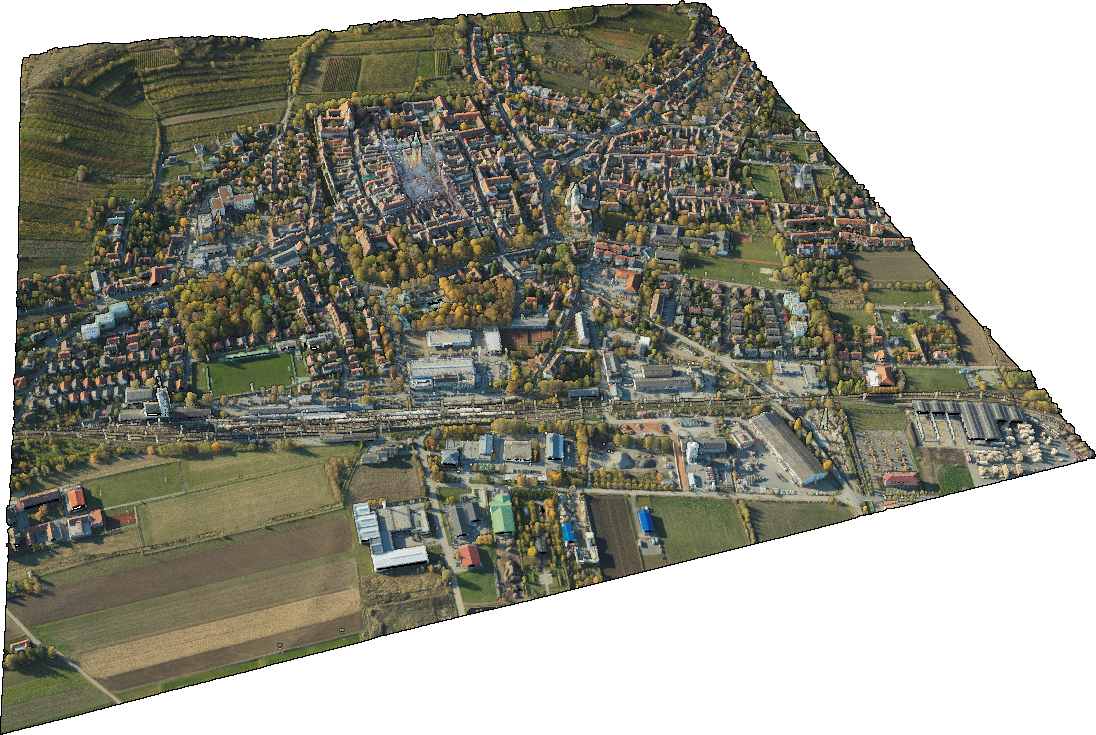
\includegraphics[width=.65\textwidth]{riegel-lidar-scan-big}
        \caption{The entire scan.}
        \label{fig:riegl-lidar-scan-big}
    \end{subfigure}

    \centering
    \begin{subfigure}{\textwidth}
        \centering
        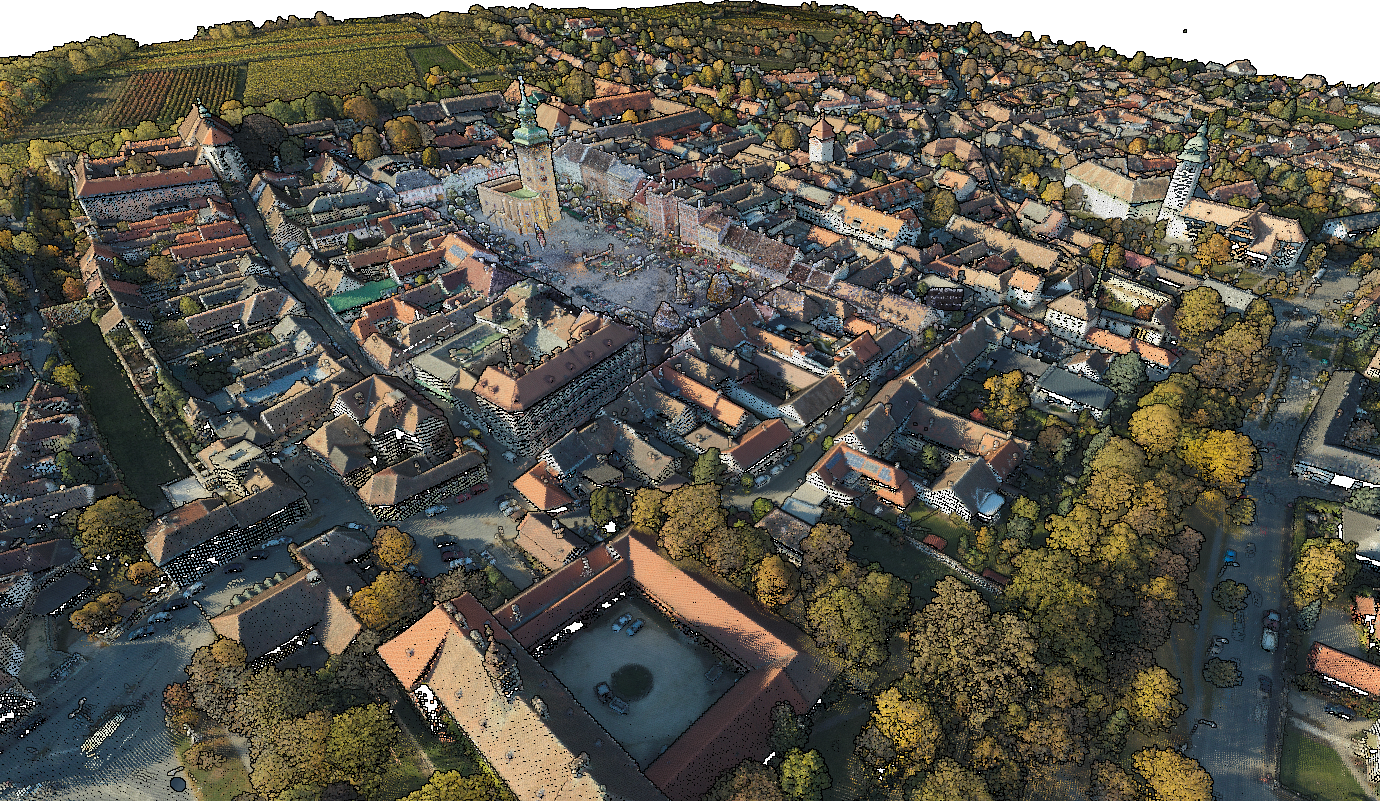
\includegraphics[width=.65\textwidth]{riegel-lidar-scan-small}
        \caption{Pormenor of the City.}
        \label{fig:riegl-lidar-scan-small}
    \end{subfigure}

    \centering
    \begin{subfigure}{\textwidth}
        \centering
        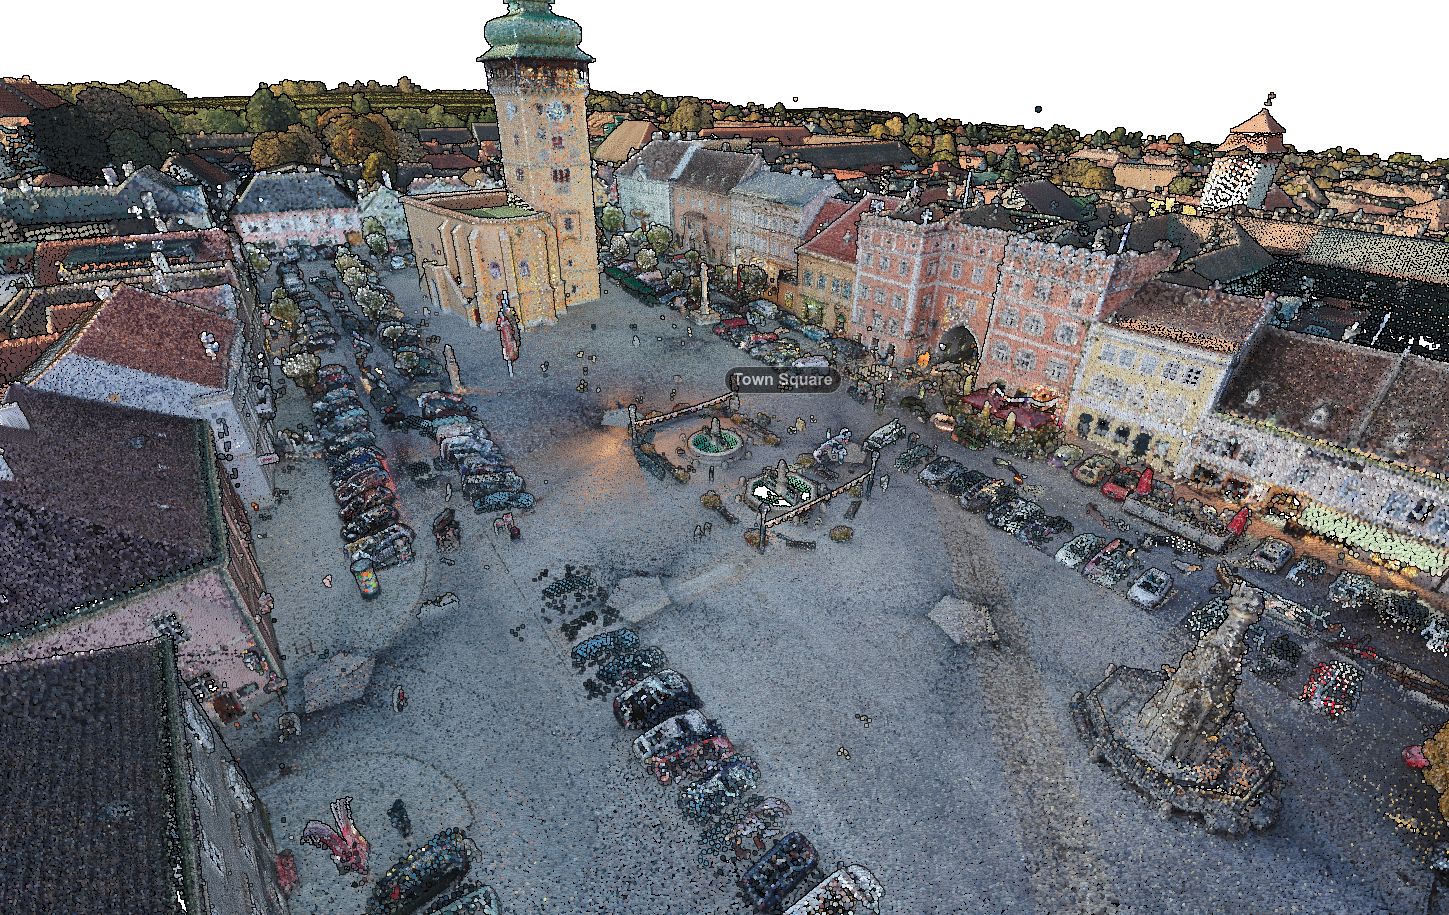
\includegraphics[width=.65\textwidth]{riegel-lidar-scan-tiny}
        \caption{Pormenor of the Town Hall.}
        \label{fig:riegl-lidar-scan-tiny}
    \end{subfigure}

    \caption{Point cloud of Retz obtained by an airborne LiDAR.}
    \label{fig:riegl-lidar-scan}
\end{figure}

In recent years, LiDAR scanner became a fundamental technology for industrial and robotics applications. Their small form factor and high precision are essencial for numerous applications. In general, two types of laser scanners exist: the 2D laser scanners and the 3D laser scanners. 

2D laser scanners emit a single laser beam, which is reflected by a rotating mirror to scan across a planar area, as seen on figure X. They are also the most accessible type, as their price ranges range from hundreds to tenths of thousands of Euros, depending on their characteristics. One example of this laser scanners is the SICK LMS511, shown in \cref{fig:sick-lms511}. 

\begin{figure}
    \centering
    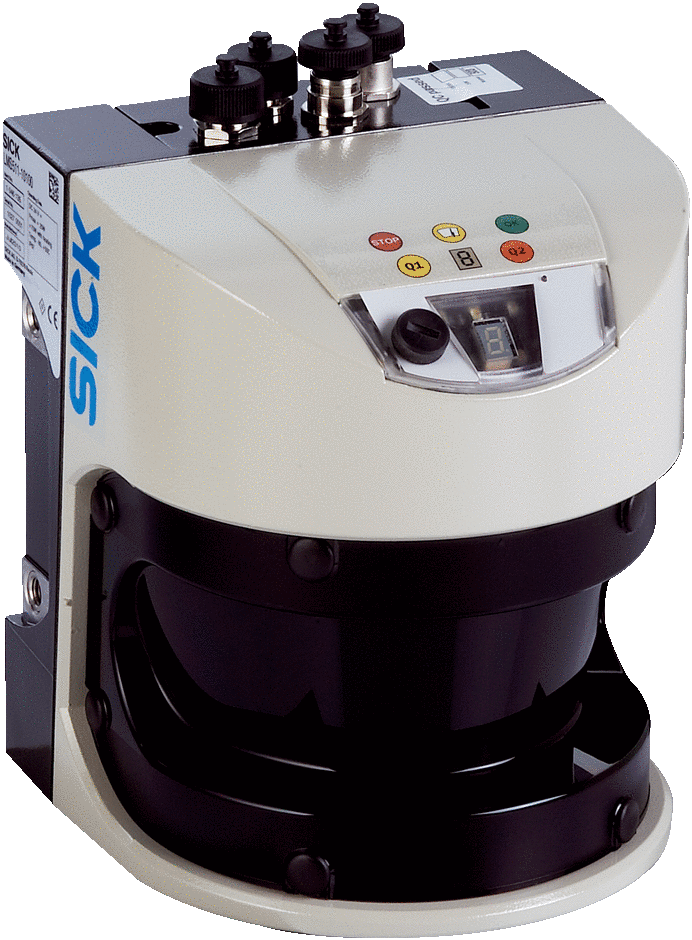
\includegraphics[width=6cm]{lms511}
    \caption{Sick LMS511 2D laser scanner.}
    \label{fig:sick-lms511}
\end{figure}

This laser scanners have a large number of applications. For example, 2D laser scanners are used in autonomous robots, to provide precise 2D mapping information of the environment, which can be user afterwards for location and navigation \cite{siritanawan17}. Compared to other technologies, like stereo vision, this one requires small processing power and yields accurate results, so their application is easy to implement and requires low processing power. 

Another widely used application is intrusion detection. The 2D laser scanner can be spaced in a room or door to detect if any object enters to the space. For example, it is used to ensure the safety of workers in industrial environment, ensuring that workers do not get close to working machines. Other example is in theft prevention in museums and banks to secure specific areas against robbery or vandalism \cite{sick-security}.

Recently, 3D laser scanners become available, but at a high price range. One example of these new sensors is the Velodyne, which is a 3D laser scanner capable of producing a 3D point cloud directly, unlike the 2D laser scanner. This is possible because they emit multiple laser beams, instead of just one. The laser beams are reflected using a rotating mirror, to get a continuous 3D scan. Moreover, 3D laser scanners are capable of producing a 3D scan at a higher rate than any solution employing a 2D laser scanner. In the case of Velodyne \emph{VLS-128}, shown in \cref{fig:velodyne-vls128}, the number of simultaneous laser beams are \num{128}, with a vertical Field of View of \SIrange{-25}{+15}{\degree} and up to \SI{300}{\meter} range\cite{velodyne-vls128}. This LiDAR laser is capable of a sampling rate of about 9.6 million points per second.

\begin{figure}[h]
    \centering
    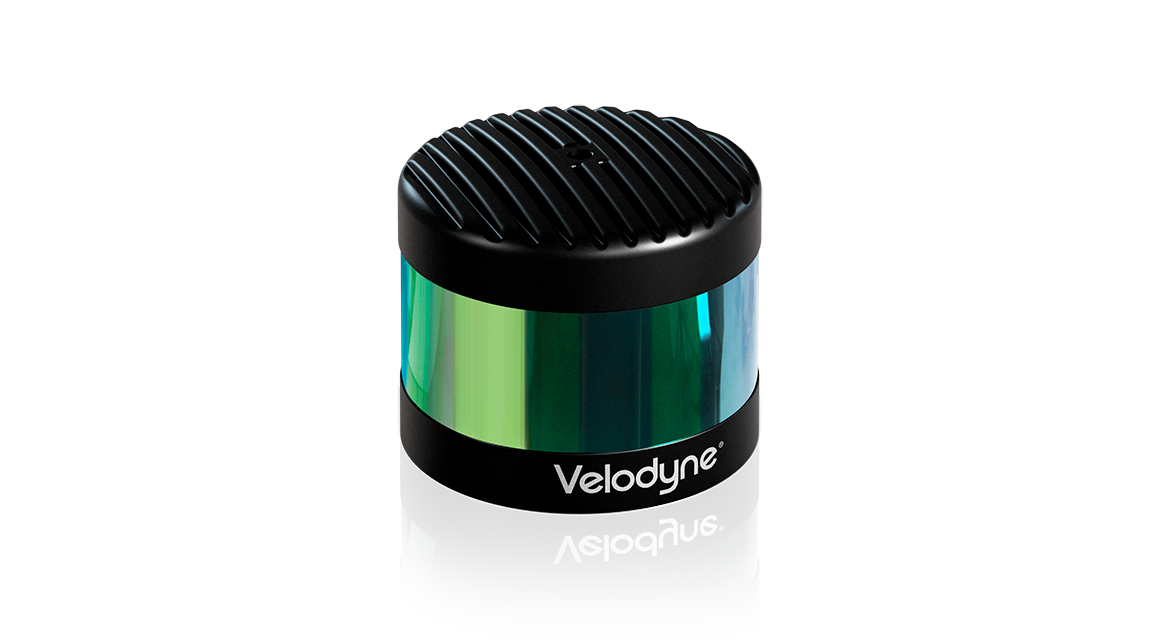
\includegraphics[width=8cm]{velodyne-vls128}
    \caption{Velodyne VLS128 LiDAR laser scanner.}
    \label{fig:velodyne-vls128}
\end{figure}

3D laser scanners are a very new technology, and are mostly used for high research projects, mainly in autonomous vehicles, like the Google Autonomous car \cite{google-self-driving} or the Stanford Junior Vehicle\cite{montemerlo08}. This application benefits mostly from this scanners high sampling ranges and \SI{360}{\degree} horizontal field of view.

\begin{figure}[h]
    \centering
    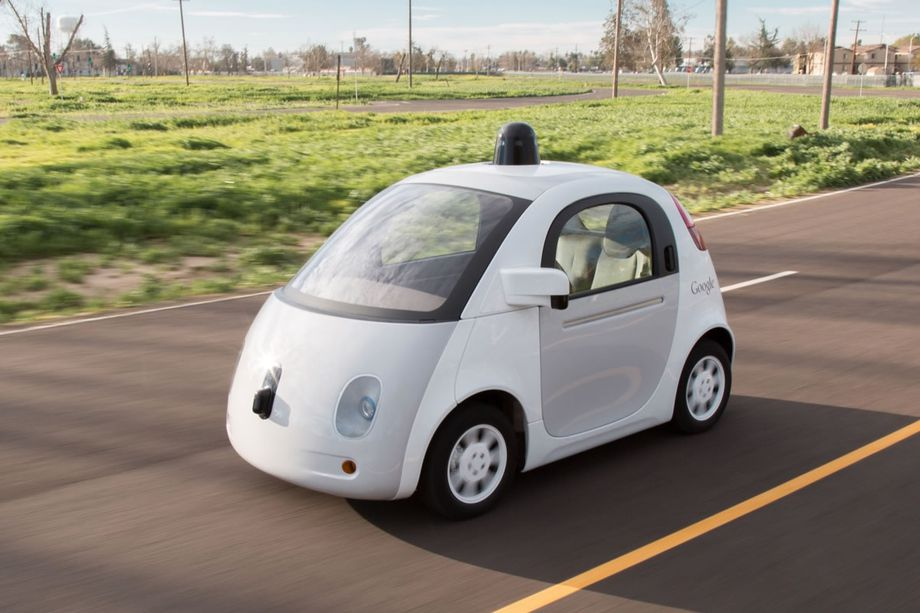
\includegraphics[width=8cm]{google-autonomous-car}
    \caption{Google Autonomous Car.}
    \label{fig:google-autonomous-car}
\end{figure}

\section{Related Academic Work}

Many scientific studies can already be found concerning the research and development of 3D sensors using laser scanners. In most studies, a cheaper alternative using 2D laser scanners is build instead of a more expensive 3D solution. In order to create a full 3D scan, the 2D laser is mounted on top of a moving platform and each individual laser scan is registered on a static frame of reference. The motion of the laser scanner can be classified as continuous or discontinuous. Usually a continuous motion is used for real-time systems, like autonomous vehicles, while a discontinuous motion is used when real-time is not important, like accurate 3D reconstructions of scenes. In the following paragraphs such systems that were developed so far are described.

In \cite{surmann2003}, a mobile robot was capable of autonomous navigation, thanks to a tilting \textit{LMS200} laser scanner, that provided a depth map of the front of the robot, with a maximum resolution of $721\times256$ points. However, a scan of $181\times256$ points took about \SI{3.4}{\second}, and scans with more points ($361$ or $721$) meant double or quadruple this time, making it not suitable for real-time operation. This previous system had a limited field of view, so in \cite{zcai05} a \textit{LMS291} was mounted on a pan-tilt unit for generating a 3D point cloud with a parameterized field of view.

More recently, 3D laser scanner began being developed for continuous operation for real-time for Simultaneous Mapping and Navigation, or SLAM, for autonomous robots. This was specially due to the \textit{DARPA Grand Challenge}, a competition to award the fastest autonomous unmanned vehicle that completed a 300 miles track. In \cite{maurelli2009}, a 3D laser scanner (\cref{fig:maurelli-laser-scanner}) was developed by placing two \textit{LMS200} planar laser scanners on a rotating vertical axis, capable of generating a high-quality 3D point cloud with a \SI{360}{\degree} field of view. Lots of other lasers were developed by rotating the laser in a continuous motion using a turntable \cite{nemoto2007}, a swinging platform \cite{yoshida11}. This sensor also became lighter, compact and modular, making it possible to integrate in multiple systems easily. One of this systems is \textit{KaRoLa} (\cref{fig:karola}), described in \cite{karola14}. This laser scanner was then applied to several system, specially in search and rescue robots.

\begin{figure}[h]
    \centering
    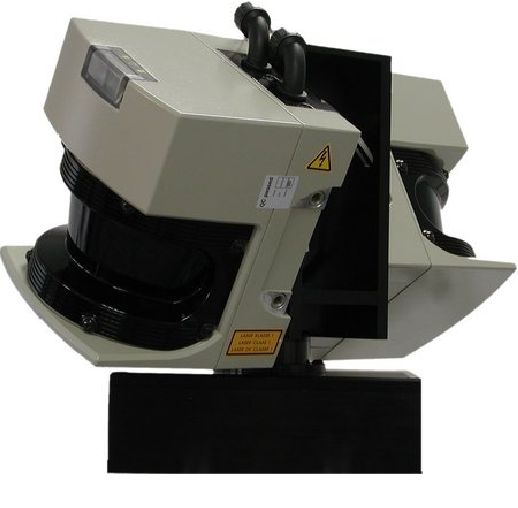
\includegraphics[width=5cm]{maurelli-laser}
    \caption{3D laser scanner developed in \cite{maurelli2009}.}
    \label{fig:maurelli-laser-scanner}
\end{figure}

\begin{figure}[h]
    \centering
    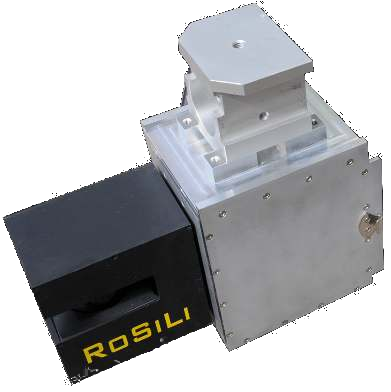
\includegraphics[width=5cm]{karola}
    \caption{The KaRoLa 3D laser scanner.}
    \label{fig:karola}
\end{figure}

The 3D laser sensors are only able to reconstruct the geometry of the scene. Some sensors are also able to measure the intensity of the reflected light, create a grayscale value for each point. This intensity is measured, of course, in the frequency spectrum of the emitted light of the sensor, which is usually infrared (\SI{950}{\nano\meter}). To reconstruct the color, one or more cameras are coupled to the sensor, and both depth and color data is merged, in a process called fusion, to create colorized model. This is specially important for areas like architecture or archeology, where color information is very important. Such work can be seen on \cite{pdias2006}, where a 3D sensor like the one described in \cite{surmann2003} was paired with a camera, to generate a 3D reconstruction with color. Another technique was created in \cite{stamus2000}, where the range and color images are captured separately and then a method is used to make the registration of the color images in respect to the extracted geometry. The registration was optimized for scenes with high geometry content.

These techniques are applied, for example, in cultural heritage, to model important art pieces. One of the most famous examples is the Michelangelo project \cite{levoy2000}, which developed a technique to register data from a triangulation sensor and color image data to reconstruct the 3D geometry of the statue of Michelangelo's David. One of the challenges in this project was to capture the chisel marks in the surface of the status, requiring a resolution of \nicefrac{1}{4} \si{\milli\meter}, in a statue \SI{5}{\meter} tall~\cite{levoy2000}.

\section{Comercial Solutions}

In this section two commercial solutions are shown and discussed. Both solution aim for a precise 3D reconstruction with color information, but the first solution does it with a structured light sensor and the second solution relies on a laser scanner. 

\subsection{Matterport}

\emph{Matterport} is advertized as an all-in-one solution, capable of both 3D reconstruction and capture 4K resolution images from the scene. Their target is mostly the reconstruction of indoor scenes, more specifically, the interior of houses. Then, the 3D model can be used to showcase the interior of the house, using both virtual reality or panoramic photography, or to make 3D measurements and automatically generate floor plans\cite{matterport}.

\emph{Matterport} offers two products: a 3D camera and a cloud service to process the raw data taken with the camera. The camera, as seen in \cref{fig:matterport-camera}, consists of two sensors: a structured light sensor and a photographic camera\cite{matterport}. The structured light sensor has an advertized $99\%$ geometric accuracy within the \SI{4.5}{\meter} maximum range. The Photography sensor is a 4K HDR camera.

\begin{figure}[h]
    
    \centering
    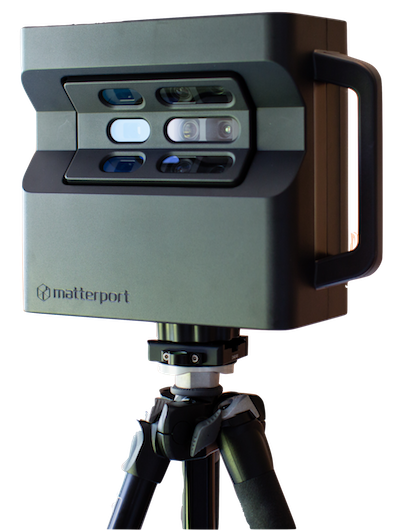
\includegraphics[width=5cm]{matterport}

    \caption{Matterport Pro2 Camera.}
    \label{fig:matterport-camera}

\end{figure}

The overall process to capture a scene is fast and easy: the 3D camera is placed on a tripod and is controlled remotely. Each acquisition takes about \SI{20}{\second} and the result is a 3D colorized mesh with 4 million vertices and a \SI{360}{\degree} panoramic photography with 134.2 MP. To scan an entire environment, an operator moves the camera to each space and make multiple new acquisitions from that space.

A set of models reconstructed from the with the Matterport solution can be found in \cite{matterport-gallery}. As an example, the model named "Pennsylvania Craftsman Home" \cite{matterport-house} can be seen in \cref{fig:matterport-model}. This model represents the complete interior of an house and looks very realistic.

\begin{figure}[h]
    
    \centering
    \begin{subfigure}{\textwidth}
        \centering
        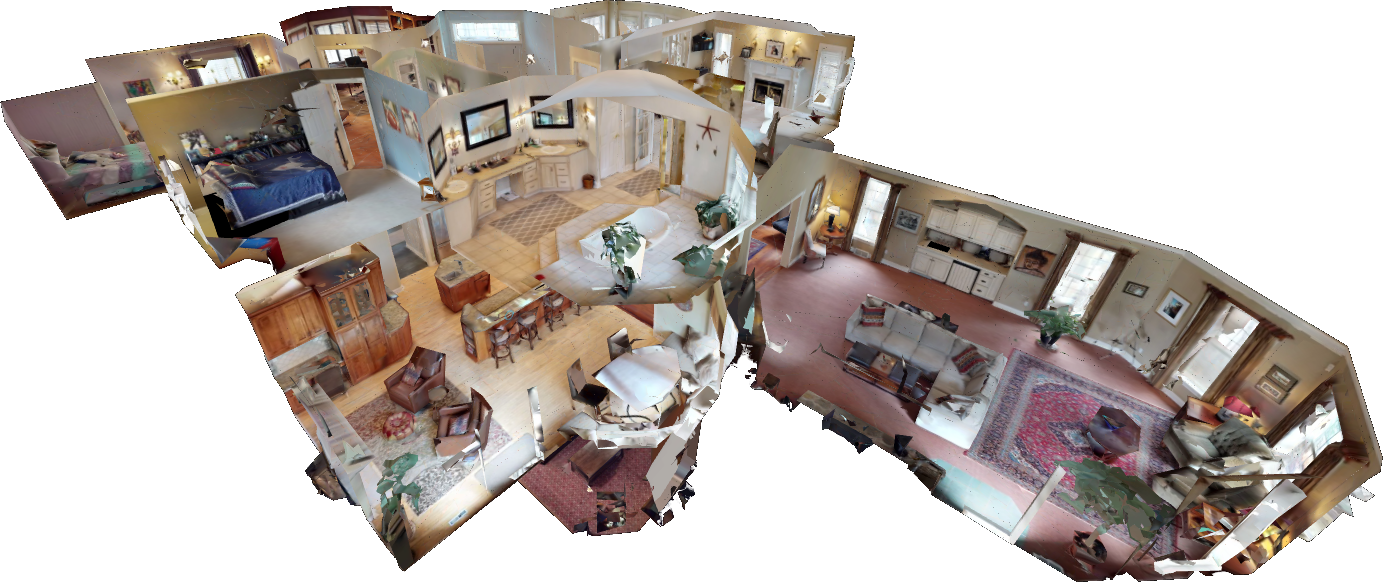
\includegraphics[width=10cm]{matterport-scan-side}
        \caption{Side view.}
    \end{subfigure}

    \begin{subfigure}{\textwidth}
        \centering
        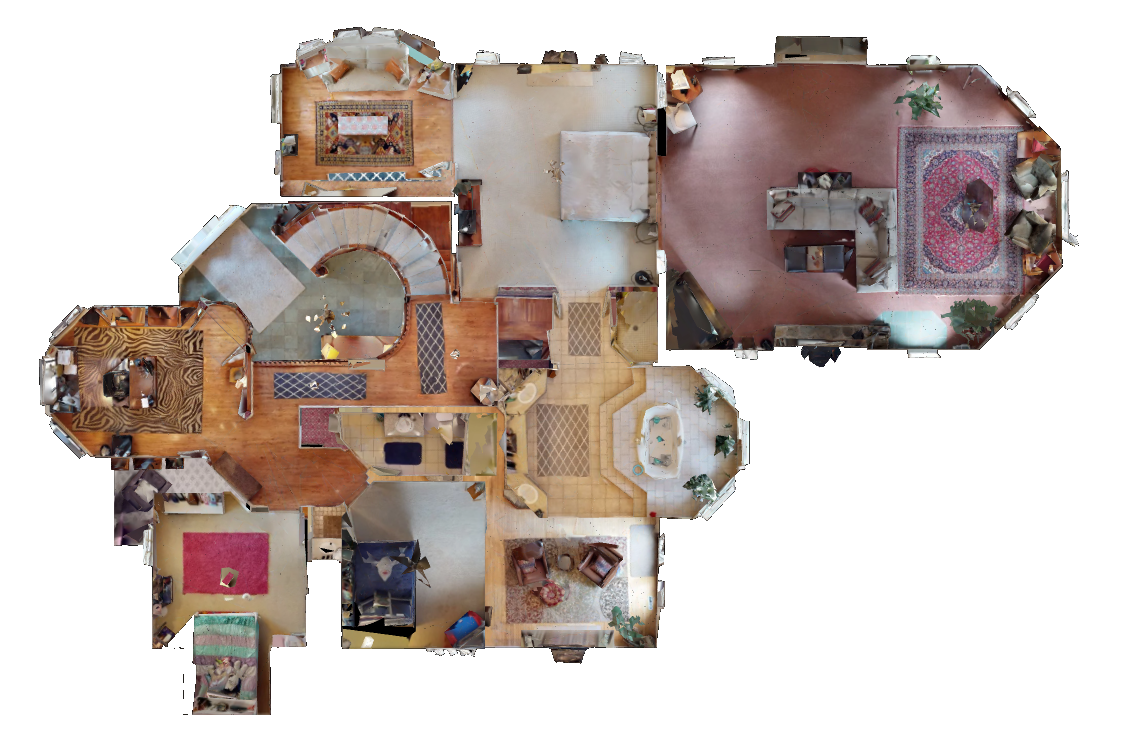
\includegraphics[width=10cm]{matterport-scan-top}
        \caption{Top view.}
    \end{subfigure}

    \caption{Matterport "Pennsylvania Craftsman Home" model (from~\cite{faro-scan}).}
    \label{fig:matterport-model}
\end{figure}

\subsection{Faro Focus}

Faro Focus \cite{faro-focus} are a series of 3D laser scanners targeted for the sectors of architecture, engineering, construction and product design. As such, this solution is capable of fast 3D reconstructions both on outside and inside environments with great accuracy. The 3D scanner, as seen in \cref{fig:faro-focus}, is design for portability and is equipped with a laser scanner with a precision of \SI{+-1}{\milli\meter} and a range of \SIrange{0.6}{350}{\meter}, and a 8 MP HDR camera.

\begin{figure}[h]
    \centering
    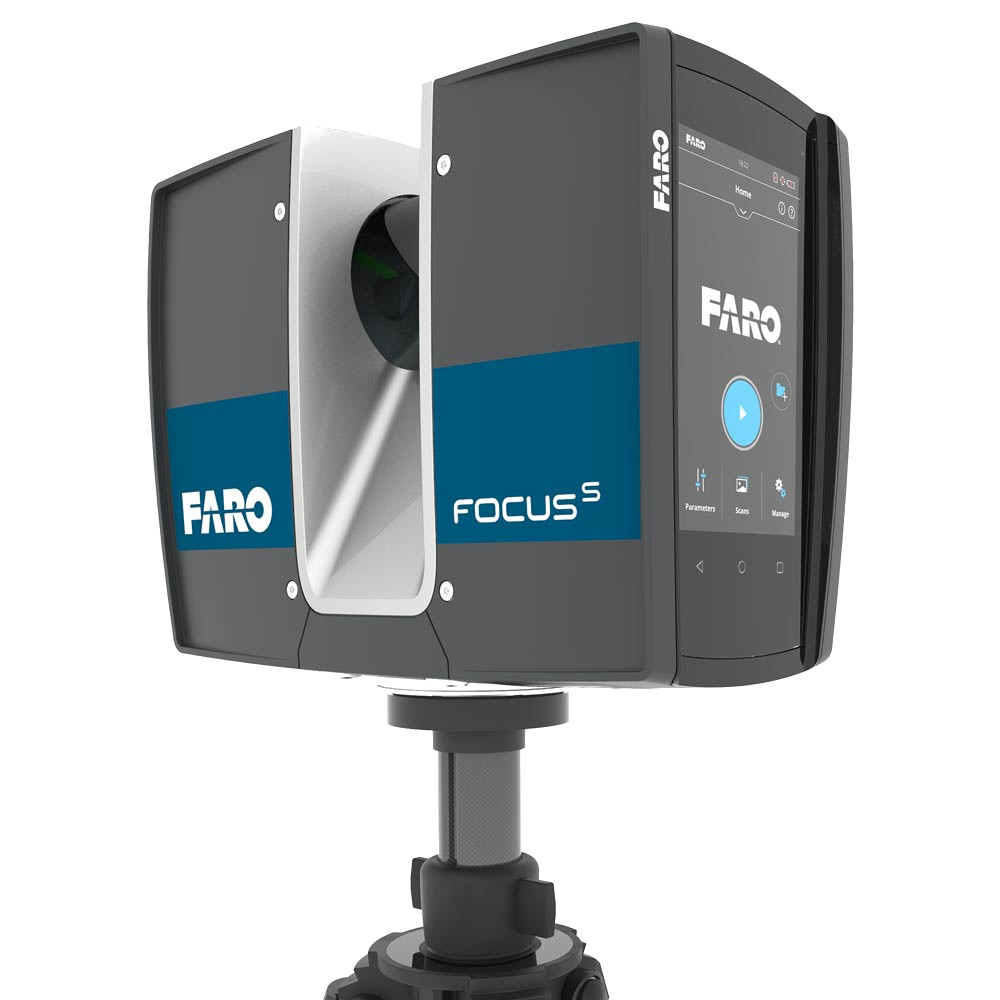
\includegraphics[width=6cm]{faro-focus}
    \caption{Faro Focus 3D laser scanner.}
    \label{fig:faro-focus}
\end{figure}

An acquisition, like in the \emph{Matterport Pro2 Camera}, is quick and easy, but does not require any remote computer, as the scanner incorporates a touch LCD screen. All the subsequent processing is done afterwards in a computer, using their proprietary software.

Faro Focus scans are very precise, as they are used for precise measurements of the reconstructed scene. As an example, a scan obtained by the Faro Focus can be seen in \cref{fig:faro-scan}.

\begin{figure}[h]
    \centering
    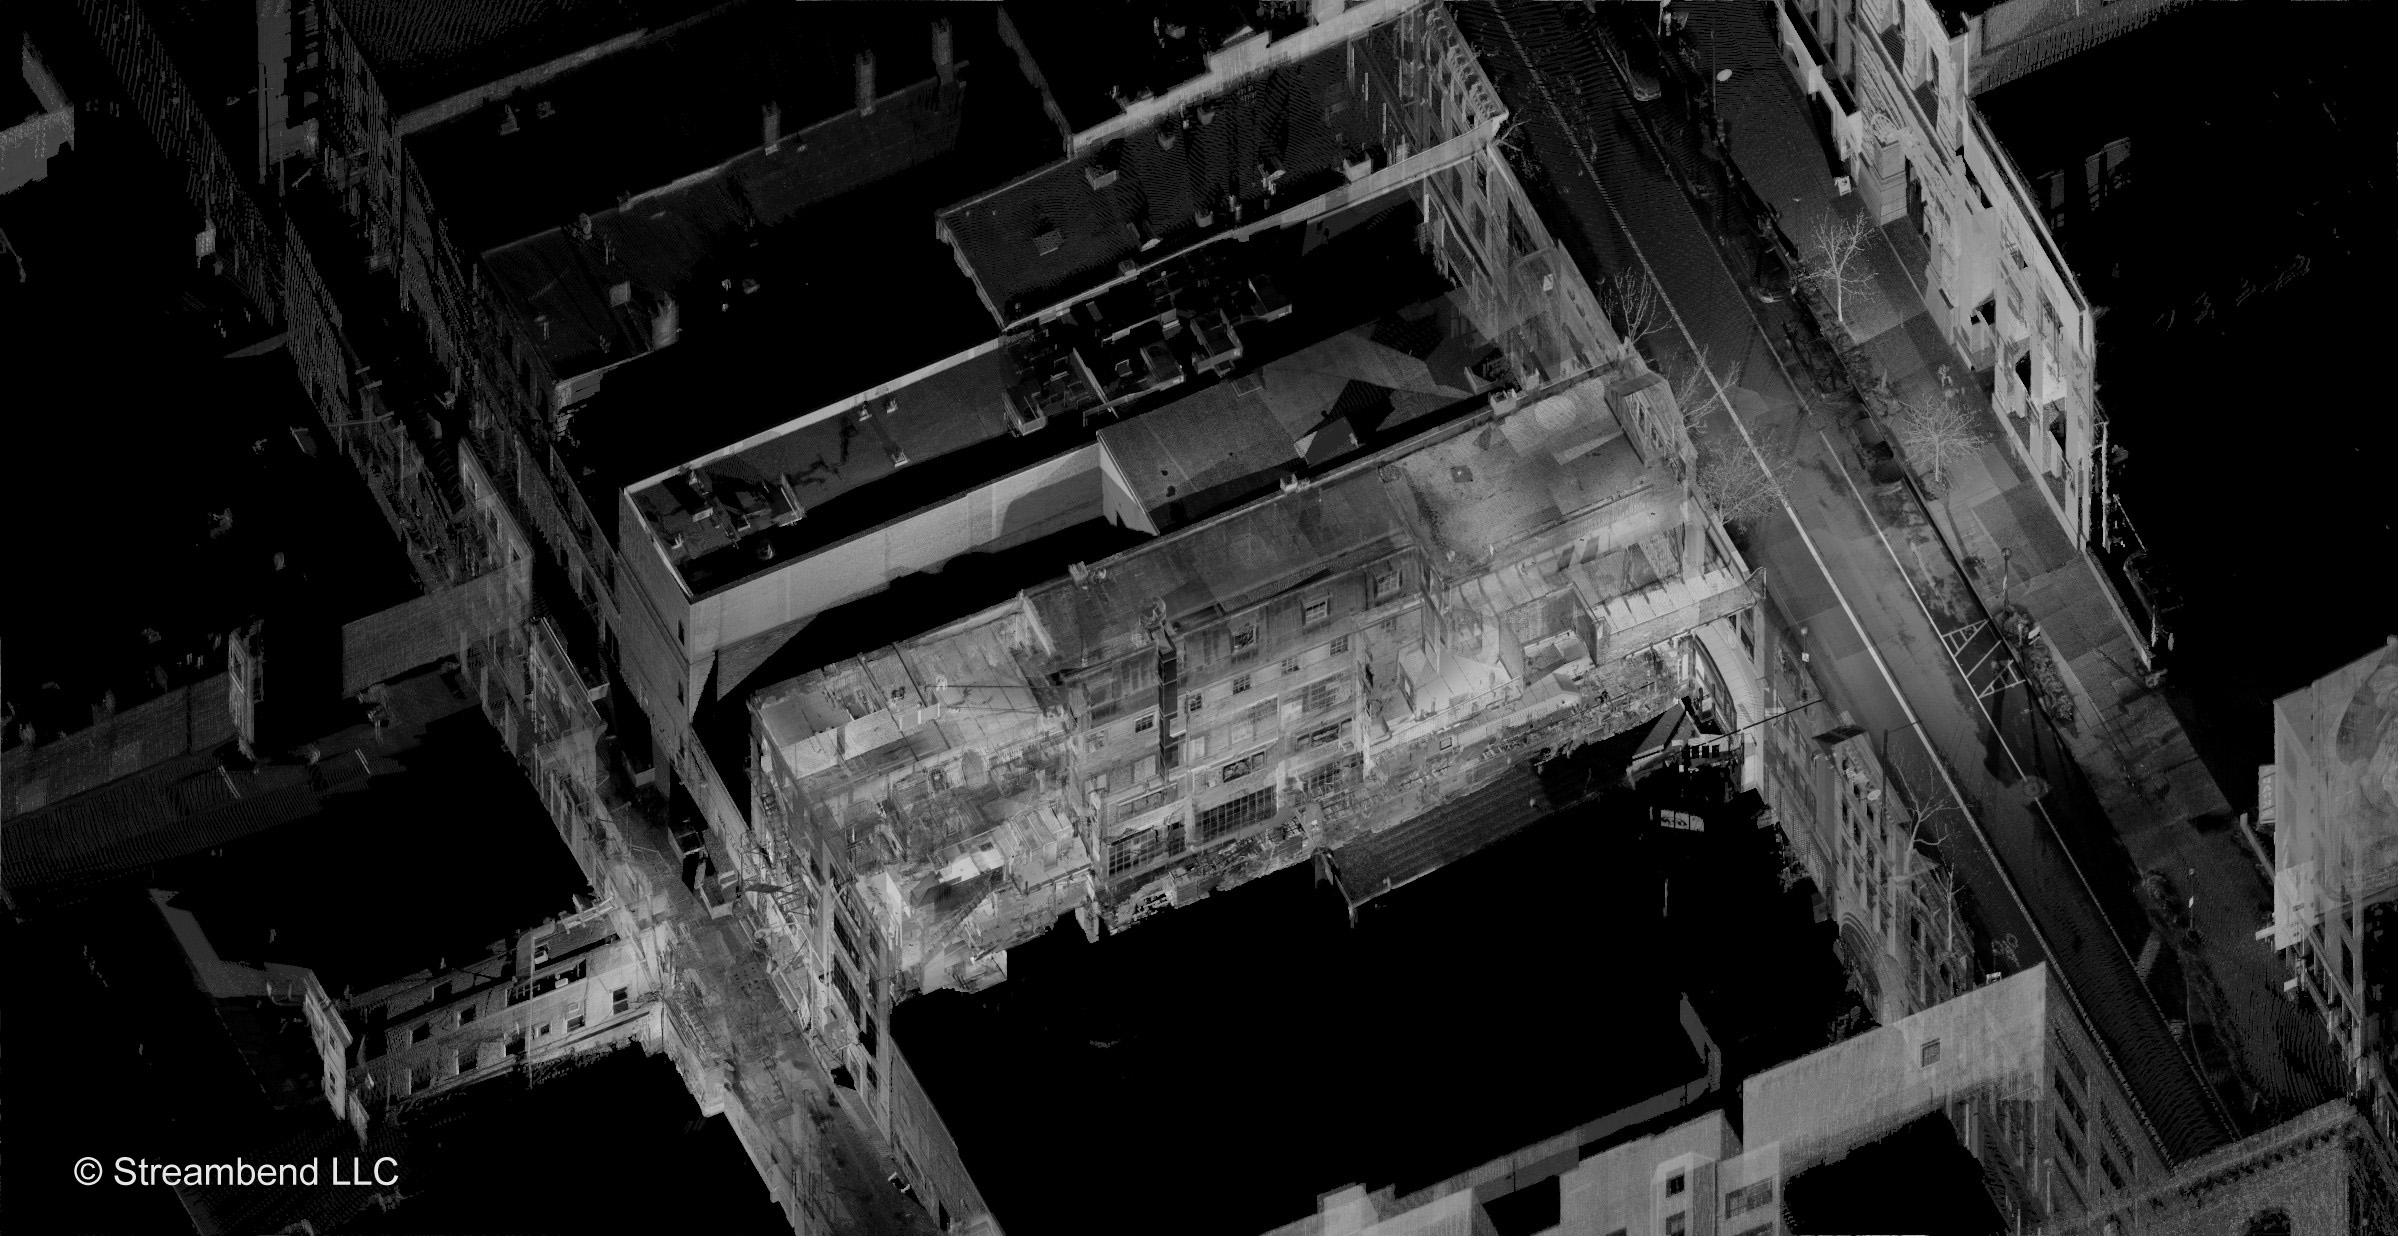
\includegraphics[width=12cm]{faro-scan}
    \caption{Faro 3D scan.}
    \label{fig:faro-scan}
    
\end{figure}

\section{3D Digital Models}

Recreating a real scene with computer graphics is an important topic in today's world and many advancements are being made to create the illusion, for the user, that what he is seeing is real. Many technologies and advancements appeared, like Virtual-Reality, high definition models, photo-realistic rendering and dynamic models. One of the biggest objectives of 3D reconstruction is the possibility of using this technologies to recreate real 3D scenes, making it possible for anyone with a computer or a VR-set to experience this scenes. The number of applications are huge, but the problem remains: how can we save a 3D environment?

In computer graphics, the most common representation is a polygonal mesh. It is composed by a collection of vertices, edges and faces composing a set of polygons that represents a simplification of the original geometry. Because of its flexibility and wide use, graphic cards are specially optimized to render meshes, so models with high detail can be renderer in real-time. Properties of the object, such as color and material, can be added per-vertex or per-face, making it a flexible model to save all the details of the scene. There are also many drawbacks to this representation, for example, the inadequate representation of non-linear surfaces, requiring large high resolution sampling to represent them reliably.

However, it is impossible to get a mesh directly from a 3D scanner, so a simpler model is used instead: the point cloud. A point cloud is a set of points sampled from the surface of the objects, so its level of  detail depend largely on the density of the points. Point clouds can also store extra data pixel-wise, for example, color, normals, intensity or segmentation index.

Because it is such a simple representation, it is very used in robotics and 3D vision, for example, in search and rescue robots, for mapping and navigation, in unmanned vehicles, for road segmentation and in bin-picking robots, for object segmentation. However, it is not adequate for scene reconstruction, because a realistic model requires a huge density of points, which is unfeasible for numerous reasons. To start with, rendering point clouds is slow in modern graphic cards, because the rendering pipeline is not optimized for it, resulting in slow framerate, which then causes a poor experience for the user and unsuitable for VR. Despite new advancements in point-rendering algorithms, capable of rendering point clouds with billion points in commodity hardware \cite{wimmer2006}, it will always be a limiting factor for this model. Also, some of the processing algorithms for point clouds have non-linear time complexity, so point clouds with many points can have long processing times. One of the most wide-spread solutions is to down-sample the point cloud to speed up the algorithms. Finally, large amounts of data are repeated in the point cloud, resulting in redundancy problems and large file sizes. For example, planar surfaces require the same density of points as any complex surface, while in meshes, the density of faces can be adjusted to the gradient of the surface.

These problems are usually solved by performing a triangulation of the point cloud, a process where a mesh is produced. However, this process requires a fine point cloud, that usually require many man-hours of thorough processing, to yield acceptable results. That is why LiDAR Laser scanner is so valuable for 3D reconstruction, as it yields raw point clouds with a better definition than any other technology, requiring less post-processing work in the triangulation process.

\chapter{Experimental Infrastructure}

This chapter describes in detail both the hardware and software used in this project. The hardware - a mobile robot - is described in \cref{section:hardware} and all the software implemented in this robot is described in \cref{section:software}.

% \section{Hardware}
\label{section:hardware}

The hardware used in this work was a mobile 3D scanner called "lemonbot", shown in \cref{fig:lemonbot}. This scanner was developed to perform the acquisitions, and the goal was to build a platform that had minimum interference with the environment (for example, no cables are required), mobile (lightweight and easy to transport) and did not require the presence of the operator. Therefore, the robot was all packed into a tripod which also has a battery capable of powering all the systems. The control is made via a remote connection through the router, which is specially useful to make the repetitive task of acquisitions faster and more agile. 

\begin{figure}[p]
    
    \centering
    \includegraphics[height=20cm]{lemonbot}

    \caption{Lemonbot mobile 3D scanner}
    \label{fig:lemonbot}
\end{figure}

This robot has, in total, seven components: three of which are the essencial components for the acquisitions: the 2D laser scanner, the camera and the pan-tilt unit, or PTU and the other four components form the infrastructure: the minicomputer, the wireless router, the battery pack and finally the tripod. Each of these components are described in detail in the following lines.

\subsubsection{2D Laser Scanner}

One of the objectives of this work is to use different 2D laser scanners to study the performance of the reconstruction and calibration algorithms and to evaluate if not every laser scanner is fit for this application. So, three laser scanners were chosen: the SICK~LMS200, the Hokuyo~UTM30LX and the Hokuyo~URG04. Each of the laser scanners differ in their characteristics, like the size, price, range and error. In \cref{table:laserscanner-characteristics}, all three laser scanners can be compared and in \cref{fig:laserscanners} are shown.

\begin{table}[h]
    \caption{Comparison of the three laser scanners used, based on the data provided by the manufacturers.}

    \begin{tabu}{@{}>{\bfseries}X[l,m] X[c] X[c] X[c]@{}}
        \toprule

            & SICK LMS~100
            & Hokuyo UTM~30LX
            & Hokuyo URG04 \\
        \toprule

        \everyrow{\midrule}

        Aperture angle &
            \SI{270}{\degree} &
            \SI{270}{\degree} &
            \SI{240}{\degree} \\
        
        
        Angular resolution &
            \SI{0.25}{\degree} &
            \SI{0.25}{\degree} &
            \SI{0.36}{\degree} \\
        
        
        Scanning frequency &
            \SI{10}{\hertz} &
            \SI{40}{\hertz} &
            \SI{10}{\hertz} \\
        

        Maximum range &
            \SI{20}{\meter}  &
            \SI{30}{\meter}  &
            \SI{5.6}{\meter} \\
        

        Systematic error &
            \SI{+-40}{\milli\meter} &
            not available &
            not available \\
        
        
        Statistical error &
            \SI{20}{\milli\meter} &
            \SI{30}{\milli\meter} &
            \SI{30}{\milli\meter} \\
        

        Dimensions (\si{\milli\meter^3}) &
            \num{152x102x106} &
            \num{60x60x87} &
            \num{60x60x87} \\
        

        Weight &
            \SI{1100}{\gram} &
            \SI{370}{\gram} &
            \SI{160}{\gram} \\
        
        \everyrow{}

        Power consumption &
            \SI{<12}{\watt} &
            \SI{8.4}{\watt} &
            \SI{2.5}{\watt} \\

        \bottomrule
    \end{tabu}

    \label{table:laserscanner-characteristics}
\end{table}


\begin{figure}[h]
    
    \centering
    \begin{subfigure}{0.3\textwidth}
        \centering
        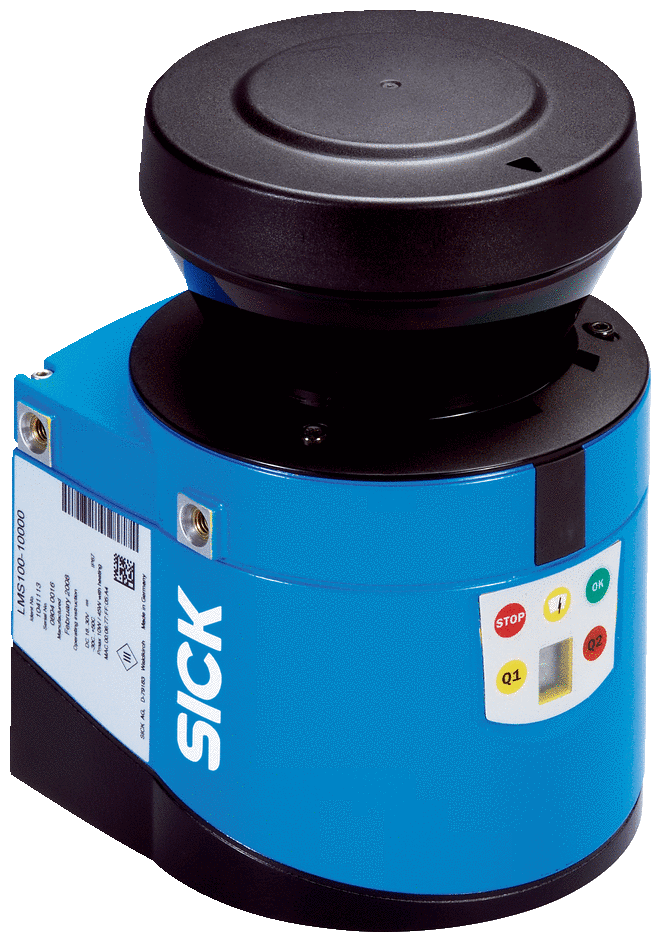
\includegraphics[height=4cm]{sick-lms100}
        \caption{SICK LMS100}
        \label{fig:sick-lms100}
    \end{subfigure}%
    \begin{subfigure}{0.3\textwidth}
        \centering
        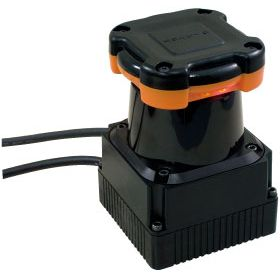
\includegraphics[height=4cm]{hokuyo-utm30lx}
        \caption{Hokuyo UTM30LX}
        \label{fig:hokuyo-utm30lx}
    \end{subfigure}%
    \begin{subfigure}{0.3\textwidth}
        \centering
        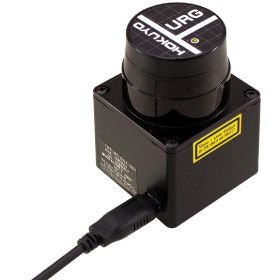
\includegraphics[height=4cm]{hokuyo-urg04}
        \caption{Hokuyo URG04}
        \label{fig:hokuyo-urg04}
    \end{subfigure}

    \caption{Laser scanners used.}
    \label{fig:laserscanners}

\end{figure}

\subsubsection{Camera}

The camera used in this work was a PointGrey Flea3 FL3-GE-28S4 Camera (\cref{fig:pointgrey-flea3}), which is extensively used in industrial and traffic applications. The high quality of the images, the programming interface and it's compact size and weight makes it perfect for computer vision applications in industrial environment. The most relevant characteristics are represented on the \cref{table:pointgrey-flea3-characteristics}.

\begin{figure}[h]
    \centering
    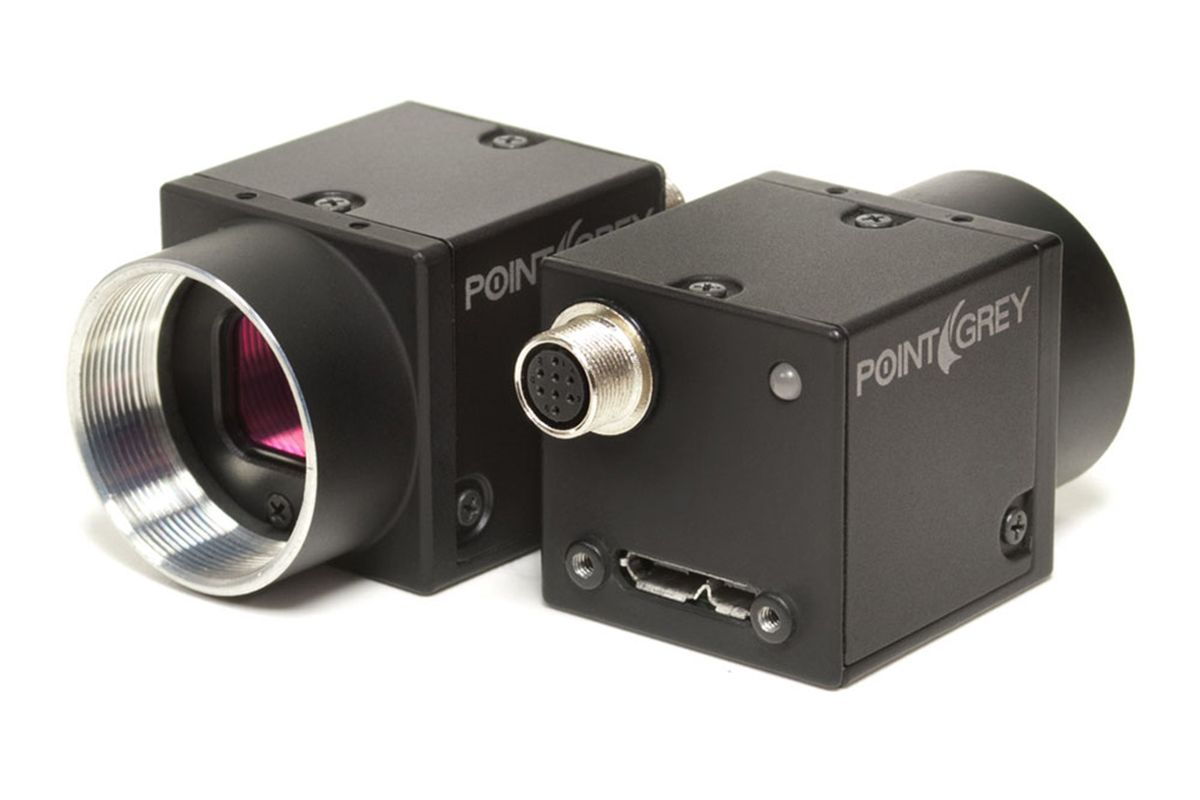
\includegraphics[width=0.5\textwidth]{pointgrey-flea3}
    \caption{PointGrey Flea3 FL3-GE-28S4}
    \label{fig:pointgrey-flea3}
\end{figure}

\begin{table}[h]

    \caption{Characteristics of the PointGrey Flea3 FL3-GE-28S4 Camera}

    \centering
    \begin{tabu} spread 0.2\textwidth {>{\bfseries}X[l] X[r]}
        \toprule

        Resolution  & $1920 \times 1448$    \\
        Framerate   & 15 fps                \\
        Pixels      & \SI{2.8}{\mega P}     \\
        Color       & Yes                   \\
        Interface   & GigE Vision           \\
        Power       & \SIrange{12}{24}{\volt} \\
        Dimensions  & \SI{29 x 29 x 30}{\milli\meter} \\
        \bottomrule
    \end{tabu}

    \label{table:pointgrey-flea3-characteristics}

\end{table}

\subsubsection{Pan Tilt Unit}

Both the laser and camera are placed on top of a pan and tilt unit for their movement. The selected PTU was the FLIR PTU-D46 (\cref{figure:ptu-d46}), which is a compact and light module with the characteristics shown in \cref{table:ptu-characteristics}.


\begin{table}[h]
    \caption{FLIR PTU-D46 characteristics.}

    \centering
    \begin{tabu} spread 0.15\textwidth {>{\bfseries}X[l] X[r]}
        \toprule
        Pan range & \SI{+-159}{\degree} \\
        Tilt range & \SIrange{-47}{+31}{\degree} \\
        Maximum payload weight & \SI{4}{\kilo\gram} \\
        Angular resolution & \SI{0.0032}{\degree} \\
        Communication & serial interface \\
        Size & small \\
        \bottomrule
    \end{tabu}

    \label{table:ptu-characteristics}
\end{table}

\begin{figure}[h]
    \centering
    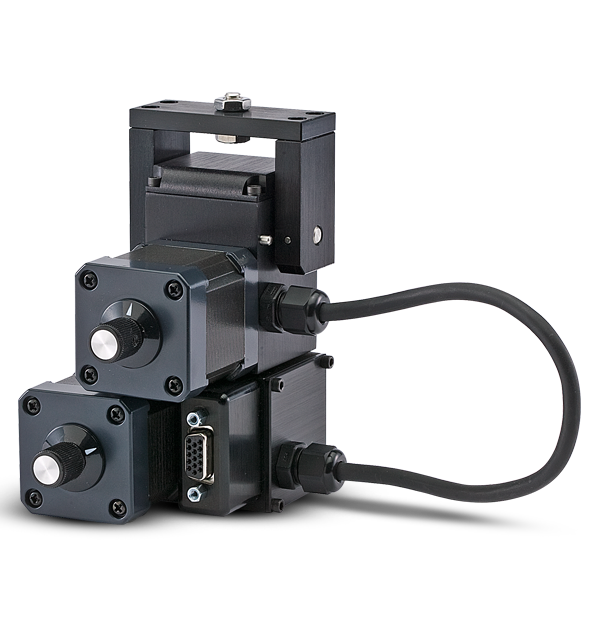
\includegraphics[width=0.5\textwidth]{ptu-d46}
    \caption{FLIR PTU-D46}
    \label{figure:ptu-d46}
\end{figure}

\section{Software}
\label{section:software}

This section describes the software used in this work. In general, two different applications were developed. One application was the software that constitutes the mobile 3D scanner, which was developed in a framework called Robot Operating System, described in \cref{section:ros}. The other one is the software used to process the data recorded by the 3D scanner, which is described in \cref{section:processing-application}.

\subsection{Robot Operating System}
\label{section:ros}

Robot Operating System, or ROS, is a software architecture for robot development, providing a collection of tools, libraries and conventions to simplify the development of complex robotic systems. It was originally created at stanford University in the mid-2000s and new is widely adopted as the standard framework for robotics by most research communities.

Its design principles follow the one of a distributed system. In ROS, a system is composed by multiple nodes that have just one task and communicate between them by message passing. To achieve this, ROS, in its core, has the infrastructure responsible for the:

\begin{description}
    \item[Orchestration]. ROS runs, stops and monitors all nodes, so in the case of failure, for example, ROS is capable of restarting the node.
    \item[Communication]. ROS provides both the pipelining to distribute messages as well as the standard serialization specification.
    \item[Configuration]. ROS provides a key-value store for parameters that are accessible for nodes. These parameters can be specified when the node is created and also changed dynamically at runtime.
    \item[Discovery]. Each node in the environment can inspect it, such as finding other nodes and finding topics.
\end{description}

This architecture has many advantages, such as:

\begin{description}
    \item[Fault-tolerant]. A failure in one node does not affect other nodes, so there is not a overall system crash, unlike monolithic systems. Usually, because errors are transitive and not very frequent, a restart-on-failure policy is used to keep the downtime low.
    \item[More generic]. Because each node has a single responsibility, they tend to be more generic and detached to a single project, so integration in a new project can be easy. This is fundamental to reduce the need to "reinvent the wheel", therefore reducing the development cost and time of this complex systems.
    \item[Easier to develop]. Each component can be developed be separate developers, with different languages and independent release cycles, because they do not have any dependency between each over and only a message specification needs to be agreed on between developer teams, making collaborative development possible. Debugging is also easier, because each node can be unit-tested separated from the "real environment".
    \item[Large Community]. ROS is open source, which incentivises different research groups to share packages. Also, ROS is widely adopted so multiple packages for numerous tasks are already programmed, and can be integrated easily into new systems. One of this examples are drivers, which almost never require to be developed, because most robotic hardware already has a developed driver.
\end{description}

ROS is split into 3 levels, according to~\cite{fernandez_2015}: the \textit{filesystem} level, the \textit{the computational graph} level and the \textit{community} level. Each level is composed of several core components, that make the whole system work, as seen in \cref{figure:ros_overview}. Some components that were required for this work are explained next.

\begin{figure}[h]
    \label{figure:ros_overview}
        
        \caption{ROS architecture overview}
    
        \tikzstyle{ros_level}=[rectangle, draw, text centered, thick, text width=8em, rounded corners, font=\bfseries]
        \tikzstyle{level}=[rectangle, draw, font=\bfseries, thick, rounded corners, inner xsep=0.5cm]
        \tikzstyle{component}=[rectangle, draw, text width=9em]
    
    
        \centering
        \begin{tikzpicture}[scale=0.9]
            
            \node[ros_level] (ROS) {ROS};
            \coordinate[below=0.4cm of ROS] (aux_node1);
            \node[level, below=0.6cm of aux_node1] (computational_graph) {Computational Graph};
            \node[level, left=1.7cm of computational_graph] (filesystem) {Filesystem};
            \node[level, right=1cm of computational_graph] (community) {Community};
    
            \draw[->] (ROS) -- (aux_node1) -- (computational_graph.north);
            \draw[->] (ROS) -- (aux_node1) -| (filesystem.north);
            \draw[->] (ROS) -- (aux_node1) -| (community);
    
            \coordinate[below=of filesystem.west, xshift=0.5cm] (aux_node2);
            \coordinate[below=of computational_graph.west, xshift=0.5cm] (aux_node3);
            \coordinate[below=of community.west, xshift=0.5cm] (aux_node4);
    
            \node[component, anchor=west, yshift=0cm] (meta_packages) at (aux_node2) {Meta Packages};
            \node[component, anchor=west, yshift=-0.8cm] (packages) at (aux_node2) {Packages};
            \draw[->] (filesystem.west) -- ++(-0.2cm, 0) |- (meta_packages.west);
            \draw[->] (filesystem.west) -- ++(-0.2cm, 0) |- (packages.west);
    
            \node[component, anchor=west, yshift=0cm] (nodes) at (aux_node3) {Nodes};
            \node[component, anchor=west, yshift=-0.8cm] (master) at (aux_node3) {Master};
            \node[component, anchor=west, yshift=-1.6cm] (param_server) at (aux_node3) {Parameter Server};
            \node[component, anchor=west, yshift=-2.4cm] (messages) at (aux_node3) {Messages};
            \node[component, anchor=west, yshift=-3.2cm] (topics) at (aux_node3) {Topics};
            \node[component, anchor=west, yshift=-4.0cm] (services) at (aux_node3) {Services};
            \node[component, anchor=west, yshift=-4.8cm] (bags) at (aux_node3) {Bags};
            \draw[->] (computational_graph.west) -- ++(-0.2cm, 0) |- (nodes.west);
            \draw[->] (computational_graph.west) -- ++(-0.2cm, 0) |- (master.west);
            \draw[->] (computational_graph.west) -- ++(-0.2cm, 0) |- (param_server.west);
            \draw[->] (computational_graph.west) -- ++(-0.2cm, 0) |- (messages.west);
            \draw[->] (computational_graph.west) -- ++(-0.2cm, 0) |- (topics.west);
            \draw[->] (computational_graph.west) -- ++(-0.2cm, 0) |- (services.west);
            \draw[->] (computational_graph.west) -- ++(-0.2cm, 0) |- (bags.west);
    
            \node[component, anchor=west, yshift=0cm] (distributions) at (aux_node4) {Distributions};
            \node[component, anchor=west, yshift=-0.8cm] (repositories) at (aux_node4) {Repositories};
            \node[component, anchor=west, yshift=-1.6cm] (ros_wiki) at (aux_node4) {ROS Wiki};
            \node[component, anchor=west, yshift=-2.4cm] (bug_ticket_system) at (aux_node4) {Bug Ticket System};
            \node[component, anchor=west, yshift=-3.2cm] (mailing_lists) at (aux_node4) {Mailing Lists};
            \node[component, anchor=west, yshift=-4.0cm] (ros_answers) at (aux_node4) {Ros Answers};
            \node[component, anchor=west, yshift=-4.8cm] (blog) at (aux_node4) {Blog};
            \draw[->] (community.west) -- ++(-0.2cm, 0) |- (distributions.west);
            \draw[->] (community.west) -- ++(-0.2cm, 0) |- (repositories.west);
            \draw[->] (community.west) -- ++(-0.2cm, 0) |- (ros_wiki.west);
            \draw[->] (community.west) -- ++(-0.2cm, 0) |- (bug_ticket_system.west);
            \draw[->] (community.west) -- ++(-0.2cm, 0) |- (mailing_lists.west);
            \draw[->] (community.west) -- ++(-0.2cm, 0) |- (ros_answers.west);
            \draw[->] (community.west) -- ++(-0.2cm, 0) |- (blog.west);
    
        \end{tikzpicture}
    
    \end{figure}

\subsubsection{Messages}

Messages are the communication element and are just structures of data composed by primitive types such as integers, floating point numbers, strings and other messages. All messages follows a schema, which is required to encode and decode the message. Messages are serialized in a binary format before and after the exchange, so messages are small and efficient. Moreover, all messages have a header, which contains a timestamp and the source of the message. 

\subsubsection{Topics}

Topics are named buses over which nodes exchange messages. Topics follow the publisher/subscriber paradigm, so nodes can both subscribe to receive messages or publish messages to the topics. The exchange of data is done anonymously, so nodes are not aware which nodes are publishing or subscribing to a topic. This way of exchanging data is well suited for streaming data, such as sensor data.

\subsubsection{Launch Files}

Launch files are xml files that describe the steps to launch multiple node, as well as setting parameters. Launch files also support composition, so a launch file can invoque other launch files. Launch files were used in this project extensively, to launch the drivers of the mobile robot and to launch the acquisitions.

\subsubsection{Bags}

A bag is a file format for storing ROS messages, and have a myriad of tools to store, process, visualize and analyze them. During runtime, bags can be used to store the messages published in multiple topics, so data can be analysed later. Also, messages in bag files can be republished back into the system for testing or visualization purposes.

In this work, bag files played a very important role, as they were responsible to store the sensor data and also the transformation graph of the 3D scanner.

\subsubsection{RViz}

RViz is a 3D visualizer for ROS for displaying sensor data, like laser scans and point clouds, and the representation of the robot state, like the position of the coordinate frames and the joints. RViz can be a indispensable debug tool, for example, by comparing the real environment with the displayed environment shown in RViz.

\subsubsection{TF}

TF is a package that keeps track of multiple coordinate frames and maintains the relationship between coordinate frames in a tree structure, called the transformation graph. This transformation graph can be queried to obtain the transformation between two frames at any point in time. Also, tf can work in distributed systems, just like ROS, so any node can publish transformations and the transformations can be obtained in any node. TF is also responsible to interpolate between the discrete transformations and handle transformations with different sampling rates.

\subsubsection{URDF}

Unified Robot Description Format, or URDF, is a format to represent a robot model, like the joints and links configuration and the geometry of the joints. This file is loaded at runtime and the transformations are published according to the joint state. 


\subsection{Processing Application}
\label{section:processing-application}

This application required a wide spectrum of libraries, frameworks, file formats and graphical programs, which are described next.

\subsubsection{Libraries and Frameworks}

The software developed in this work that implements the processing algorithms was done using the Python programming language and some libraries to provide both data structures and common algorithms. Both the language and libraries are described next.

\begin{description}
    \item[Python] is a general purpose programming language that become popular for its syntax and small learning curve. It is also the defacto language for science, along with MATLAB. However, inlike MATLAB, it is s open source, has large community and has plenty of libraries that provide many algorithms and efficient data structures. Also, it is a dynamic language, which facilitates the process of testing and debugging the code developed.

    \item[Numpy] is a library that contains an implementation of $nd$-arrays, as well as algorithms to manipulate them. This library was fundamental for this work to store and process the point data. The main advantage of this library is that it is implemented in compiled languages like C and Fortran to implement high performance and optimized data structures and algorithms, available through a clean interface in Python.

    \item[Pandas] is a library that provides a fundamental data structure which was extensively used in this work: the DataFrame. DataFrames store data in columns, which is perfect to store tabular data. This is a common way to store point information, because point clouds are, fundamentally, tables, where each property are stored as a column, like $x$, $y$, $z$ for position and $r$, $g$, $b$ for color. Also, because it relies on numpy arrays to store the data, it is still very high performance.

    \item[PIL], or Python Image Library, is a library for image loading and manipulation, and was used to read and write the images recorded by the camera. 
    
    \item[Jupyter] provides an interactive interfaces, called Jupyter notebooks, which provides interactive documents with embedded code. This notebooks are extremely useful and were used to document and explore the code that was used in this work.

\end{description}

\subsubsection{File Formats}

\begin{description}
    
    \item[AVRO] is a binary data serialization format that is user to store collections of structured data. This format was chosen to store the laserscans and the image metadata. AVRO relies on schemas, which describe the data in the file is stored with the data. Therefore, an AVRO file is self-describing and data can be read and write without much overhead. Moreover, this format is implemented in Python and has numerous tools for inspection and conversion of the data.

    \item[PLY], or Polygon File Format is one of the most used and supported file formats to store three dimensional data, like point clouds and meshes. It was originally developed and used in the Stanford University to store data from 3D scanners. It supports a wide number of properties, like color, transparency, surface normals and texture coordinates. It also supports the storage of custom properties, which were required for this work, for example in the segmentation for the calibration. Moreover, it supports binary encoding, so files are small and fast to read and write.

    \item[JPEG] is a commonly used format for images and was used to store the recorded images.

    \item[YAML] is an human readable format that was used to store the parameters of the acquisitions, suck as the the extrinsic calibration of the sensors. The advantage of this format is that files are very easy to read and modify by the user.

\end{description}

\subsubsection{Graphical Software}

\begin{description}
    
    \item[CloudCompare] is a software to render, process and manipulate 3d point clouds. It includes many algorithms, like point cloud registration, re-sampling, handling scalar fields, and automatic or interactive segmentation. It can also render point clouds using different shaders and support point cloud decimation, which is a technique that allows manipulation of large point clouds without a decrease in performance. A screenshot of this software can be seen in \cref{fig:cloud-compare}.

\end{description}

\begin{figure}[h]
    \centering
    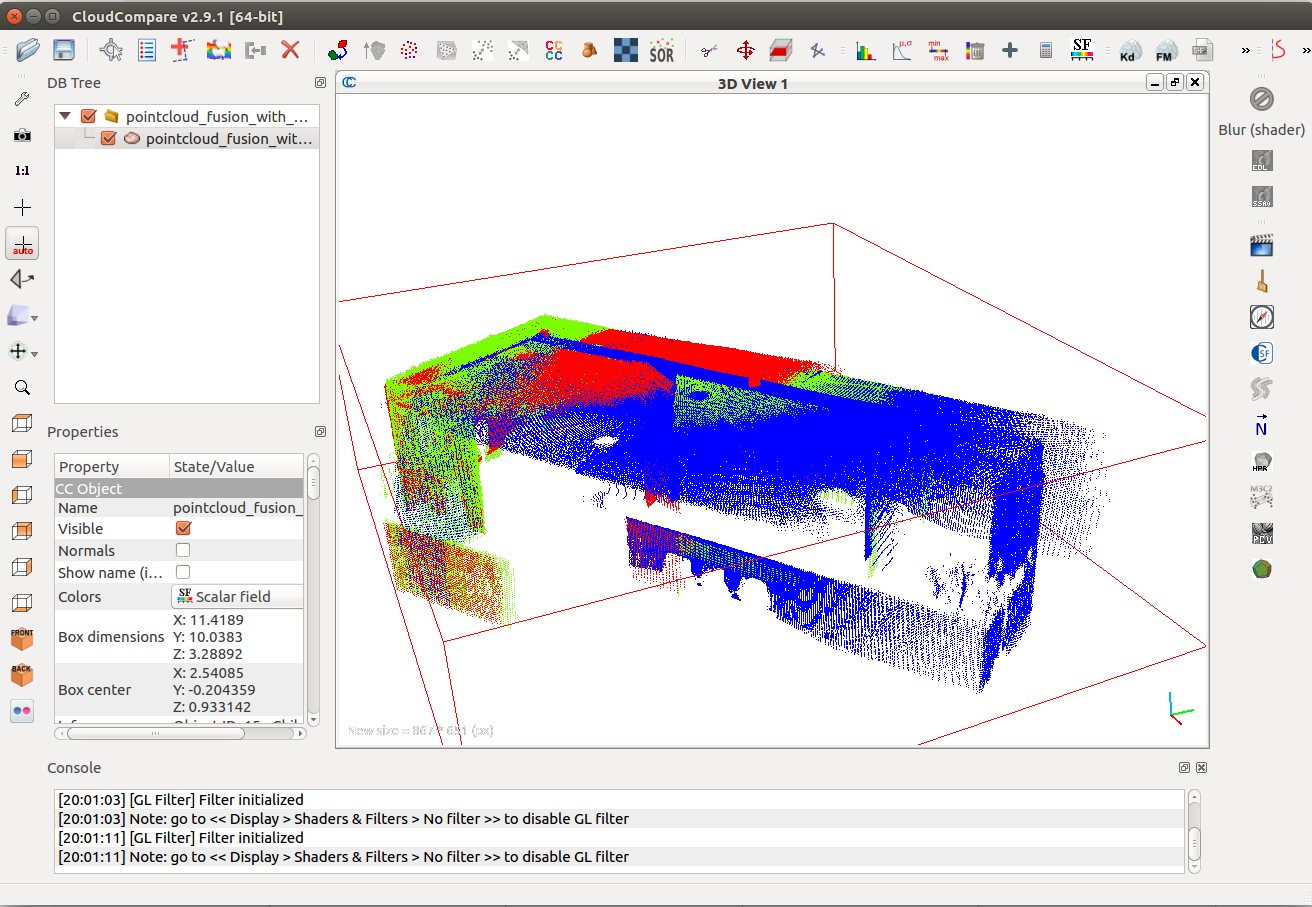
\includegraphics[width=15cm]{cloudcompare}
    \caption{Cloud Compare screenshot.}
    \label{fig:cloud-compare}
\end{figure}


\chapter{Methodology for 3D Scene Acquisition}
\label{chapter:scene_capture_methodology}

This chapter describes the concepts and methodology around a capture of a scene. This methodology is split into two levels: the acquisition and the capture level. An acquisition is a collection of sensor data recorded from a specific position of the scene and a capture is a collection of acquisitions taken from the scene scene, but from different positions.

The reason behind these two level has to be because there is limited information about the scene in each acquisition. These limitations are the occlusion of different parts of the scene by objects, the hardware limitation of sensors, like the small aperture angle of the laser scanner or the field of view of the camera, and the environment factors, for example, the lightning conditions and the reflectivity of the object's surfaces. This effects are show in \cref{figure:limitations-single-acquisition}. To overcome these limitations, multiple acquisitions required, however, this also comes with some challenges, for example, how to merge all the acquisitions and how to handle the redundant data.

So, acquisitions and captures are different levels and each one has a different method and objectives. In an acquisition level, the focus is on how to operate the scanner and define how the data is recorded. In a capture level, the focus is on how to plan multiple acquisitions so a good reconstruction is possible. In the following sections, both acquisitions and captures are further explained.

\begin{figure}
    
    \tikzset{
        camera/.pic = {
            \draw (-0.08, -0.08) rectangle (0.08, -0.25);
            \draw (-0.06, -0.08) rectangle (0.06, 0);
        },
        laser/.pic = {
            \draw (0, 0) circle (0.08);
            \draw (-0.08, -0.08) rectangle (0.08, 0.08);
            
            \draw[-stealth] (0,0) -- (0, 0.40) node[anchor=east, scale=0.5] {$x$};
            \draw[-stealth] (0,0) -- (-0.40, 0) node[anchor=east, scale=0.5] {$y$};
        }
    }

    \centering
    \begin{subfigure}[t]{0.3\textwidth}
        \centering
        \begin{tikzpicture}
            \draw (0,0) rectangle (4,4);
    
            \coordinate (camera) at (1,1);
    
            \node[scale=0.5, anchor=north west] at (camera) {camera};
    
            \draw (2, 2) rectangle +(1,1);
    
            \node[scale=0.5] at (2.5,2.5) {object}; 
    
            \draw (camera) pic[rotate=-45] {camera};
            \draw[-stealth, rotate=-45, very thin] (camera) -- +(0, 0.6) node[scale=0.5, anchor=south west] {$z$};
    
            \draw[very thin, dashed] (camera) -- (1.6, 4);
            \draw[very thin, dashed] (camera) -- (4, 1.6);

            \draw[very thin, dotted] (camera) -- (2.5,4);
            \draw[very thin, dotted] (camera) -- (4, 2.5);
    
            \pattern[pattern=north east lines] (2.5,4)--(4,4)--(4,2.5)--(3,2) -- (3,3) -- (2,3) -- cycle;

        \end{tikzpicture}

        \caption{Occlusion in a camera}
    \end{subfigure}
    \begin{subfigure}[t]{0.3\textwidth}
        \centering
        \begin{tikzpicture}
            \draw (0,0) rectangle (4,4);

            \coordinate (laser) at (1,1);

            \draw (laser) pic {laser};

            \node[anchor=west, scale=0.5, xshift=5] at (laser) {l.s.};

            \draw[very thin, dashed] (laser) -- (0,0.2);
            \draw[very thin, dashed] (laser) -- (2.2, 0);

            \draw[very thin, dotted] (laser) -- (4,3);
            \draw[very thin, dotted] (laser) -- (4, 0);

            \draw (2.5,0.5) rectangle (2.8,2);

            \node[scale=0.5, rotate=90] at (2.65, 1.21) {wall};

            \pattern[pattern=north east lines] (4,0) -- (4,3) -- (2.5, 2) -- (2.8,2) -- (2.8, 0.5)
                -- (2.5, 0.5) -- cycle;
    
        \end{tikzpicture}

        \caption{Occlusion in a laser scanner}
    \end{subfigure}
    \begin{subfigure}[t]{0.3\textwidth}
        \centering
        \begin{tikzpicture}
            \draw (0,0) rectangle (4,4);

            \coordinate (camera) at (1,2);
            \draw (camera) pic[rotate=-90] {camera};
            \draw[-stealth, very thin] (camera) -- +(0.6, 0) node[scale=0.5, anchor=south west] {$z$};

            \foreach \a/\c in {1/0.8,2/1.4,3/2} {
                \draw[very thin, dashed, dash pattern=on 2*\a off 2*\a] (camera) -- (4, 2 + \c);
                \draw[very thin, dashed, dash pattern=on 2*\a off 2*\a] (camera) -- (4, 2 - \c)
                    node[pos=0.8, above, scale=0.4] {$f_{\a}$};
            };

        \end{tikzpicture}

        \caption{Different focal points of a camera}
    \end{subfigure}
    
    \begin{subfigure}[t]{0.3\textwidth}
        \centering
        \begin{tikzpicture}
            \draw (0,0) rectangle (4,4);
            \clip (0,0) rectangle (4,4);

            \foreach \a/\c in {180/0, 225/1, 270/2} {
                \draw[very thin, dashed] (0, 1.5-\c) -- (2,1.5) node[pos=0.4, scale=0.4, sloped, anchor=south] {$r = \SI{\a}{\degree}$} -- (4, 1.5-\c);
            };

            \draw[ultra thin, dashdotted] (2, 1.5) -- +(0, 3);


            \draw (2,1.5) pic {laser};
    
        \end{tikzpicture}

        \caption{Radial aperture of a laser}
    \end{subfigure}
    \begin{subfigure}[t]{0.3\textwidth}
        \centering
        \begin{tikzpicture}
            \draw (0,0) rectangle (4,4);
            \clip (0,0) rectangle (4,4);
            
            \coordinate (laser) at (1,1);
            \draw (laser) pic {laser};
            \node[anchor=west, scale=0.5, xshift=5] at (laser) {l.s.};

            \draw[thin, dashed] (laser) -- (0,0);
            \draw[thin, dashed] (laser) -- (2, 0);
            
            \fill[pattern=north east lines] (2, 3.3) -- (2, 2.5) arc (45+11:45-11:1.8) -- (2.5, 2) -- (3.3, 2) arc (45-21.2:45+21.2:2.5) -- cycle;
            \draw (2, 2) rectangle (3.5, 3.5);

            \begin{scope}
                \clip (0,0) rectangle (4,4);
                \draw[thin, dashed, dash pattern=on 2pt off 2pt] (laser) circle (1.8);
                
                \draw[thin, dashed, dash pattern=on 5pt off 5pt] (laser) circle (2.5);                
            \end{scope}

            \node[scale=0.5, anchor=east] at (2.8, 1) {$r_1$};
            \node[scale=0.5, anchor=east] at (3.5, 1) {$r_2$};

        \end{tikzpicture}

        \caption{Range limitations}
    \end{subfigure}
    \begin{subfigure}[t]{0.3\textwidth}
        \centering
        \begin{tikzpicture}
            \draw (0,0) rectangle (4,4);
            \clip (0,0) rectangle (4,4);

            \coordinate (laser) at (1,1);
            \draw (laser) pic {laser};
            \node[anchor=west, scale=0.5, xshift=5] at (laser) {l.s.};


            \foreach \a in {0, 5, ..., 180} {
                \def\x{{cos(\a)}};
                \def\y{{sin(\a)}};
                \draw[dashed] ($(laser) + 0.6*(\x, \y)$) -- ($(laser) + 5*(\x, \y)$);
            };

            \draw[fill=white, draw=black] (1, 3) rectangle ++(0.7,0.7)
                node[midway, scale=0.5] {obj. 1};

            \draw[fill=white, draw=black] (2, 1.5) rectangle ++(0.7, 0.7)
                node[midway, scale=0.5] {obj. 2};

        \end{tikzpicture}

        \caption{Radial resolution}
    \end{subfigure}

    \caption{Limitations of a single acquisition}

\end{figure}

\section{Acquisition}
\label{section:acquisition}

An acquisition is a collection of sensor data (laser scans and images) collected by the sensors in the scanner. Both sensors sample only a small subset of the whole environment: the laser scans only have points from a planar region of the space and cameras are limited by their focal length. To overcome this limitation, both sensors are moved to different poses in space to cover a wider space. In this case, the cause of movement of the sensors is the movement of the joints of the PTU. 

\subsection{Movement Programming}

To program the motion of the PTU joints, a list of waypoints in pan and tilt are defined and the joints move from waypoint to waypoint. The waypoints are defined in a grid in the joint-space and the movement between waypoints is the one that defines the shortest path possible and most of the movement is done in pan. So, each acquisition is parameterized with the following parameters: the range (minimum and maximum angle) of pan/tilt, the speed of each joint and the number of waypoints in pan/tilt. An example of this parameterization can be seen in \cref{figure:joint-movement}.

Once the movement of the scanner was defined, the next step is to define when to record the laser scans and the images, according to it. Because of the nature of both sensors, it was established that laser scans are captured continuously during the pan movement between the waypoints and images are captured at every waypoint.

\begin{figure}[h]

    \centering
    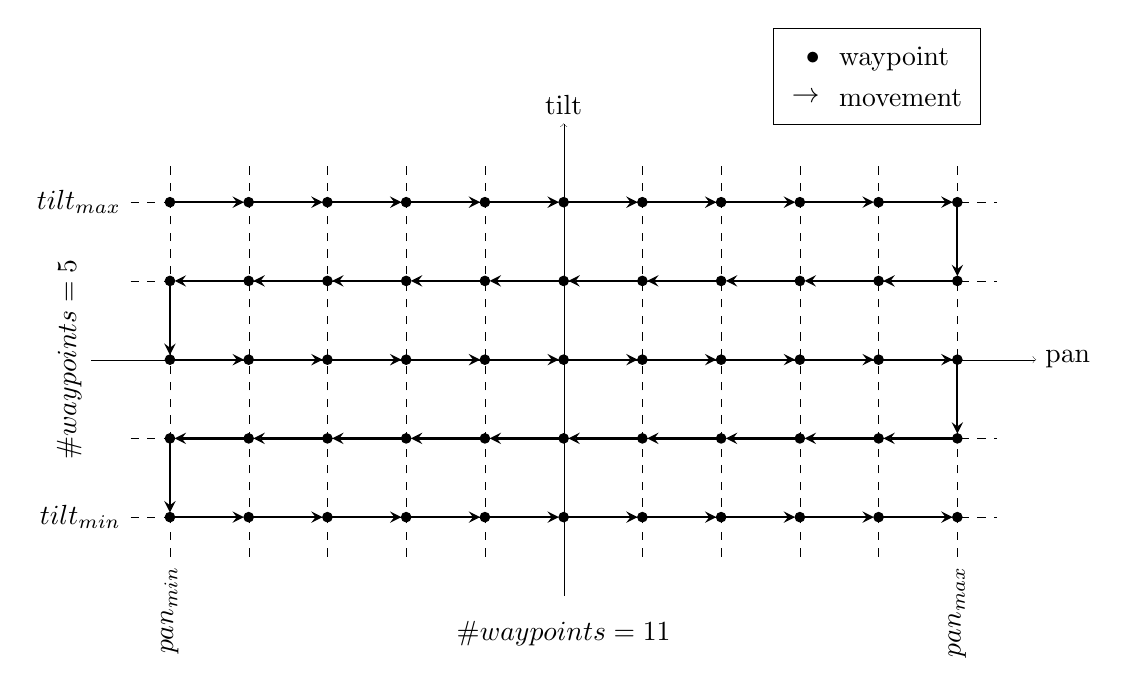
\begin{tikzpicture}

        \draw[->, ultra thin] (-6, 0) -- (6, 0) node[right] {pan};
        \draw[->, ultra thin] (0, -3) -- (0, 3) node[above] {tilt};

        \draw[step=1, ultra thin, dashed] (-5.5, -2.5) grid (5.5, 2.5);

        \foreach \x in {-5,...,5}
            \foreach \y in {-2,...,2}
                \draw[fill=black] (\x, \y) circle (0.06);
        
        \foreach \x in {-5,...,4}
            \foreach \y in {-2,...,2}
                \ifthenelse{\isodd{\y}}{
                    \draw[stealth-, shorten <=0.06cm, thick] (\x, \y) -- (\x+1, \y);  
                }{
                    \draw[-stealth, shorten >=0.06cm, thick] (\x, \y) -- (\x+1, \y);
                };

        \foreach \y in {2,...,-1}
            \ifthenelse{\isodd{\y}}{
                \draw[-stealth, shorten >=0.06cm, thick] (-5, \y) -- (-5, \y - 1);
            }{
                \draw[-stealth, shorten >=0.06cm, thick] (5, \y) -- (5, \y - 1);
            };

        
        \node[anchor=east] at (-5.5, -2) {$tilt_{min}$};
        \node[anchor=east] at (-5.5, 2) {$tilt_{max}$};
        \node[anchor=south, rotate=90] at (-6, 0) {$\#waypoints = 5$};

        \node[anchor=east, rotate=90] at (-5, -2.5) {$pan_{min}$};
        \node[anchor=east, rotate=90] at (5, -2.5) {$pan_{max}$};
        \node[anchor=north] at (0, -3.2) {$\#waypoints=11$};
            
        \matrix[draw, above left, xshift=-1.5cm, yshift=-0.5cm] at (current bounding box.north east) {
            \node[label=right:waypoint] {$\bullet$}; \\
            \node[label=right:movement] {$\rightarrow$}; \\
        };

    \end{tikzpicture}

    \caption{Waypoints and movements in the pan/tilt joint space.}

\label{figure:joint-movement}
\end{figure}


\subsection{Parameterization Considerations}

This methodology has the numerous implications. First, the pan and tilt range is only limited by the PTU capabilities, but it beneficial to use the maximum range possible, in order to get as much data as possible. In this work, most data collected is redundant, for example if multiple tilt angles are used, however this improves the final reconstruction by increasing the density of the point cloud.

Second, the number of laser scans recorded is going to depend on the pan speed and the frequency of scanning of the 2D laser scanner. So, it is expected that a laser scanner with a lower scanning frequency to require a slower speed compared to a faster one, to collect the collect the same amount of data. 
                        
Third, the camera used in this work did not have stabilization so, to get sharp images, a complete immobilization was required in each waypoint. This was achieved by setting a time between the stop of all joints and the capture of the image by the camera. In this work, a time of \SI{1.5}{\second} was enough.
                        
Last, the waypoints' angle increment has to be enough so that part of the previous image appear in the next image, so that every observable part of the scene is seen at least once. This depends heavily on the focal point of the camera: the bigger the focal point, the least area it captures and more waypoints are required.

\subsection{Acquisition node}
\label{section:acquisition-node}


To implement this functionality, a ROS node was developed according to the previously defined specifications. This node, called \emph{single\_acquisition\_node} is present in the \emph{lemonbot\_acquisition} package and the way it is implemented is the following: the PTU movement is controlled by it and the selected messages are republished into a new topic. For convenience, all the acquisition topics are republished into the \emph{/acquisition} namespace. So, during an acquisition, two topics can be found, each one corresponding to each sensor, inside this namespace: the laser scans are in \emph{/acquisition/laserscans} and the images are in \emph{/acquisition/images}. This idea of republishing all the important messages greatly improved the acquisition organization, so all the topics that were required were also republished into this namespace. This topics were the \emph{/acquisition/camera\_info}, containing the intrinsic parameters of the camera, and \emph{/acquisition/tf} and \emph{/acquisition/tf\_static}, containing all the transformations of the robot.

Now, data from these topics need to be saved permanently, so this was done using a ROS tool called \emph{rosbag}, that saves all the data from a predefined set of topics into a binary file called a \emph{bag} file. This was a easy and powerful solution, because it allows the acquisition to be reproduced again, by republishing all the messages back into the system. To save a set of topics, a node called \emph{record} from the \emph{rosbag} package is run with the list of topics that required to be recorded into disk. In this case, the required topics are all the topics inside the \emph{/acquisition} namespace.

To streamline the acquisition process, all these components (the acquisition node, the topic republisher nodes and the rosbag record node) can be all launched through a \emph{launch file}. A set of all the parameters required for each acquisition can be override over the default parameters. Therefore, running an acquisition just requires a single command:

\begin{verbatim}
roslaunch lemonbot_acquisition single_acquisition.launch \
    pan_min:=-90 pan_max:=90 pan_vel:=10 pan_nsteps:=25 \
    tilt_min:=-15 tilt_max:=15 tilt_nsteps:=5
\end{verbatim}

In conclusion, running the previous command will run an acquisition and in the end, a bag file will be present, with the topics \emph{images}, \emph{laserscan}, \emph{camera\_info}, \emph{tf} and \emph{tf\_static}, therefore all the information relevant for the reconstruction.

To have a better insight in the bag file, a tool called \emph{rosbag info} can be used. All the details about when the calibration took place, how long it took as well as how many messages it contains are printed. An example of this information is:

\begin{figure}
    
    \begin{Verbatim}[frame=single, fontsize=\small]
path:        acquisition_2018-09-07-16-01-46.bag
version:     2.0
duration:    4:53s (293s)
start:       Sep 07 2018 16:01:47.11 (1536332507.11)
end:         Sep 07 2018 16:06:40.96 (1536332800.96)
size:        87.0 MB
messages:    6690
compression: none [16/16 chunks]
types:       sensor_msgs/CameraInfo [c9a58c1b0b154e0e6da7578cb991d214]
                sensor_msgs/Image      [060021388200f6f0f447d0fcd9c64743]
                sensor_msgs/LaserScan  [90c7ef2dc6895d81024acba2ac42f369]
                tf2_msgs/TFMessage     [94810edda583a504dfda3829e70d7eec]
topics:      camera_info    953 msgs    : sensor_msgs/CameraInfo
                images          10 msgs    : sensor_msgs/Image     
                laserscan     2788 msgs    : sensor_msgs/LaserScan 
                tf            2938 msgs    : tf2_msgs/TFMessage    
                tf_static        1 msg     : tf2_msgs/TFMessage
    \end{Verbatim}

    \caption{Example of a recorded bag file info}
    \label{figure:bag-file-example}
\end{figure}

\subsection{Data Serialization}
 
Despite their potential, bag files are not the best way to store the acquisition data for the reconstruction pipeline. There are some limitations of bag files in this application. The most noticeable is that the full transformation graph is stored, while in fact only the transformations between the start and end frame of the PTU are needed, as well as the transformations between the PTU mount link and each one of the sensors, which are static. Also, this transformation messages are not synchronized with the laser scans and image messages, which means an interpolation has to be performed each time the data is read. Another drawback is that bag files stores messages in it's own format, which hinder reading and inspecting the data with external tools, which can be helpful to check if an acquisition was successful. For example, the images are serialized into a ROS message, instead of being in a file with a known format, like \emph{JPG}, which would allow for easier access and inspection.

To solve these issues, a preprocessing of the bag files was performed, to convert and extract all the important information into well known and useful formats. Each laser scan was stored in a \emph{AVRO} file row that contains the timestamp (when it was taken), the minimum and maximum angle (aperture of the laser scan), the minimum and maximum ranges that the laser can capture, the transformation of the ptu and the list of all the measured ranges. An example of such row is show in \cref{figure:laserscan-row}, obtained using the \emph{avro cat} command. Each image was stored in a separate \emph{JPEG} file and it's timestamp and transformation was stored in a row, again in a \emph{AVRO} file. The parameters inherent to the acquisition, such as the name of the bag, the extrinsic and intrinsic calibration of the camera used and the extrinsic calibration of the laser was stored in a \emph{YAML} file. The transformations in both the images and laser scans are stored as vector for translation and quaternion for rotation.

\begin{figure}
    
    \begin{Verbatim}[frame=single, fontsize=\small]
{
    "ranges" : [ ... ],
    "limits" : {
        "min" : 0.100000001490116,
        "max" : 29
    },
    "timestamp" : 1536174204611117487,
    "angles" : {
        "min" : -2.35619449615479,
        "max" : 2.35619449615479
    },
    "transform" : {
        "rotation" : [ ... ],
        "translation" : [ ... ]
    }
}
    \end{Verbatim}

    \caption{Example of laser scan row}
\label{figure:laserscan-row}
\end{figure}

\begin{figure}

    \begin{Verbatim}[frame=single, fontsize=\small]
bag: acquisition_2018-09-05-20-02-46.bag
camera:
    extrinsic:
    translation: [ ... ]
    rotation: [ ... ]
    intrinsic:
    principal_point: [ ... ]
    height: 1448
    focal_lenghts: [ ... ]
    width: 1928
    distortion_coef: [ ... ]
    distortion_model: plumb_bob
laser:
    extrinsic:
    translation: [ ... ]
    rotation: [ ... ]
    limits:
        max: 29
        min: 0.1
    angles:
        max: 2.356194
        min: -2.356194
    \end{Verbatim}

    \caption{Example of the parameters YAML file}

\end{figure}



\section{Capture}
\label{section:capture}

As seen before, acquisitions only capture a subset of the scene geometry and color, so multiple acquisitions are required. This problem can be partially solved by recording multiple acquisitions instead of one. Therefore, a capture is a collection of acquisitions of the same scene and its goal is to collect enough data to create a fully 3D reconstruction. However, this raises some challenges, on how to plan and execute the multitude of acquisitions and how to merge the data from all of the acquisitions (discussed in \cref{section:acquisition-registration}).

Planning determines where should the 3D scanner be placed in each acquisition and the sequence of the acquisitions. In this work this was done with the objective to maintain a minimum point density on all surfaces, capture color information of as much surfaces as possible and minimize the processing errors. Each one of this problems and its solutions are explained in more detail hereupon.

To begin with, occlusion and range limitations restrict the covered area of an acquisition to a subset of the scene, which is dependent of the position and orientation of the 3D scanner in the scene.

Secondly, the point density decreases with the distance of the object to the sensor, which can influence the reconstruction, specially if small objects exist. For example, a wall does not need a high point density, but a smaller object such as a chair or table should have a higher one. Therefore, the position and orientation of the acquisitions should regard this, such that the point density is adequate to the dimensions of the objects.

At last, the acquisition registration requires that between each acquisition there is enough overlap between the point clouds, so enough correspondent points exists to compute the registration between acquisitions. So, between each acquisition there should be a maximum distance, such that this registration is possible. Also, this registration requires a good initial estimate for the transformation, otherwise it is not able to find a correct transformation. The solution proposed is to define a sequence of acquisitions such that each subsequent acquisition is near to the previous one and the relative rotation is small.

In conclusion, a good capture planning requires that key acquisitions are made to minimize occlusion and maintain a adequate point density and multiple acquisition have to be made, connecting the key points, and each acquisitions should be close enough to the previous one, such that the registration between acquisitions are possible. In this work, we determined this sequence of acquisitions by determining a path inside the scene. This process, however, can be very subjective and dependent of the user, and the evaluation of the capture is all done afterward, because no feedback exists during the capture, which is a disadvantage in comparison with other reconstruction systems like the \textit{Google Tango}.




\chapter{Methodology for Geometry Reconstruction}

This chapter presents the methodology to reconstruct the geometry of the scene. In \cref{section:point-registration}, the laser scans of each acquisition are transformed into point clouds. In \cref{section:laser-extrinsic-calibration}, two calibration methods, one of which was developed in this work, are described to obtain the extrinsic calibration of the laser scanner. \cref{section:normal-estimation} describes a method to estimate the normals, based on the structure of the point cloud. In \cref{section:acquisition-registration}, a method to find the transformations between acquisitions is described, to merge the acquisitions into one point cloud. Finally, in \cref{section:filters}, three point cloud filters used in this work are described.

\section{Point Registration}
\label{section:point-registration}

Each laser scan is a collection of points in polar coordinates, so each range point $(r_i, \theta_i)$ is transformed to a point in the laser frame of reference according to \cref{eqn:range-to-point}. The angles are uniform distributed between a minimum and maximum angle, $\theta_{min}$ and $\theta_{max}$, respectively, so $\theta_i = \{\theta_{min}, \ \dots, \ \theta_{max}\}, i=1 \dots N$. The index $i$ is defined as the range index of each laser scan.

\begin{equation}\label{eqn:range-to-point}
    \left[
        \begin{array}{c}
            x_i \\
            y_i \\
            z_i \\
        \end{array}
    \right]
    =
    \left[
        \begin{array}{c}
            r_i \cos(\theta_i) \\
            r_i \sin(\theta_i) \\
            0 \\
        \end{array}    
    \right]
\end{equation}

Further on, each point $p_{ij}$ is registered in the referencial of the acquisition. According to the transformation graph (see \cref{figure:geometric-transformation-graph}), there are two transformation from the acquisition frame and the laser scanner frame: the transform from the acquisition frame to the PTU frame $\TF{acq}{ptu}$, which is dynamic and depends on the PTU position for each laser scan, and the transformation from the PTU frame and the laser scanner frame $\TF{ptu}{laser}$, which is static. This two transformations can be chained together to obtain the point in the acquisition frame, according to:


\begin{figure}
    
    \centering
    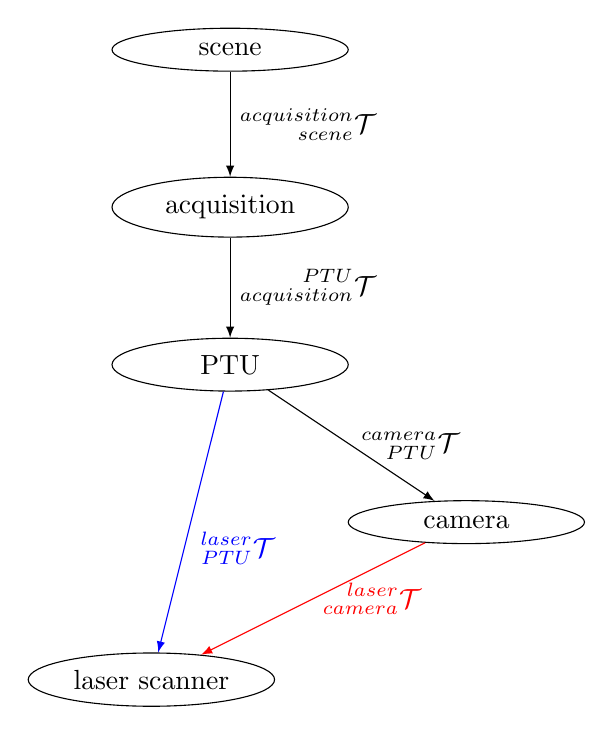
\begin{tikzpicture}
        % \node[draw, ellipse] (scene) {$scene$};
        % \node[draw, ellipse, right of=scene, xshift=3cm] (acquisition) {$acquisition$};
        % \node[draw, ellipse, right of=acquisition, xshift=3cm] (ptu) {$PTU$};
        % \node[draw, ellipse, right of=ptu, xshift=2cm] (laser) {$laser$};
        
        % \draw[-latex] (scene) -- (acquisition)
        % node[midway, above] {$\TF{scene}{acq}$};
        % \draw[-latex] (acquisition) -- (ptu)
        % node[midway, above] {$\TF{acq}{ptu}$};
        % \draw[-latex] (ptu) -- (laser)
        % node[midway, above] {$\TF{ptu}{laser}$};

        \tikzset{
            frame/.style={draw, ellipse, minimum width=3cm},
        }

        \node[frame] (scene) at (0,0) {scene};
        \node[frame] (acquisition) at (0, -2) {acquisition};
        \node[frame] (ptu) at (0, -4) {PTU};
        \node[frame] (camera) at (3, -6) {camera};
        \node[frame] (laser) at (-1, -8) {laser scanner};

        \draw[-latex] (scene) -- (acquisition)
            node[midway, right] {$\TF{scene}{acquisition}$};
        \draw[-latex] (acquisition) -- (ptu)
            node[midway, right] {$\TF{acquisition}{PTU}$};
        \draw[-latex] (ptu) -- (camera)
            node[midway, right] {$\TF{PTU}{camera}$};
        \draw[-latex, blue] (ptu) -- (laser)
            node[midway, below right] {$\TF{PTU}{laser}$};
        \draw[-latex, red] (camera) -- (laser)
            node[midway, right] {$\TF{camera}{laser}$};
    \end{tikzpicture}
    
    \caption{Transformation graph.}
    \label{figure:geometric-transformation-graph}
\end{figure}

\begin{equation}\label{eqn:point-registration}
    p_{i,j} = 
    \left[
        \begin{array}{c}
            x_{i,j} \\ y_{i,j} \\ z_{i,j} \\ 1 \\
        \end{array}    
    \right]
    =
    \TF{acq}{ptu}
    \cdot \TF{ptu}{laser}
    \cdot
    \left[
        \begin{array}{c}
            r_i \cos(\theta_i) \\
            r_i \sin(\theta_i) \\
            0 \\
            1 \\
        \end{array}    
    \right]
\end{equation}

At this phase, each point has 2 indexes, one for the laser scan index $j=1\dots L$ and another for the range index $i=1\dots N$, relative to the each laser scan. Therefore, at this stage, each point can be indexed with a pair of $(i,j)$ indexes. This point clouds are called structured point clouds.

This reconstruction phase depends heavily on the transformation from the PTU to the laser scanner. This transformation is obtained by a calibration process and is commonly referred to as the extrinsic calibration of the laser scanner.

In conclusion, for each acquisition results a point cloud with $L \times N$ points, where $L$ are the number of laser scans and $N$ the number of range values in each laser scan. Each point can be indexed in a bidimensional space, which is useful for subsequent algorithms.

\section{Laser Extrinsic Calibration}
\label{section:laser-extrinsic-calibration}


\section{Normal Estimation}
\label{section:normal-estimation}

As part of the reconstruction work, it is common to create a mesh using the point cloud, through a process called triangulation. Despite that in this work, this was not performed, it can be done in posterior work. Surface normals are a important property of geometric surfaces and are a requirement for most triangulation algorithms. Also, normals are required for lightning calculation, which can improve the rendering of a point cloud model\footnote{See "Estimating Surface Normals in a PointCloud" in \url{http://pointclouds.org/documentation/tutorials/normal_estimation.php}.}. As an example, the Stanford Bunny model\footnote{From \url{https://www.cc.gatech.edu/~turk/bunny/bunny.html}.} rendered with and without lightning are show in \cref{figure:bunny-normals}. As can be seen, lightning can improve the perception of the geometry of the point cloud model.

Normal estimation is quite trivial for surfaces, but for point clouds the process is quite not as easy. Usually there are two ways to estimate the normals: either by meshing the surface first, and then calculate the normals for the mesh, or using the point cloud itself to infer the normals. However, most meshing algorithms already require the normals to achieve a good result, so the latter option is more effective.

\begin{figure}[h]
    
    \centering
    \begin{subfigure}{0.4\textwidth}
        \centering
        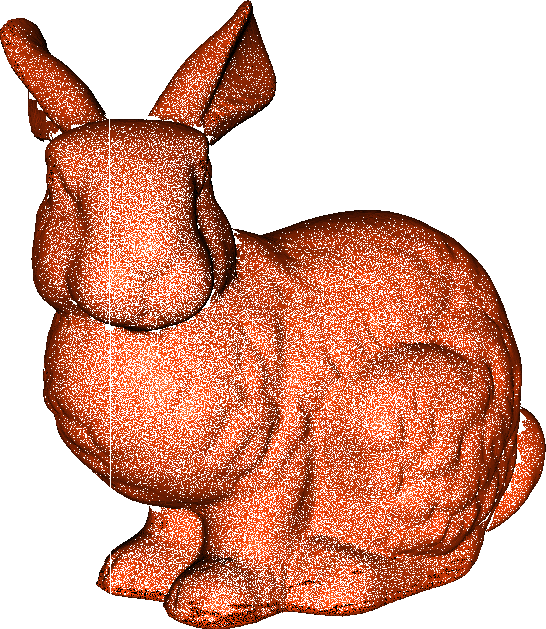
\includegraphics[height=6cm]{bunny-with-normals}     
    \end{subfigure}%
    \begin{subfigure}{0.4\textwidth}
        \centering
        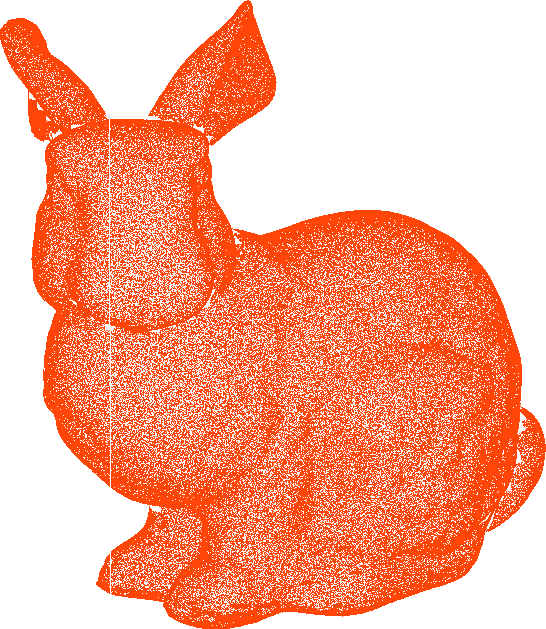
\includegraphics[height=6cm]{bunny-without-normals}     
    \end{subfigure}

    \caption{Stanford rabbit rendering with lightning (on the left), using the normals information, and without lightning (on the right).}
    \label{figure:bunny-normals}

\end{figure}

The most common solution is, for each point, to find the $k$ closest points, defined as the $k$-neighborhood of a point, and calculate the normal of the best-fitting plane formed by this points. However, finding the $k$-neighborhood of all the points in a point cloud has a time complexity $O(N \log N)$, so it can become quite slow for point clouds with a large number of points. In this work, an alternative solution was used to find the closest points, exploiting the bidimensional structure of the point cloud. This solution has a linear time complexity $O(N)$, which makes it a valuable solution for large point clouds.

The solution uses the fact that each point in the point cloud resulting from \cref{section:point-registration} has two indexes, one for the range index $i$ and one for the laser scan $j$. For each laser scan, each point $p_i$ has a neighborhood ${p_{i-k}, \ \dots, \ p_{i+k}}$, because each subsequent point has an increasing angle to the previous point. Between successive laser scans each point has an increasing angle (the pan angle) to the previous one. Therefore, for this algorithm, the neighborhood of each point: 

\begin{equation}
\label{eqn:point-neighborhood}
    neighborhood(p_{i,j}, k_1, k_2) = \{p_{i-k_1, j-k_2}, \ \dots, \ p_{i+k_1, j+k_2}\}.
\end{equation}

\noindent
The value of $k_1$ and $k_2$ have to be adjusted for a better result, because if the values are large, fine details are going to disappear and edges are going to be smeared, and on the other hand if the values are small, the surface will appear as too noisy. In this work, the value of $k_1$ and $k_2$ was 3, so the neighbor has 9 points.

Then, for each point, the tangent plane that fits the neighborhood is calculated, which in turn is a least-square plane fitting problem. This is usually solved by an analysis of Principal Component Analysis, as explained in \cref{section:calibration-cost-function}. This method will compute the direction of the normal $n$ for each point.

Then, the orientation of the point has to be defined, because the result of the PCA is ambiguous, which may lead to inconsistent normals in the point cloud. In this case, the solution found was to orientate the normals towards the frame of the 3D scanner, which for each acquisition in the origin of the coordinate system. Therefore, each normal has to satisfy:

\begin{equation}
\label{eqn:normal-orientation}
    n \cdot p < 0.
\end{equation}

\section{Acquisition Registration}
\label{section:acquisition-registration}

During an acquisition multiple acquisitions are done and to each one corresponds a transformation (position and orientation) to the scene referencial. In this section, a method is described to find each one of this transformations, so all the acquisitions are merged into a single point cloud. The method chosen is the ICP or Iterative Closest Point. This method is capable of aligning two point clouds, the reference and the target point cloud, by finding the transformation between the second to the first one. This is also known as point cloud registration.

\subsection{ICP}

This method can formally be described as follows: let $P$ be the target point cloud and $Q$ the reference point cloud. Then, the aim of the registration is to estimate the transformation $T$ from the referencial of $P$ to $Q$ by minimizing the error function $error(P, Q)$ in \cref{eqn:icp-transformation-function}, where $T(P)$ is the result of the application of the transformation $T$ to the point cloud $P$.

\begin{equation}
\label{eqn:icp-transformation-function}
    T = \underset{T}{argmin}(error(T(P), Q))
\end{equation}

The error function $error(P, Q)$ is computed on pair of points that are associated between the two point clouds. This association is, ideally, between points that are closest in position in both point clouds. Then, the distance between the matching points $(p_i, q_i)$ are used in the error function in \cref{eqn:icp-error-function}. The matching algorithm can be based on features or geometric properties, so a better matching can be found. In this work, a simple point-to-point matching.

\begin{equation}
\label{eqn:icp-error-function}
    error(P, Q) = \sum_{(p_i, q_i)}{|p_i - q_i|}
\end{equation}

In order to make the error function more robust, outlier points can be removed first from the match list. In addition, weights $w_i$ can be associated to each matching points $(p_i, q_i)$ to increase or decrease the influence of each matching points in the error function. As an example, normals can be used as a weight, so points with similar normals ($w_i = n_{p_i} \cdot n_{q_i}$) have a greater influence in the error function. 

However, the result of this minimization is always always dependant on the association between the points, which, unless the descriptors are good enough (like visual correspondences), the matching is not perfect, and is worst the farther apart both point clouds are. The idea behind the ICP algorithm is that, even with a bag association, the resulting estimate can be used to find a better one. So, the ICP algorithm creates a series of transformation $T_i$ at each iteration, yielding a new transformed point cloud $P_i$. Then, the next transformation is found:

\begin{equation}
    T_{i+1} = \underset{T}{argmin}(error(T_i(P_i), Q))
\end{equation}

Finally, the final transformation estimate is the composition of all the intermediary transformations:

\begin{equation}
    T = T_1 \circ T_2 \circ \dots \circ T_N
\end{equation}

\subsection{Multiple Point Cloud ICP}
\label{section:multiple-pointcloud-icp}

However, ICP can only register pairs of point clouds, whereas this work requires a registration of $N$ point clouds, corresponding to $n$ acquisitions. So, a technique has to be found so that the ICP algorithm can be used with $n$ point clouds. Three of this such techniques are now describes, ordered by their complexity.

The first approach and the easier one to implement is to register each point clouds sequencially. In other words, this method registers the point cloud $P_i$ to the point cloud $P_{i-1}$ and the transformation $T_{i-1}^{i}$ is found. The final accumulated point cloud is assembled using the \cref{eqn:registration-simple-method-calculation}. This method is the one that requires less overall registration, but has the downside that the transformation errors increases for each successive point cloud. This approach is shown in \cref{figure:multiple-icp-method-1}.

\begin{equation}
\label{eqn:registration-simple-method-calculation}
    P = \bigcup{\left(T_1^2 \circ T_2^3 \circ \dots \circ T_{i-1}^i\right)(P_i)}
\end{equation}

The next approach is widely used in robotics for Simultaneous Location and Mapping (SLAM). This method holds an accumulated point cloud $A$ in memory, and each new incoming point cloud $P$ registers to the accumulated point cloud and afterwards it is merged into $A$, which is then used for the next iteration, as shown in \cref{figure:multiple-icp-method-2}. It has the advantage that each new registration is done against a wider point cloud and has a smaller influence than in the previous method. Also, at each iteration the current pose of the 3D scanner is obtained, which is used as an initial estimate for the next iteration. However, the accumulated point cloud grows at each iteration, so a down-sampling is done at each iteration to keep the number of points bounded. In conclusion, each iteration can be calculated as:

\begin{align}
    T_{i} = & ICP(A, P_{i}, T_0 = T_{i-1}) \\
    A_{i+1} = & A{i} \bigcup T_{i}(P_i)
\end{align}

The last approach is the most complex. The idea of this approach is to minimize the number of transformation combinations, to minimize the propagation of the error. In particular, the registrations for the $N$ points clouds are done pairwise and are merged together to create $N/2$ point clouds. Then, this process is done recursively until an unique point cloud is obtained. This way, the maximum number of transformation combinations are equal to the number of levels of the tree, which is $\log_2(N)$, instead of $N$ combinations in the first approach. This algorithm is formalized in \cref{eqn:registration-tree-method-1,eqn:registration-tree-method-2}, for a list of point clouds $S=\left\{P_1, P_2, \ \dots, \ P_n\right\}$. At each level $l$ a new list of point clouds $^{l}P$ and transformations $^{l}T$ are computed, as shown in \cref{figure:multiple-icp-method-3}.

\begin{align}
    ^{l}T = & \left\{ICP(^{l-1}P_1, ^{l-1}P_2), \ \dots, \ ICP(^{l-1}P_{n-1}, ^{l-1}P_{n}) \right\}
        \label{eqn:registration-tree-method-1} \\
    ^{l}P = & \left\{^{l-1}P_1 \bigcup{^{l}T_1(^{l-1}P_2}), \ \dots, \ ^{l-1}P_{n-1} \bigcup{^{l}T_{n/2}(^{l-1}P_n)}\right\}
        \label{eqn:registration-tree-method-2}
\end{align}

In conclusion, three methods are possible to extend the ICP algorithm to multiple point clouds. After all the registrations are performed, point cloud can be assembled from all the point clouds, to form a big point cloud of the final scene. There is, however, a limitation of all this methods, because all of them have the principle that every point cloud is close to the previous one, which can be false. In this work, this was ensured in the capture methodology. 

\begin{figure}
    \centering
    \begin{subfigure}[t]{0.3\textwidth}
        \centering
        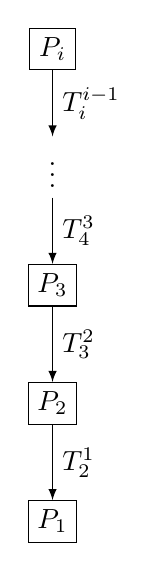
\begin{tikzpicture}
            \node[draw] (P1) at (0,0) {$P_1$};
            \node[draw] (P2) at (0,1.5) {$P_2$};
            \node[draw] (P3) at (0,3) {$P_3$};
            \node (P4) at (0,4.5) {$\vdots$};
            \node[draw] (Pi) at (0,6) {$P_i$};

            \draw[-latex] (P2) -- (P1) node[midway, anchor=west] {$T_2^1$};
            \draw[-latex] (P3) -- (P2) node[midway, anchor=west] {$T_3^2$};
            \draw[-latex] (P4) -- (P3) node[midway, anchor=west] {$T_4^3$};
            \draw[-latex] (Pi) -- (P4) node[midway, anchor=west] {$T_i^{i-1}$};
        \end{tikzpicture}

        \caption{First method}
        \label{figure:multiple-icp-method-1}
    \end{subfigure}%
    \begin{subfigure}[t]{0.3\textwidth}
        
        \centering
        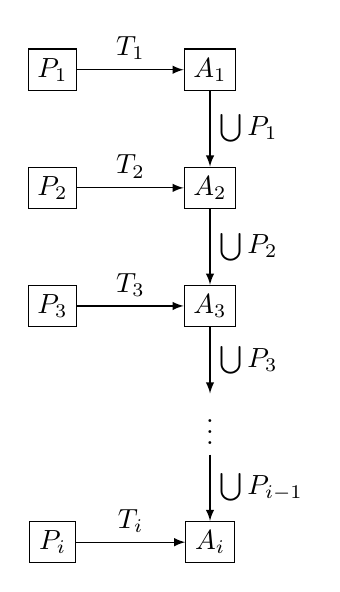
\begin{tikzpicture}
            \node[draw] (A1) at (0,0) {$A_1$};
            \node[draw] (A2) at (0,-1.5) {$A_2$};
            \node[draw] (A3) at (0,-3) {$A_3$};
            \node (A4) at (0,-4.5) {$\vdots$};
            \node[draw] (Ai) at (0,-6) {$A_i$};

            \node[draw, left of=A1, xshift=-1cm] (P1) {$P_1$};
            \draw[-latex] (P1) -- (A1) node[midway, above] {$T_1$};

            \node[draw, left of=A2, xshift=-1cm] (P2) {$P_2$};
            \draw[-latex] (P2) -- (A2) node[midway, above] {$T_2$};

            \node[draw, left of=A3, xshift=-1cm] (P3) {$P_3$};
            \draw[-latex] (P3) -- (A3) node[midway, above] {$T_3$};

            \node[draw, left of=Ai, xshift=-1cm] (Pi) {$P_i$};
            \draw[-latex] (Pi) -- (Ai) node[midway, above] {$T_i$};

            \draw[-latex] (A1) -- (A2) node[midway, right] {$\bigcup{P_1}$};
            \draw[-latex] (A2) -- (A3) node[midway, right] {$\bigcup{P_2}$};
            \draw[-latex] (A3) -- (A4) node[midway, right] {$\bigcup{P_3}$};
            \draw[-latex] (A4) -- (Ai) node[midway, right] {$\bigcup{P_{i-1}}$};
        \end{tikzpicture}

        \caption{Second method}
        \label{figure:multiple-icp-method-2}
    \end{subfigure}%
    \begin{subfigure}[t]{0.4\textwidth}
        
        \centering
        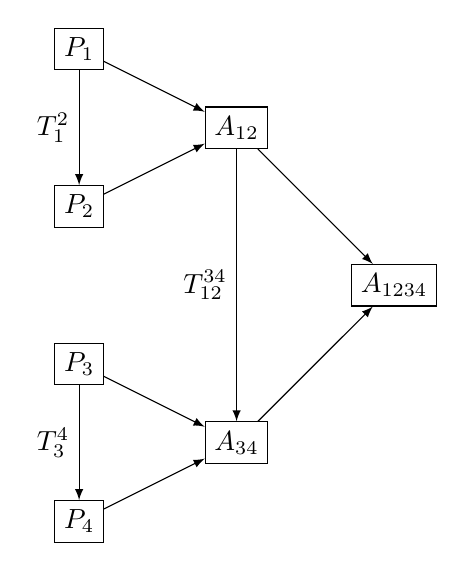
\begin{tikzpicture}
            \node[draw] (P1) at (0,0) {$P_1$};
            \node[draw] (P2) at (0,-2) {$P_2$};
            \node[draw] (P3) at (0,-4) {$P_3$};
            \node[draw] (P4) at (0,-6) {$P_4$};

            \node[draw] (A12) at (2, -1) {$A_{12}$};
            \node[draw] (A34) at (2, -5) {$A_{34}$};
            \node[draw] (A1234) at (4, -3) {$A_{1234}$};

            \draw[-latex] (P1) -- (A12);
            \draw[-latex] (P2) -- (A12);
            \draw[-latex] (P3) -- (A34);
            \draw[-latex] (P4) -- (A34);
            \draw[-latex] (A12) -- (A1234);
            \draw[-latex] (A34) -- (A1234);

            \draw[-latex] (P1) -- (P2) node[midway, left] {$T_1^2$};
            \draw[-latex] (P3) -- (P4) node[midway, left] {$T_3^4$};
            \draw[-latex] (A12) -- (A34) node[midway, left] {$T_{12}^{34}$};

        \end{tikzpicture}
        \caption{Third method}
        \label{figure:multiple-icp-method-3}
    \end{subfigure}%


    \caption{Multiple Point Cloud ICP approaches}
    \label{figure:registration-methods-approaches}
\end{figure}
\section{Filters}
\label{section:filters}

The final point cloud, after the assembly from every acquisition's point cloud, can have unnecessary or redundant information, which can make the point cloud size too large for any use. A common solution is to use filters to remote unnecessary points and downsample the point cloud.

\subsection{NaN Removal}

The first filter is the Not a Number removal, or NaN removal. In the first steps of the reconstruction, the point cloud is stored as a dense point cloud, or structured point cloud. To maintain this structure, NaNs are used to mark the missing values, which are usually originated by measurement errors. When the structure of the point cloud becomes irrelevant, its dimensions are collapsed into one. After, the NaNs become irrelevant and are removed from the point cloud.



In the acquisition, any range that is not measured is stored as a NaN, to signal that they are missing. During the point registration phase, all this missing ranges remain as NaN, and should be removed, because their information is irrelevant and take as much space as a real value. So, each point that contains a NaN value is removed from the final point cloud.

\subsection{Statistic Outlier Removal}

Usually point clouds contains different point densities, dependent on the distance of the object to the sensor. Also, measurement errors also occur next to edges or corners. As a result, point clouds tend to have sparse outliers that can affect subsequent algorithms, like segmentation or registration algorithms. A usual solution is to perform an statistically analysis on each point, removing the ones that do not reach a certain criteria. In particular, the mean distance of each point to its neighbors is computed, and if this distance is outside an interval centered in the mean of all the distances, then it is removed. An example can be seen in \cref{figure:sor-filter}.

\begin{figure}[h]
    
    \centering
    \begin{subfigure}[t]{0.5\textwidth}
        
        \centering
        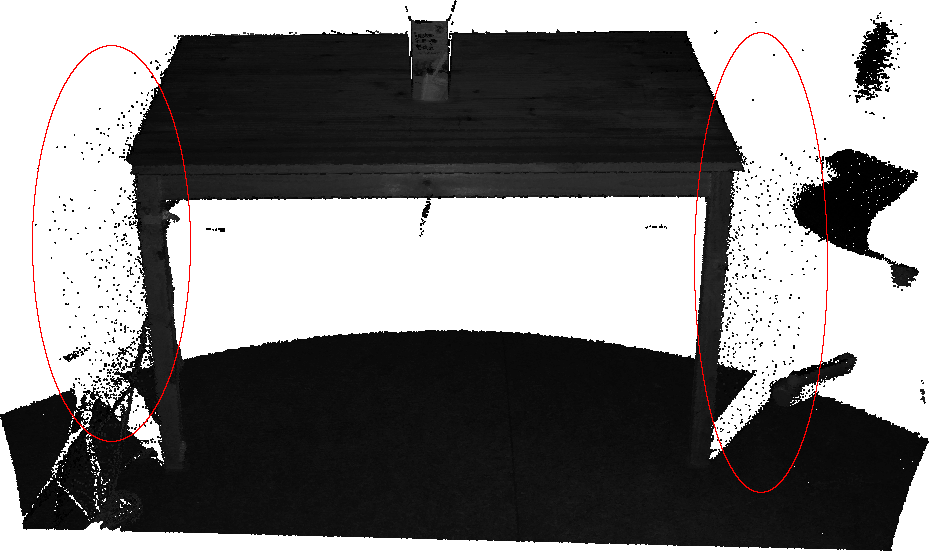
\includegraphics[width=0.8\textwidth]{table-with-outliers}
        \caption{Before SOR}
        \label{figure:sor-filter-before}
    \end{subfigure}%
    \begin{subfigure}[t]{0.5\textwidth}
        \centering
        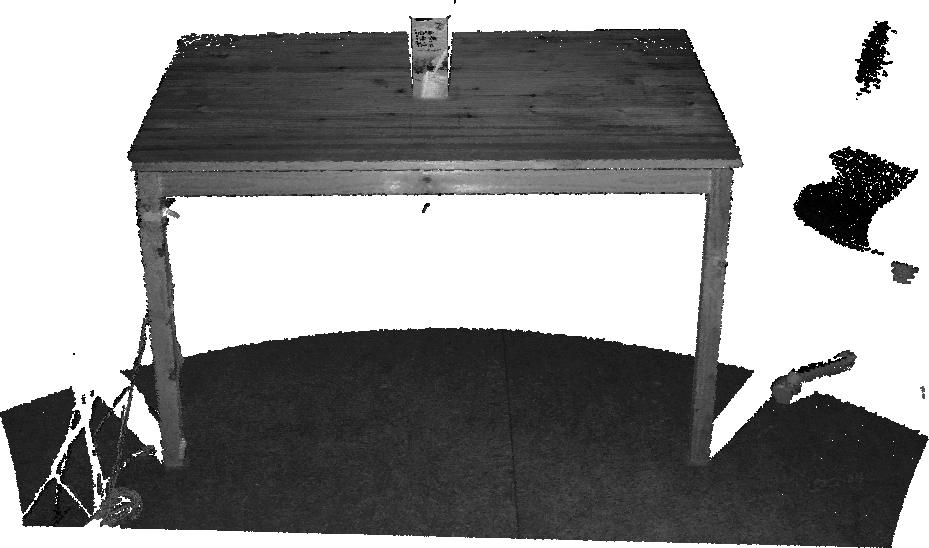
\includegraphics[width=0.8\textwidth]{table-without-outliers}
        \caption{After SOR}
        \label{figure:sor-filter-after}
    \end{subfigure}

    \caption{SOR filter in a point cloud, processed by the software \textit{CloudCompare}.}
    \label{figure:sor-filter}
\end{figure}

\subsection{Voxel Grid Downsampling}

This method downsamples, that is, reduce the number of points of a point cloud, using a voxel grid. A voxel is a cubical space and is the element in a tridimensional grid. So, each point in the point cloud belongs to some voxel. Then, in each voxel, all the points are represented by their centroid. This is an effective and fast method to downsample a point cloud. The level of detail can be parameterized with the voxel leaf-size (the size of each voxel in the $x,y,z$ direction). A smaller leaf-size maintains more details but generates a bigger point cloud. A bigger leaf-size does not keep as much detain but generates a smaller point cloud. As an example, \cref{figure:lucy-voxel-grid} shows the Stanford Lucy model\footnote{From "Stanford Scanning Repository" in \url{graphics.stanford.edu/data/3Dscanrep/}.} after a voxel grid downsampling with different leaf size values: \cref{figure:lucy-voxel-grid-2mm} with \SI{2}{\milli\meter} (288.000~pts), \cref{figure:lucy-voxel-grid-5mm} with \SI{5}{\milli\meter} (55.000~pts) and \cref{figure:lucy-voxel-grid-8mm} with \SI{2}{\milli\meter} (18.000~pts).

\begin{figure}[h]
    
    \centering
    \begin{subfigure}[t]{0.3\textwidth}
        \centering
        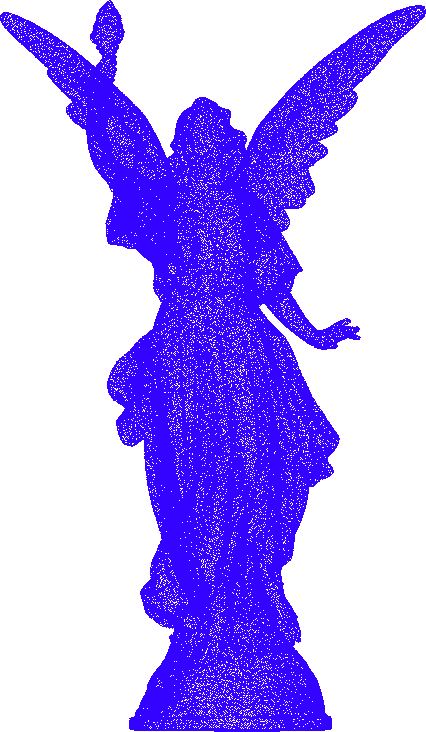
\includegraphics[height=6cm]{lady-voxel-2mm}
        \caption{Leaf size of \SI{2}{\milli\meter}}
        \label{figure:lucy-voxel-grid-2mm}
    \end{subfigure}%
    \begin{subfigure}[t]{0.3\textwidth}
        \centering
        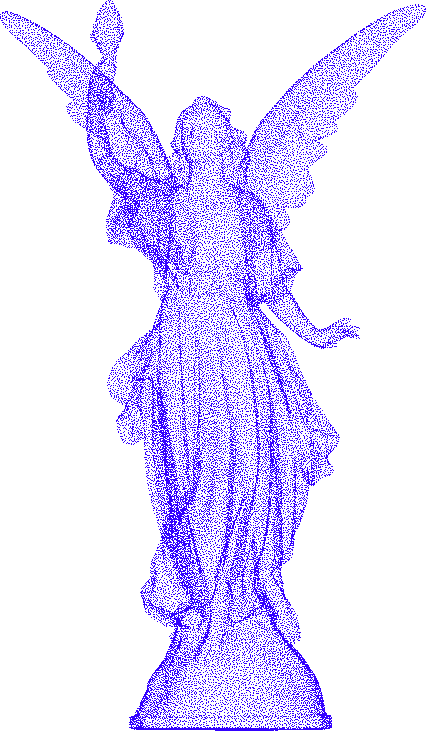
\includegraphics[height=6cm]{lady-voxel-5mm}
        \caption{Leaf size of \SI{5}{\milli\meter}}
        \label{figure:lucy-voxel-grid-5mm}
    \end{subfigure}%
    \begin{subfigure}[t]{0.3\textwidth}
        \centering
        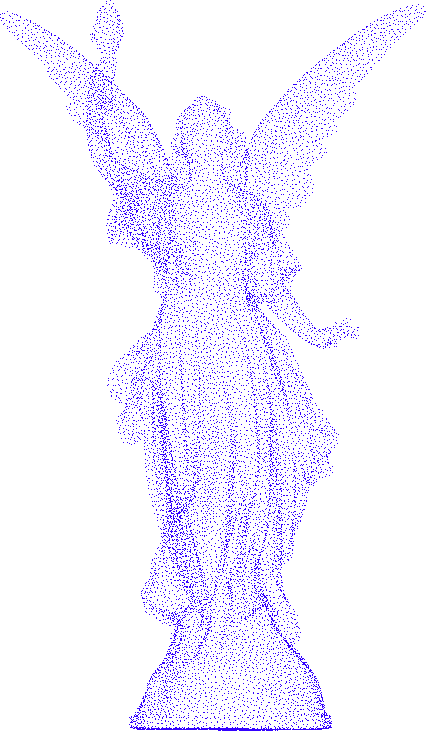
\includegraphics[height=6cm]{lady-voxel-8mm}
        \caption{Leaf size of \SI{8}{\milli\meter}}
        \label{figure:lucy-voxel-grid-8mm}
    \end{subfigure}

    \caption{Stanford Lucy scan after a voxel grid downsampling with different leaf sizes.}
    \label{figure:lucy-voxel-grid}
\end{figure}

\chapter{Methodology for Image Registration}
\label{section:methodology-for-image-registration}

\section{Pixel Registration}
\label{section:pixel-registration}

\subsection{Point Projection}
\label{section:point-projection}

\subsection{Occluded Point Rejection}
\label{section:occluded-point-rejection}

\subsection{Color Attribution}
\label{section:color-attribution}

\subsection{Color Fusion}

\section{Camera Intrinsic Calibration}
\label{section:camera-intrinsic-calibration}

\section{Camera Extrinsic Calibration}
\label{section:camera-extrinsic-calibration}
   

\chapter{Results}
\label{section:results}

In order to evaluate the proposed methods, multiple captures were taken from the department of Mechanical Engineering at the \textit{Universidade de Aveiro}. These proposed methods were tested with these captures and the results are shown in this chapter.

\section{Dataset Description}
\label{section:results-dataset-description}

In total, six captures were taken from three hallways of the department, using all the three lasers installed in the 3D scanner, one at each time. The hallways were chosen because of their large area and structured environment, with big and flat surfaces, making it easier to inspect the geometric quality of the scans. Also, small objects, like chairs, tables and doors can be found, as well as unstructured objects, like trees, can be found, which can be required to evaluate the color registrations. All the six captures can be found in \cref{table:captures}.

\begin{table}[h]
    \caption{Captures obtained to test the proposed methods.}
    
    \begin{tabu}{@{} X[1] X[3] X[2] X[2] @{}}
        \toprule
        & Scene   & Laser     & \#Acquisitions \\
        \toprule
        1 & Second Floor Hallway & Sick LMS100 & 7 \\
        \midrule
        2 & Third Floor East Hallway & Sick LMS100 & 12 \\
        \midrule
        3 & Third Floor East Hallway & Hokuyo URG04 & 9 \\
        \midrule
        4 & Third Floor West Hallway & Hokuyo URG04 & 10 \\
        \midrule
        5 & Second Floor Hallway & Hokuyo UTM30 & 6 \\
        \midrule
        6 & Third Floor East Hallway & Hokuyo UTM30 & 5 \\
        \bottomrule
    \end{tabu}

    \label{table:captures}
\end{table}


\section{Geometric Reconstruction}

The geometric reconstruction is the first part of the 3D reconstruction and uses the laser scanner data and the PTU transformation to obtain the non-colorized point cloud. This reconstruction relies on the extrinsic calibration of the laser to register the laser scans precisely, which is described in detain in \cref{section:laser-extrinsic-calibration}. Moreover, a new method to obtain the normals of the points was developed (\cref{section:normal-estimation}), as well as the methodology to register spatially the multiple acquisitions (\cref{section:acquisition-registration}). At the end of this registration, a point cloud resulted from all the acquisitions should be obtained.

\subsection{Extrinsic Laser Calibration}

The extrinsic calibration of the laser scanner is one of the prime factors of the geometric registration, because a bad calibration results in a deformed point cloud, as seen in \cref{figure:uncallibrated-pointcloud}. In this work, two calibration methods were used: one pre-existing method called RADLOCC and one method developed in this work, which attempts to be more accurate than the previous method. 

\begin{figure}[h]
    
    \centering
    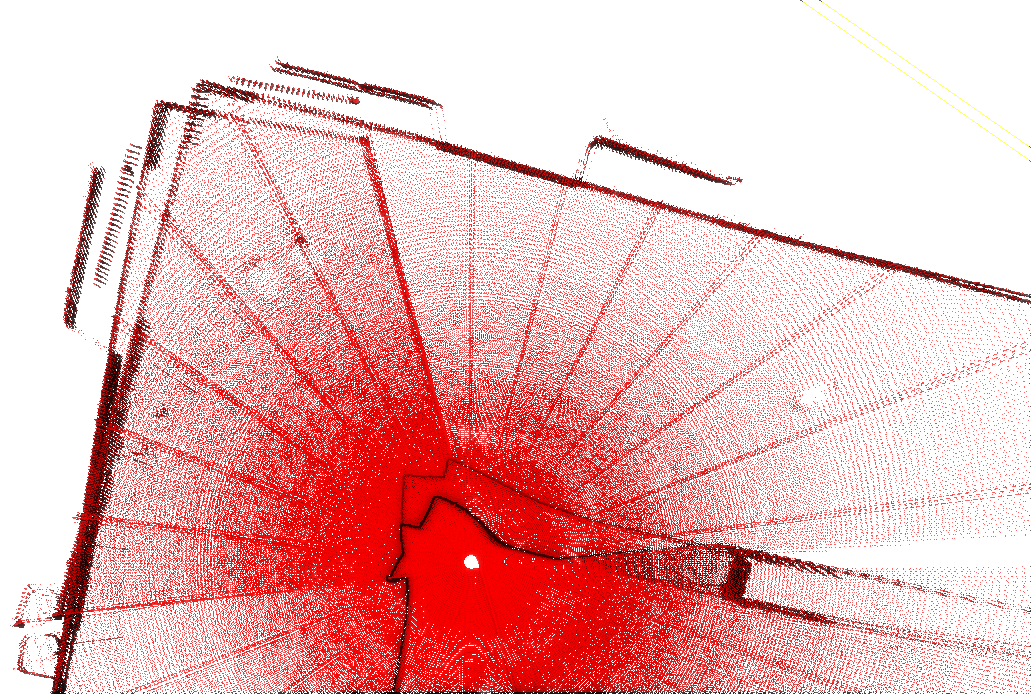
\includegraphics[width=0.7\textwidth]{uncallibrated-pointcloud}

    \caption{Uncalibrated point cloud of the capture 3}
    \label{figure:uncallibrated-pointcloud}

\end{figure}

\subsubsection{RADLOCC}

The RADLOCC calibration, described in \cref{section:radlocc-method}, was the first method used to obtain the extrinsic calibration of the laser scanner. This method requires multiple pairs of images and laser scans captured from a chessboard target. Then, the chessboard is extracted from both sensors and the calibration expects to match the extracted features. The evaluation of the calibration can be done by the re-projection of the laser scans onto the images, where the edges of the laser scan should be coincident with the edges of the chessboard, as seen in \cref{figure:radlocc-reprojection}. In total, six calibration datasets were obtained using the SICK LMS100 sensor, which have around 20 to 40 images and laser scans pairs. The results obtained are shown in table \cref{table:radlocc-results}.

\begin{figure}[h]
    
    \centering
    \begin{subfigure}{0.3\textwidth}
        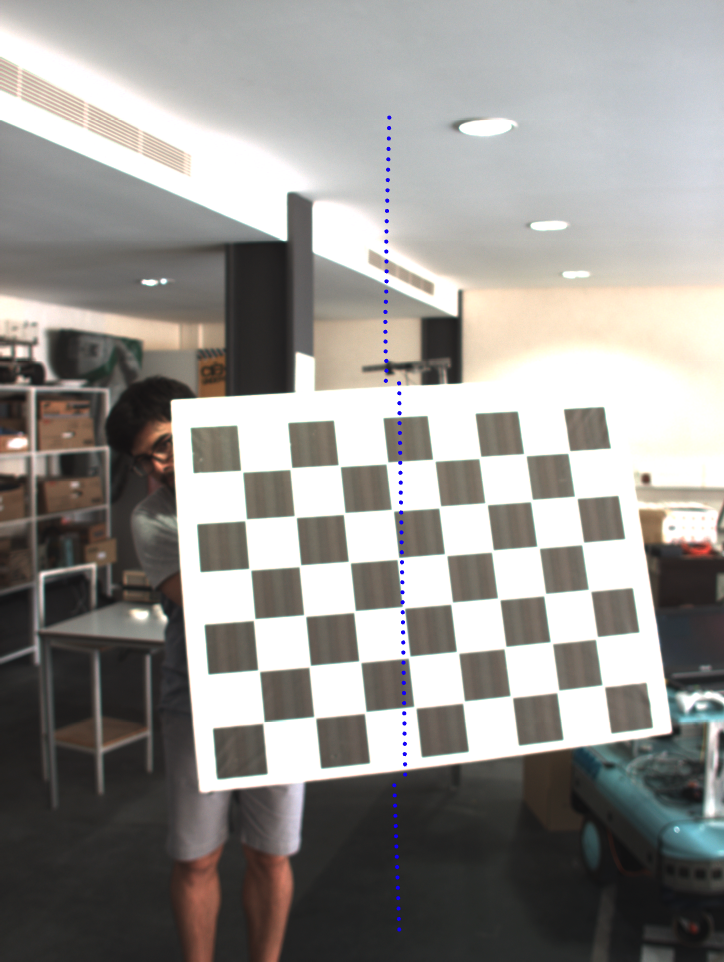
\includegraphics[height=6cm]{radlocc_calibration_1}
    \end{subfigure}%
    \begin{subfigure}{0.3\textwidth}
        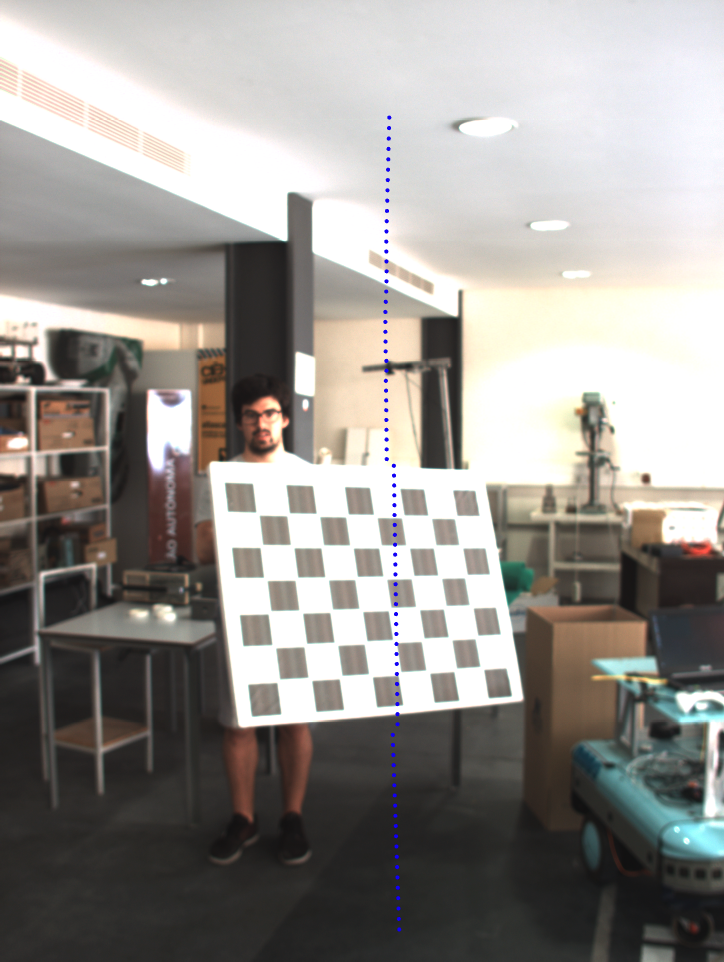
\includegraphics[height=6cm]{radlocc_calibration_2}
    \end{subfigure}%
    \begin{subfigure}{0.3\textwidth}
        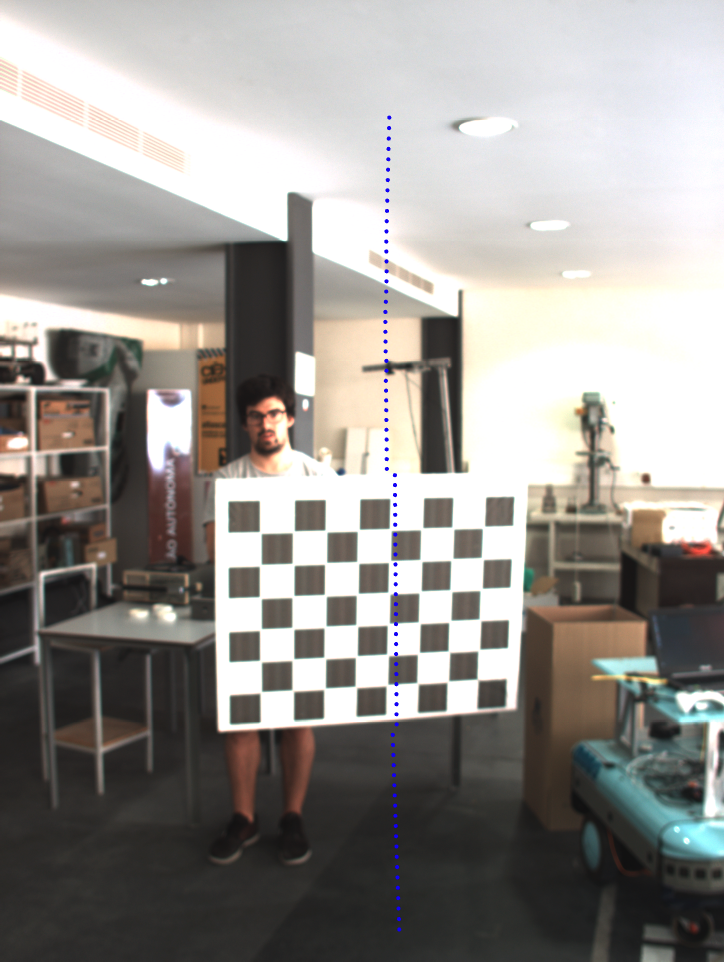
\includegraphics[height=6cm]{radlocc_calibration_3}
    \end{subfigure}%

    \caption{Reprojection of the laser scans in the images obtained in the RADLOCC calibration method.}

    \label{figure:radlocc-reprojection}

\end{figure}

\begin{table}[h]
    
    \caption{Resulting extrinsic calibration obtained using the RADLOCC method.}

    \centering
    \begin{tabu}{@{}c c ccc cccc@{}}
        \toprule
                &          & \multicolumn{3}{c}{translation} & \multicolumn{4}{c}{rotation} \\
                             \cmidrule(lr){3-5}\cmidrule(lr){6-9}
        Dataset & \#Images & $x$ & $y$ & $z$ & $x$ & $y$ & $z$ & $w$ \\
        \midrule
        1 & 28 & -0.0145 &  0.0435 & -0.0385 &  0.7129 & -0.0024 &  0.7008 & -0.0236 \\
        2 & 36 & -0.0242 &  0.0521 & -0.0926 &  0.7153 & -0.0082 &  0.6987 &  0.0059 \\
        3 & 38 &  0.0493 &  0.1823 & -0.0538 &  0.7113 &  0.0252 &  0.7005 &  0.0497 \\
        4 & 52 &  0.0190 &  0.0388 & -0.0561 &  0.7111 &  0.0005 &  0.7030 & -0.0077 \\
        5 & 15 & -0.0058 &  0.0850 & -0.0739 &  0.7183 &  0.0032 &  0.6956 & -0.0016 \\
        6 & 19 &  0.0072 & -0.0192 & -0.0334 &  0.7291 &  0.0247 &  0.6834 & -0.0245 \\
        7 & 14 &  0.0009 &  0.0699 & -0.0692 &  0.7126 &  0.0003 &  0.7013 & -0.0130 \\
        8 & 22 &  0.0212 &  0.0373 & -0.0641 &  0.7190 &  0.0074 &  0.6948 & -0.0131 \\
        \midrule
        $\mu$ \footnote{$\mu$ is the mean of the results.}
            &  &  0.0066 &  0.0612 & -0.0602 &  0.7162 &  0.0063 &  0.6973 & -0.0034 \\
        $\sigma$ \footnote{$\sigma$ is the standard variation of the results.}
            &  &  0.0217 &  0.0539 &  0.0180 &  0.0056 &  0.0115 &  0.0059 &  0.0223 \\
        \bottomrule
    \end{tabu}

    \label{table:radlocc-results}

\end{table}

As seen, the resulting transformations have a large deviation between calibration, both in rotation and translation. This, associated with the fact that the full extrinsic calibration requires the extrinsic calibration of the camera, which also has significant error, justifies that this method is not suitable or capable for this application. 

\subsubsection{Proposed method}

The proposed method for the calibration uses the same data as the one used for the geometric reconstruction. The first step is the segmentation of the planes by a manual approach using the software \textit{CloudCompare}. At the end of this step, each point has a correspondent integer index, which is called the cluster index. This method was required to be manual because the point cloud obtained by the initial estimate is deformed and the planes are not possible to be segmented by a automatic algorithm. In figure \cref{figure:segmented-pointcloud-full}, a segmented point cloud can be seen, correspondent to the capture 3. Specifically, the deformation of the point cloud results in planes that appear curved, discontinuous or duplicated, as seen in \cref{figure:segmented-pointcloud-detail}. It is expected that after the calibration this deformations are not existent.

\begin{figure}[h]
    
    \centering
    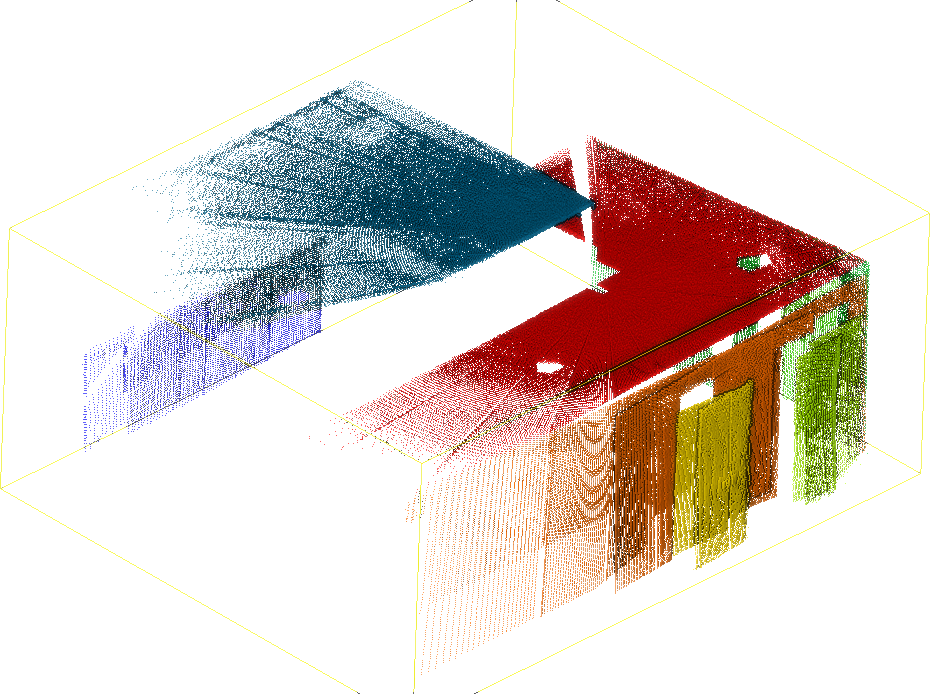
\includegraphics[width=0.8\textwidth]{segmented-pointcloud-full}
    \caption{Segmented point cloud from capture 3.}
    \label{figure:segmented-pointcloud-full}

\end{figure}

\begin{figure}[h]
    \centering
    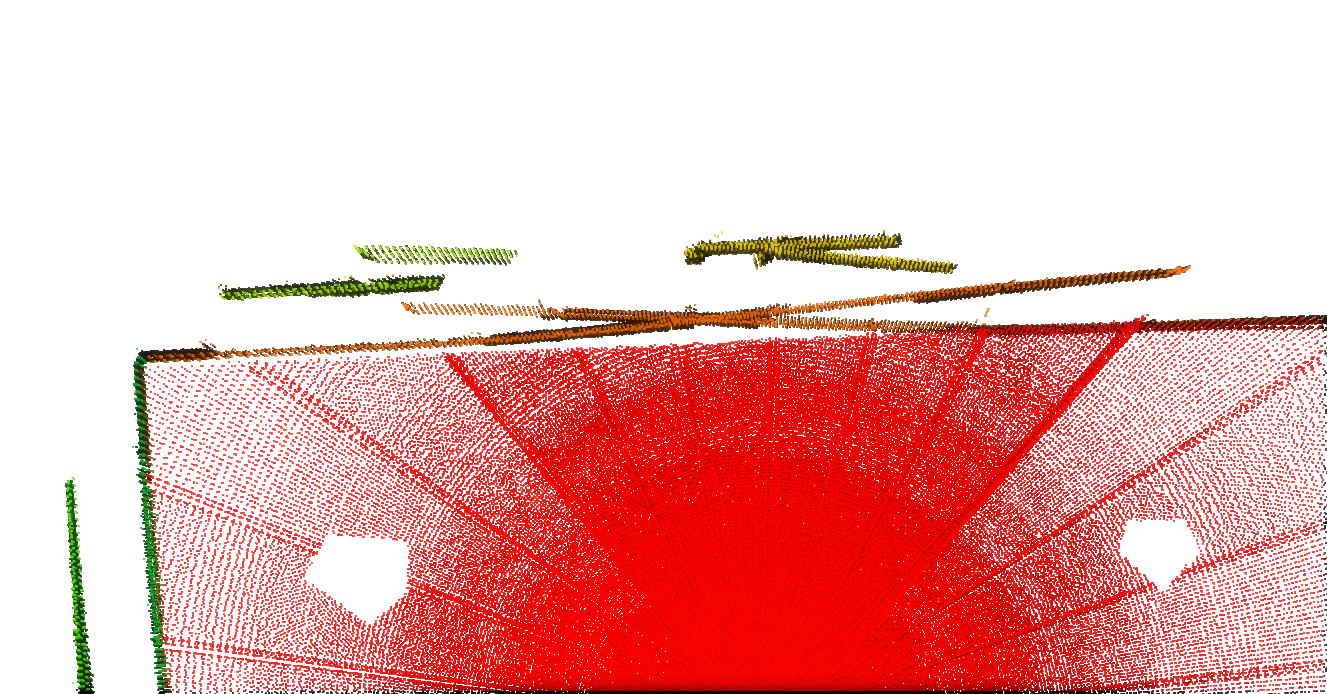
\includegraphics[width=0.8\textwidth]{segmented-pointcloud-detail}
    \caption{Detail of the segmented point cloud from capture 3.}
    \label{figure:segmented-pointcloud-detail}

\end{figure}

After the segmentation, the calibration score is minimized to obtain the extrinsic calibration of the laser scanner, as described in \cref{section:proposed-method}. For the initial estimate, a rough transformation was obtained via visual inspection. The result of a single acquisition is shown in \cref{figure:calibration-results-acquisition-3}. The initial score was \num{3.9e-3} and after 10 steps the score was reduced to about \num{1.1e-4}. The time required to this calibration is about \num{20}~minutes.

\begin{figure}[h]

    \centering
    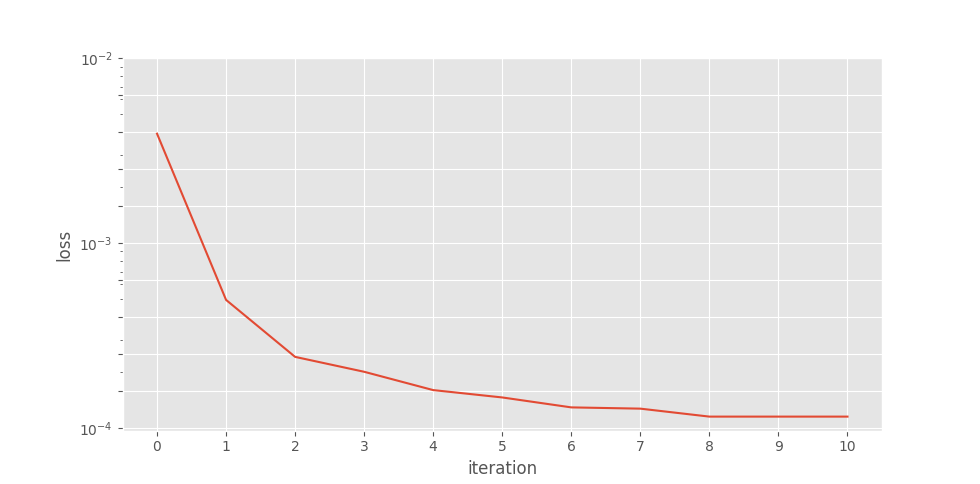
\includegraphics[width=0.7\textwidth]{calibration-iterations}
    
    \caption{Calibration iteration results for the third acquisition of the capture 4.}
    \label{figure:calibration-results-acquisition-3}
\end{figure}

The resulting calibration does indeed improve the geometry of the point cloud, shown before. In \cref{figure:calibration-comparison}, the resulting point cloud (in red) can be compared to the previous point cloud, obtained by the initial estimate. As can be seen, the deformation visible before are no longer present in the calibrated point cloud.

\begin{figure}[h]
    \centering
    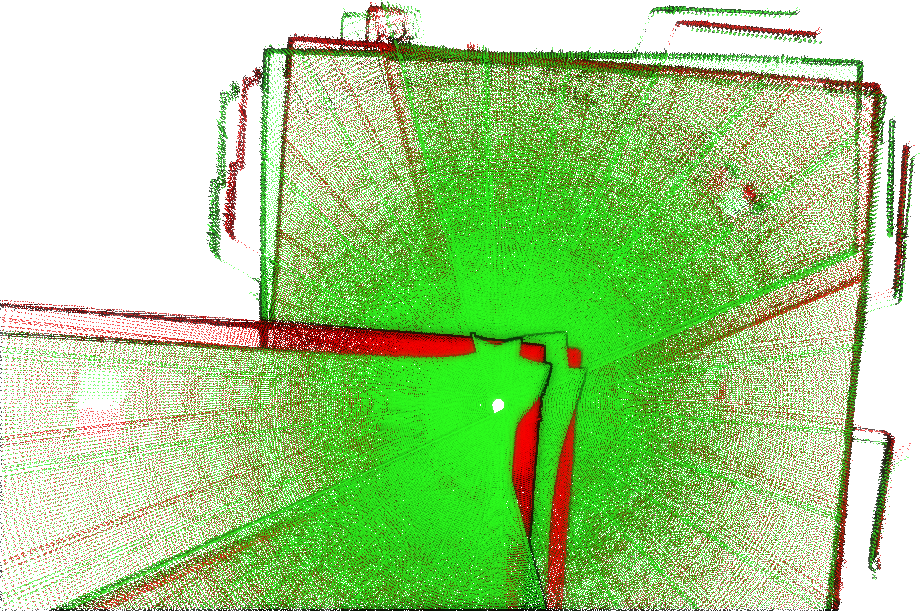
\includegraphics[width=\textwidth]{calibration-comparison}
    \caption{Comparison between the calibrated point cloud (in red) and the non-calibrated point cloud (in green)}
    \label{figure:calibration-comparison}
\end{figure}

In general, this calibration method successfully yields the same results for different acquisitions and captures. In other words, the calibration is repeatable. For example, the transformations obtained for a set of acquisitions of the capture 5 has similar results across the acquisitions, as shown in \cref{table:extrinsic-calibration-multiple-acquisitions}.

\begin{table}
    \caption{Extrinsic calibration obtained using multiple acquisitions}

    \centering
    \begin{tabu}{@{}c ccc c cccc@{}}
        \toprule
                    & \multicolumn{3}{c}{translation} & &  \multicolumn{4}{c}{rotation} \\
                             \cmidrule(lr){2-4}\cmidrule(lr){5-9}
        Acquisition & $x$ & $y$ & $z$ & & $q_x$ & $q_y$ & $q_z$ & $q_w$ \\
        \midrule
            1 & -0.00157 & 0.1195 & 0.1053 & & -0.5015 & -0.5151 & -0.5056 & 0.4770 \\
            2 &  0.00401 & 0.1103 & 0.0932 & & -0.5006 & -0.5175 & -0.5035 & 0.4776 \\
            3 &  0.00301 & 0.1222 & 0.0982 & & -0.5001 & -0.5168 & -0.5042 & 0.4782 \\
            4 &  0.00434 & 0.1321 & 0.0988 & & -0.5014 & -0.5158 & -0.5059 & 0.4761 \\
        \midrule
        $\mu$    & 0.00245 & 0.12103 & 0.09888 & & -0.50090 & -0.51630 & -0.50480 & 0.47723 \\
        $\sigma$ & 0.00237 & 0.00777 & 0.0043  & & 0.00058 & 0.00092 & 0.00099 & 0.00078 \\
        \bottomrule

    \end{tabu}

    \label{table:extrinsic-calibration-multiple-acquisitions}
\end{table}

Therefore, the proposed calibration can be a reliable method to obtain the extrinsic calibration of laser scanners mounted in motion platforms, as the PTU, because transformation obtained has the accuracy required for the geometric registration of the laser scanners for this work and the results have repeatability and reproductivity. The advantages of this method, compared to the previous method, are:

\begin{enumerate}
    \item The method directly obtains the extrinsic transformation of the laser scanner, instead of a partial transformation (to the camera). This also decreases the error that would come from the intrinsic and extrinsic calibration of the camera.
    \item This calibration uses exclusively the laser scanner data, which is more accurate than images. Moreover, the number of laser scans used are also greater than in the RADLOCC method, which can explain the lesser error found in this calibration method.
    \item This calibration acknowledges and benefits from the movement of the PTU, as opposed to the RADLOCC, which was designed for static laser scanners. The laser scanner has to be static in RADLOCC, so that the background segmentation of the laser scans is possible.
    \item The method proposed uses the data from the acquisitions directly, so the calibration process can be done even after the capture is made, or if the laser scanner is not available. This can be useful if the prior calibration did not have the accuracy required for the acquisition, for example, if the calibration was done using a smaller scene, or if the equipment has changed or is not available.
\end{enumerate}

\subsection{Normal Estimation}
\label{section:results-normal-estimation}

In this section, the results obtained from the Normal Estimation method described in \cref{section:normal-estimation} are shown and compared to the more traditional method using the $k$-nearest-Neighbors. Both methods have similar results, as shown in \cref{figure:normal-estimation-results}, however, there are differences:

\begin{enumerate}
    \item The proposed method relies on a continuous movement in pan, while recording the laser scans. However, this was not the case for the acquisitions, because the movement was interrupted to record the images. This explains the stripes of points with the wrong normals that are shown in the results.
    \item This method can only be used for each acquisition and can not be generalized for any point cloud, because it required that the point cloud is structured in a 2D structure. The other method, however, works for any point cloud.
    \item The computational complexity of the proposed method is $O(N)$, while the complexity of the method using the $k$-Neighbors is $O(N \log N)$, which has an increasing impact for large point clouds. For example, in a point cloud with 5 million points (for example, in captures 5 and 6), the time required to calculate the normals using the proposed method is \SI{10}{\second} (using a implementation in python, which is regarded as a slow language for numerical computations) and using the $k$-neighbors method the time required is about \SI{10}{\minute}.
\end{enumerate}

\begin{figure}[h]
    
    \centering
    \begin{subfigure}[t]{\textwidth}
        \centering
        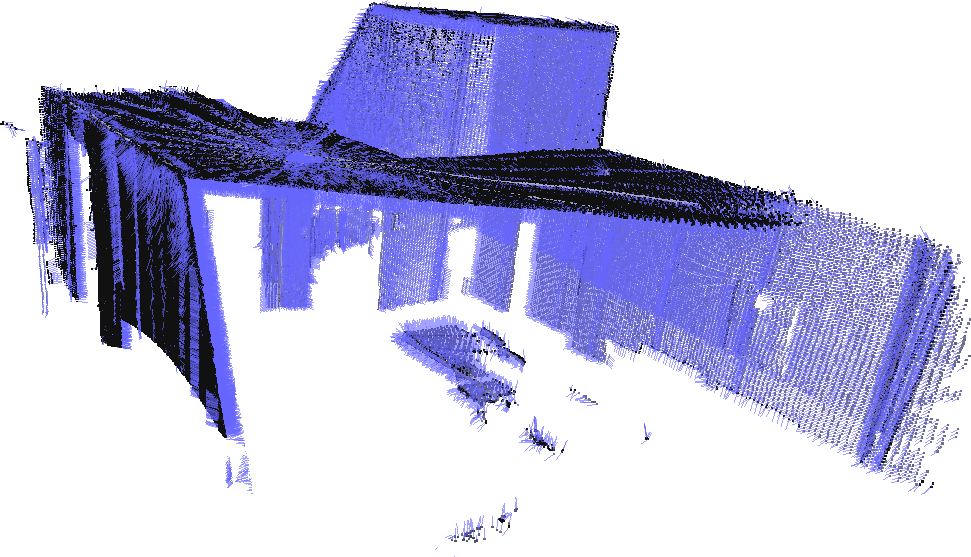
\includegraphics[width=0.7\textwidth]{normals-estimation-method}
        \caption{Normal estimation result using the proposed method.}
        \label{figure:normals-estimation-method}
    \end{subfigure}

    \begin{subfigure}[t]{\textwidth}
        \centering
        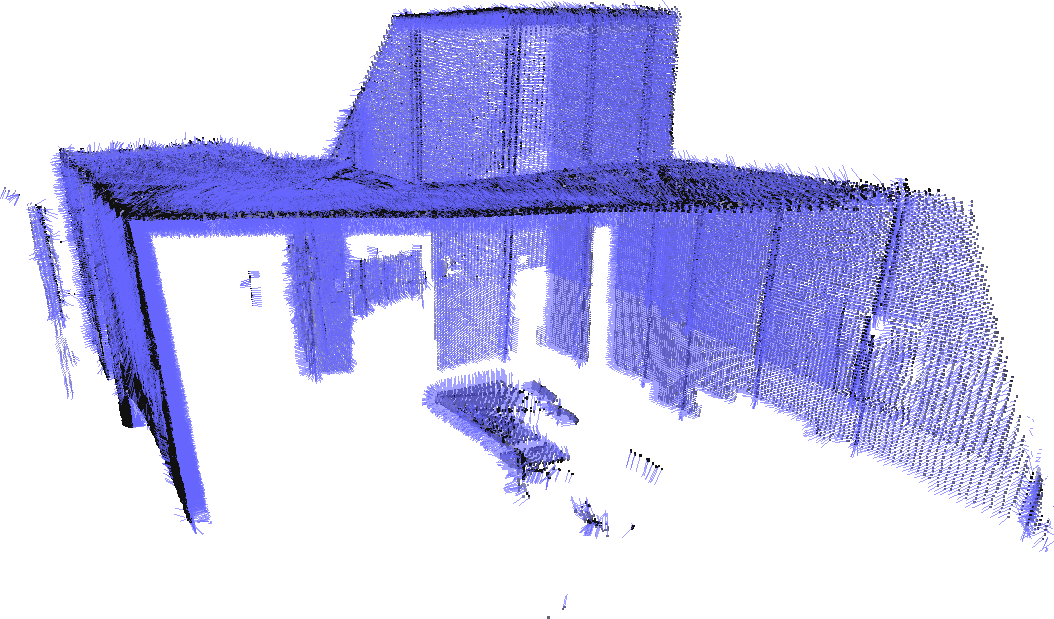
\includegraphics[width=0.7\textwidth]{normals-estimation-other-method}
        \caption{Normal estimation result using the common method.}
        \label{figure:normals-estimation-other-method}
    \end{subfigure}

    \caption{Comparison of both Normal estimation methods (the blue arrows represent the normal vector).}
    \label{figure:normal-estimation-results}

\end{figure}

\subsection{Acquisition Registration}

The method for the acquisition registration uses the ICP algorithm, which find the transformation between two point clouds by the minimization of the distance between the point clouds. This distance metric used was the distance between close points. However, finding the closest points in the two point clouds is a difficult task and can be wrong if two point clouds are far apart. In particular, the point clouds transformation is the distance between the acquisition poses, which is in the order of meters. The ICP method, however, is only successful for differences in the order of centimeters. Any difference greater than that results in a wrong registration, as seen in \cref{figure:icp-results}. The solution found was to manually align the point clouds first, and then use the ICP algorithm as a fine alignment. This solution is sub-optimal, as it is not automatic, thus requiring manual work. These shortcomings in the acquisition registration can be solved by either enhancing the ICP algorithm to improve the registration for large differences, or by providing the inicial estimate for the transformation between each acquisition.

\begin{figure}[h]
    
    \centering
    \begin{subfigure}[t]{0.5\textwidth}
        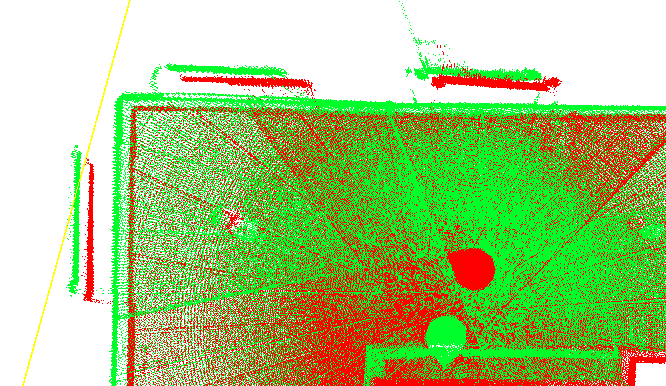
\includegraphics[width=\textwidth]{icp-registration-wrong-before}
        \caption{Before the ICP registration (incorrect).}
        \label{figure:icp-registration-wrong-before}
    \end{subfigure}%
    \begin{subfigure}[t]{0.5\textwidth}
        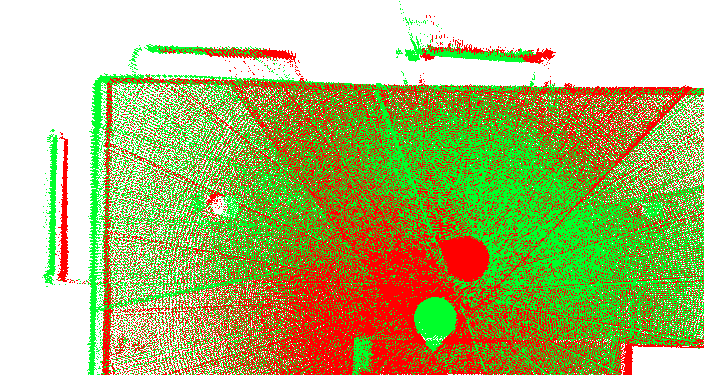
\includegraphics[width=\textwidth]{icp-registration-wrong-after}
        \caption{After the ICP registration (incorrect).}
        \label{figure:icp-registration-wrong-after}
    \end{subfigure}

    \begin{subfigure}[t]{0.5\textwidth}
        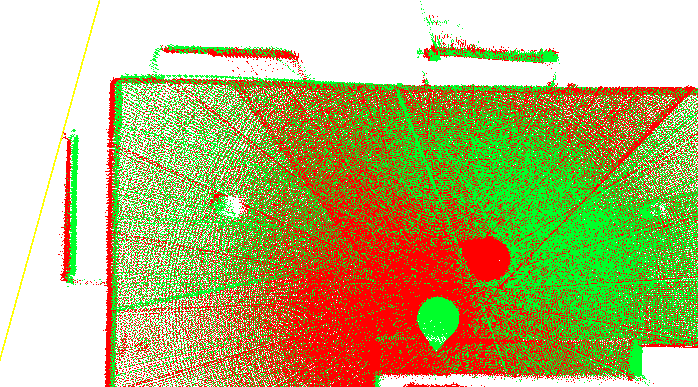
\includegraphics[width=\textwidth]{icp-registration-right-before}
        \caption{Before the ICP registration (correct).}
        \label{figure:icp-registration-right-before}
    \end{subfigure}%
    \begin{subfigure}[t]{0.5\textwidth}
        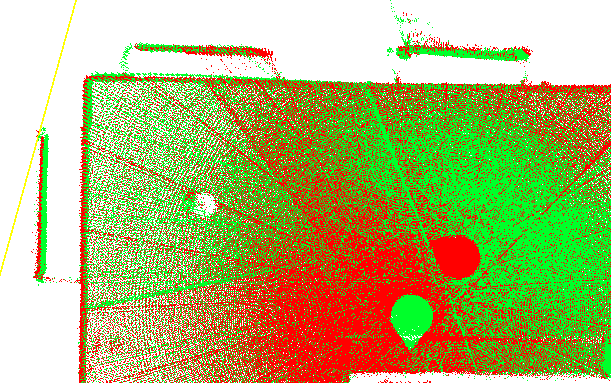
\includegraphics[width=\textwidth]{icp-registration-right-after}
        \caption{After the ICP registration (correct).}
        \label{figure:icp-registration-right-after}
    \end{subfigure}

    \caption{Comparison of the results regarding the ICP registration for different initial estimates. Two registration with a small difference result (\cref{figure:icp-registration-right-before,figure:icp-registration-wrong-before}) can yield two different outcomes (\cref{figure:icp-registration-right-after,figure:icp-registration-wrong-after}).}
    \label{figure:icp-results}

\end{figure}

Another disadvantage of the ICP algorithm is that the registration is pairwise. In this work, multiple point clouds were registered, and the inability of the ICP to register more than two point clouds at once implies that the registration does not use the full spectrum of data available, and is constrained to only the two point clouds at each registration. This suggests that a registration which is done between two point clouds with small overlap, which results in a weaker registration, could be avoided. If the algorithm used the entire data set, the registration would be done with the most overlap possible, and number of common points is maximized. To circumvent this problem, the three alternative methods are shown in \cref{section:acquisition-registration}. However, only the second method was proven to be effective in this work. This method registers the point clouds to an accumulated point cloud resulted by the fusion of the prior registered point clouds. The success of this method can be explained due to the increasing overlap existent in further registrations. In fact, the registrations that are done last are usually faster and more accurate (based on the output RMS value of the ICP algorithm).

In conclusion, the ICP algorithm is not sufficient for an automatic registration of the acquisitions. However, with manual intervention as a first registration, the ICP algorithm can be used to find the fine registration of the acquisitions. Using this method, the registrations were possible, as shown in \cref{figure:icp-results}.

\begin{figure}[h]
    
    \centering
    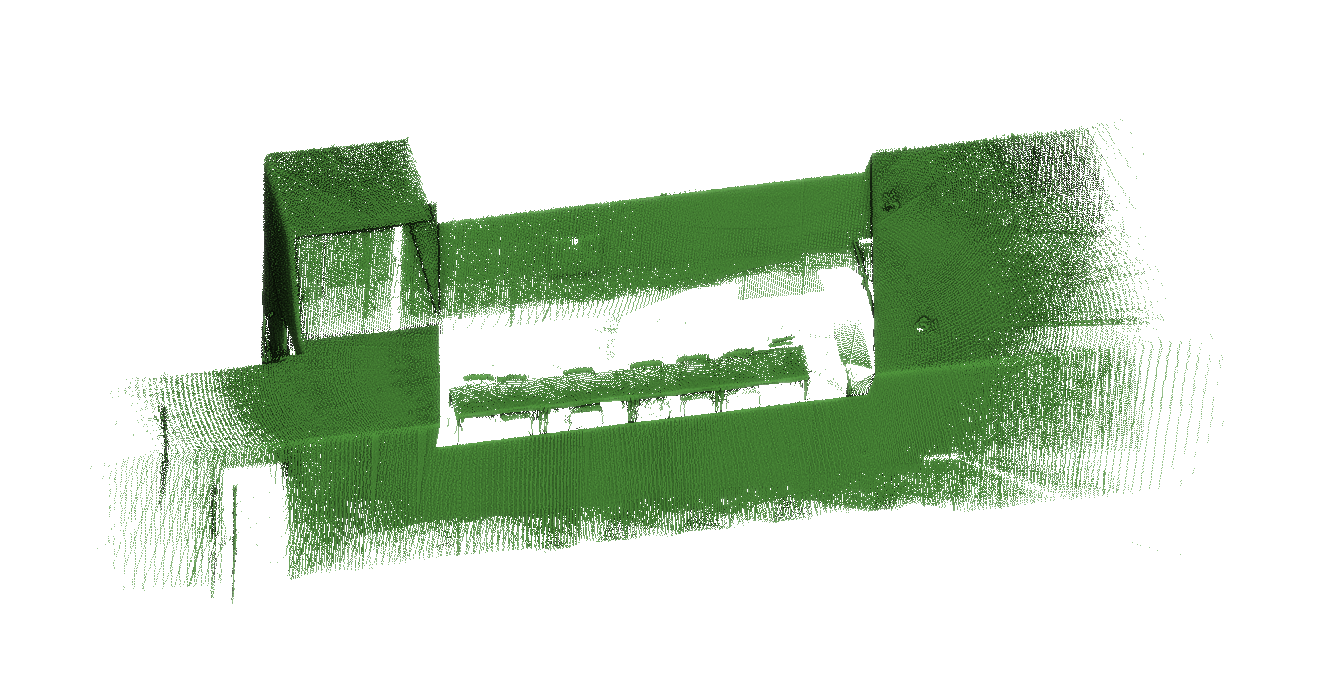
\includegraphics[width=\textwidth]{icp-result}

    \caption{Resulting fusion of all point clouds obtained in the capture 3, after the acquisition registration.}
    \label{section:icp-result}

\end{figure}

\subsection{Influence of the different laser scanners}

In this work, three different laser scanners were used to study the influence of the different characteristics of each one on the reconstruction process. 

Firstly, the aperture of the laser and the range are important factors in the capture process. As an example, the Hokuyo URG04 has a small range of \SI{5.6}{\meter}, compared to the larger range of the two other lasers, which both have a range of \SI{30}{\meter}. The resulting point clouds are, then, much smaller in the case of the Hokuyo~URG04, which means that more acquisitions are required to capture a scene, and the distance between each acquisition should not be larger that the range of the laser scanner. Otherwise, there is no overlap between acquisitions so the acquisition registration would fail. The same can be applied to the aperture of the laser scanner. 

Secondly, the response of the same surfaces differ from laser to laser, mostly due to the wavelength and energy of the laser used. As an example, the floor surface, which was made of tiles with reflective material, was only properly registered in the SICK LMS100 laser scanner, which is the laser with the most power output. It is expected to be due to the high reflection of the surface, so only a small fraction of the laser beams is reflected back to the laser scanner. If the laser emitted does not have considerable power, the reflected light could not have sufficient energy to be detected by the sensor. 

Thirdly, the statistical error of the measurements of the laser scanner can influence the quality of the point cloud. In other words, if the statistical error is large, the the points belonging to the same surface will be more scattered. This can have a large effect on the extrinsic calibration of the laser scanner, as it relies on the surface points to obtain the calibration.

Moreover, the scanning rate of the laser scanner can be important to obtain dense point clouds, without requiring a large acquisition time. The Hokuyo UTM30 was the laser scanner with the higher scanning rate (\SI{40}{\hertz}), which produced point clouds with about 4 times the number of points obtained by the two other lasers, without sacrificing the acquisition time.

Lastly, the SICK LMS100 laser was found to be unsuitable for this application, because the laser scans obtained were not accurate, compared to the other sensors. The laser scans of planar surfaces appear as deformed in this laser scanner. This can be seen in \cref{figure:deformed-laser}, where both the floor and the root are not shown as curved lines. Therefore, the resulting point clouds were always deformed, even after many extrinsic calibrations. The source of the problem was not identified, but is suspected to be due to a damaged laser scanner, or the laser scanner in question does not have the required accuracy for this application. Therefore, the acquisitions of this laser are not considered further on.

\begin{figure}[h]
    
    \centering
    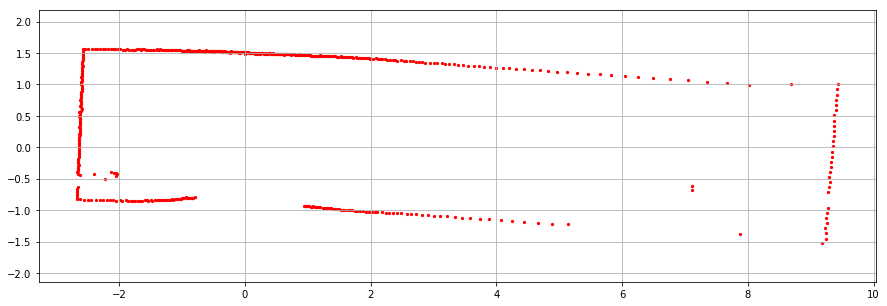
\includegraphics[width=\textwidth]{laser-deformation}

    \caption{Deformed laser of the LMS100 laser scanner.}
    \label{figure:deformed-laser}

\end{figure}

\subsection{Overall Results}

The results of the geometric registration are satisfactory, mostly because of the new calibration method of the laser, which ensured the success all the geometric algorithms used further on, such as the normal estimation and the acquisition registration. The overall results are shown in \cref{figure:results-capture-5,figure:results-capture-6}.


\begin{figure}[h]

    \centering
    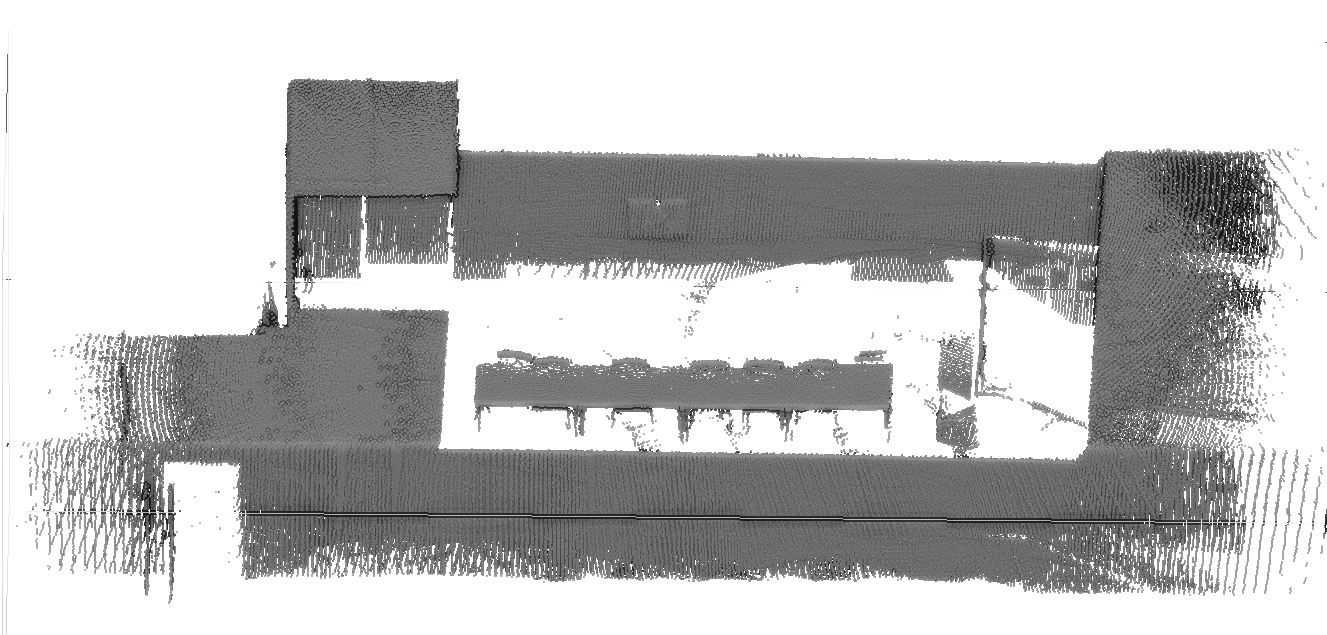
\includegraphics[width=\textwidth]{geometry-result-2}

    \caption{Result of the geometric reconstruction of the capture 5.}
    \label{figure:results-capture-5}
    
\end{figure}

\begin{figure}[h]

    \centering
    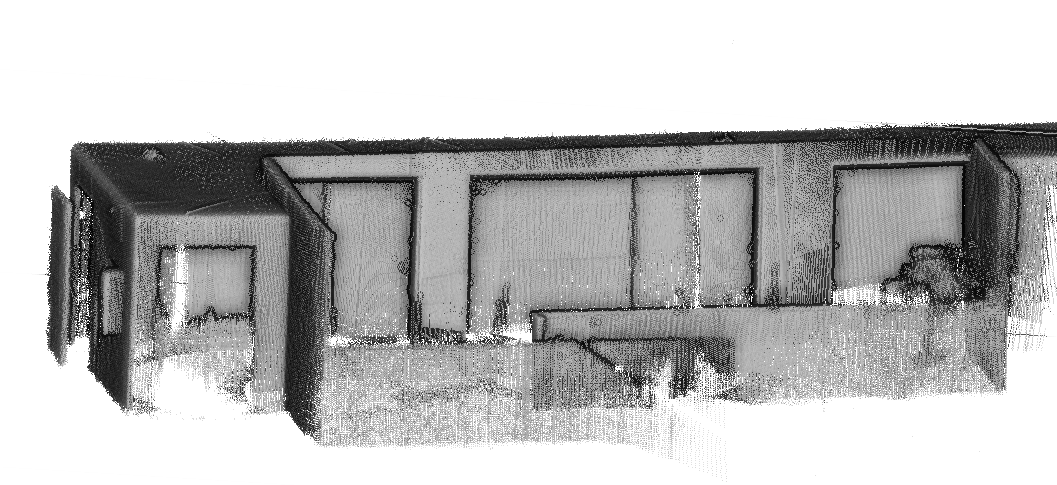
\includegraphics[width=\textwidth]{geometry-result-1}

    \caption{Result of the geometric reconstruction of the capture 6.}
    \label{figure:results-capture-6}
    
\end{figure}

\section{Color Reconstruction}

The color reconstruction is the final part of the reconstruction, which uses the images taken from the camera and registers the color into the point cloud obtained in the geometric reconstruction and merges the colors to obtain a colorized point cloud. This methods require both the intrinsic and extrinsic calibration of the camera, to register the images correctly. 

\subsection{Camera Intrinsic Calibration}

This calibration obtains the intrinsic parameters of the camera, as the focal length and center point. In total, three calibrations were done, which are shown in \cref{table:camera-intrinsic-calibration-results}. As can be seen, the results of the calibrations are similar between calibration. The calibration method used is widely used so it is expected that the results are accurate. 

\begin{table}[h]
    \caption{Results of the intrinsic calibration of the camera}

    \centering
    \begin{tabular}{@{} c cc c cc c cccc @{} }
        \toprule
           & \multicolumn{2}{c}{center point} & & \multicolumn{2}{c}{focal length} & & \multicolumn{4}{c}{distortion coefficients} \\
        \cmidrule{2-3} \cmidrule{5-6} \cmidrule{8-11}

        {calibration} & $x$ & $y$ &  & $x$ & $y$ & & $k_1$ & $k_2$ & $p_1$ & $p_2$  \\
        \midrule
        0 &   987.64 & 734.81 & & 2188.83 & 2184.15 & & -0.224 & 0.187 & 0.00110 & 0.000499  \\
        1 &  1008.60 & 724.81 & & 2181.50 & 2181.45 & & -0.214 & 0.182 & 0.00175 & 0.001327  \\
        2 &   985.64 & 755.84 & & 2147.93 & 2153.79 & & -0.211 & 0.195 & 0.00222 & 0.002553  \\
        \midrule
        $\mu$    & 994.0 & 738.5 & & 2173   & 2173   & & 0.216 & 0.188 & 0.00169  & 0.00146 \\
        $\sigma$ &  10.4 &  12.9 & &   17.8 &   13.7 & & 0.006 & 0.005 & 0.00046  & 0.00084 \\
        \bottomrule
    \end{tabular}

    \label{table:camera-intrinsic-calibration-results}
\end{table}

\subsection{Camera Extrinsic Calibration}

The method used to obtain the extrinsic calibration of the camera was the hand-in-eye calibration method. In this work, an ArUCO marker with a side of \SI{200}{\milli\meter} was placed about \SI{2}{\meter} away from the camera. The PTU was then manually controlled to capture different images of the marker in different poses of the camera. After about 30 poses, the calibration was done. The number of calibration done using this method were 3, and the results are shown in \cref{table:camera-extrinsic-calibration-results}. The results are very close between calibrations however, further on it can be seen that the results of this calibration is sub-optimal and is not sufficient for the registration of color for distances larger than \SI{2}{\meter}.

\begin{table}[h]
    \caption{Results of the extrinsic calibration of the camera.}

    \centering
    \begin{tabu}{@{}l ccc cccc @{}}
        \toprule
            &       \multicolumn{3}{c}{translation} & \multicolumn{4}{c}{rotation} \\
                             \cmidrule(lr){2-4}\cmidrule(lr){5-8}
        calibration &  $x$ &  $y$ &  $z$ &  $q_x$ &  $q_y$ &  $q_z$ & $q_w$ \\
        \midrule
        0 & -0.103524 &      -0.086451 &       0.050509 & 0.027264 &   -0.702682 &   -0.024205 &  0.710570 \\
        1 & -0.100458 &      -0.088829 &       0.049478 & 0.030372 &   -0.701046 &   -0.027414 &  0.711941 \\
        2 & -0.098975 &      -0.084319 &       0.046249 & 0.033105 &   -0.702234 &   -0.031446 &  0.710481 \\
        3 & -0.101184 &      -0.089208 &       0.052215 & 0.029564 &   -0.702891 &   -0.025002 &  0.710243 \\
        \midrule
        $\mu$
          & -0.10104  &      -0.087202 &       0.049613 & 0.030076 &   -0.702213 &   -0.027017 &  0.710808 \\
        $\sigma$
          & 0.001643  &       0.001971 &       0.002174 & 0.002088 &    0.000714 &    0.002817 &  0.000665 \\
        \bottomrule
        \end{tabu}


    \label{table:camera-extrinsic-calibration-results}
\end{table}

The failure of this calibration can be related to multiple shortcomings in this calibration method. First, this calibration uses an ArUCO as the marker for the pose estimation. It is possible that the error associated with the pose estimation can be large, jeopardizing the subsequent calibration. Second, the limited field of view of the camera limits the range of the movements of the PTU for a small interval of angles in pan and tilt. This limitation in space can result in a limited space of angles registered, which can therefore impact the accuracy of the result. Hence, this calibration fails to obtain an accurate extrinsic calibration of the camera.

\subsection{Color Registration and Fusion}

In the color registration and fusion process, the color is attributed to each point in the point cloud. In short, the color registration defines how each point is colorized, based on an image, and the fusion process defines what is the resulting color, after all the images are registered. In total, six methods were approached in this work for the color fusion: the first three methods choose a color from all the registered color and the last three methods calculate the average of all the colors, though a simple mean, or a weighted mean.

The registration process was, however, not perfect, mostly due to a imperfect calibration of the camera. Therefore, the color are not registered in their correct positions, as seen in \cref{figure:wrong-registration-photocopy}. In this image, the colors from different object are registered in wrong objects, for example, the elevator door. Also, the discontinuities are result of this inaccurate registration.

\begin{figure}[h]
    
    \centering
    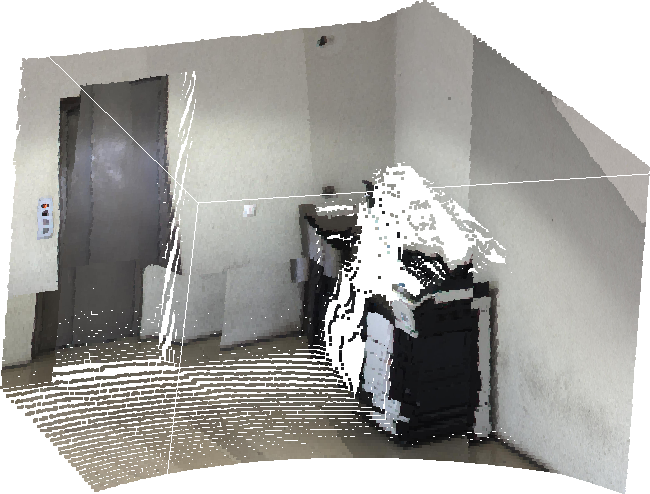
\includegraphics[width=0.6\textwidth]{color-registration-1}

    \caption{Example of the inaccurate color registration.}
    \label{figure:wrong-registration-photocopy}
\end{figure}

Also, the images taken have different color values for the same objects. This is due to illumination differences at the capture of each image. This difference is also noticed in the colorized point clouds. This problem is hard to solve, but can be mitigated by ensuring an uniformly illuminated scene. Even so, direct sunlight or shadows negatively affect the colorization. This problem can be shown is the images in \cref{figure:illumination-issues-images}, where the differences in color are very noticeable. The resulting colorization has, therefore, the same variation in color as the one present in the images, as shown in \cref{figure:illumination-issues-pointcloud}.

\begin{figure}[h]
    
    \centering
    \begin{subfigure}{0.5\textwidth}
        \centering
        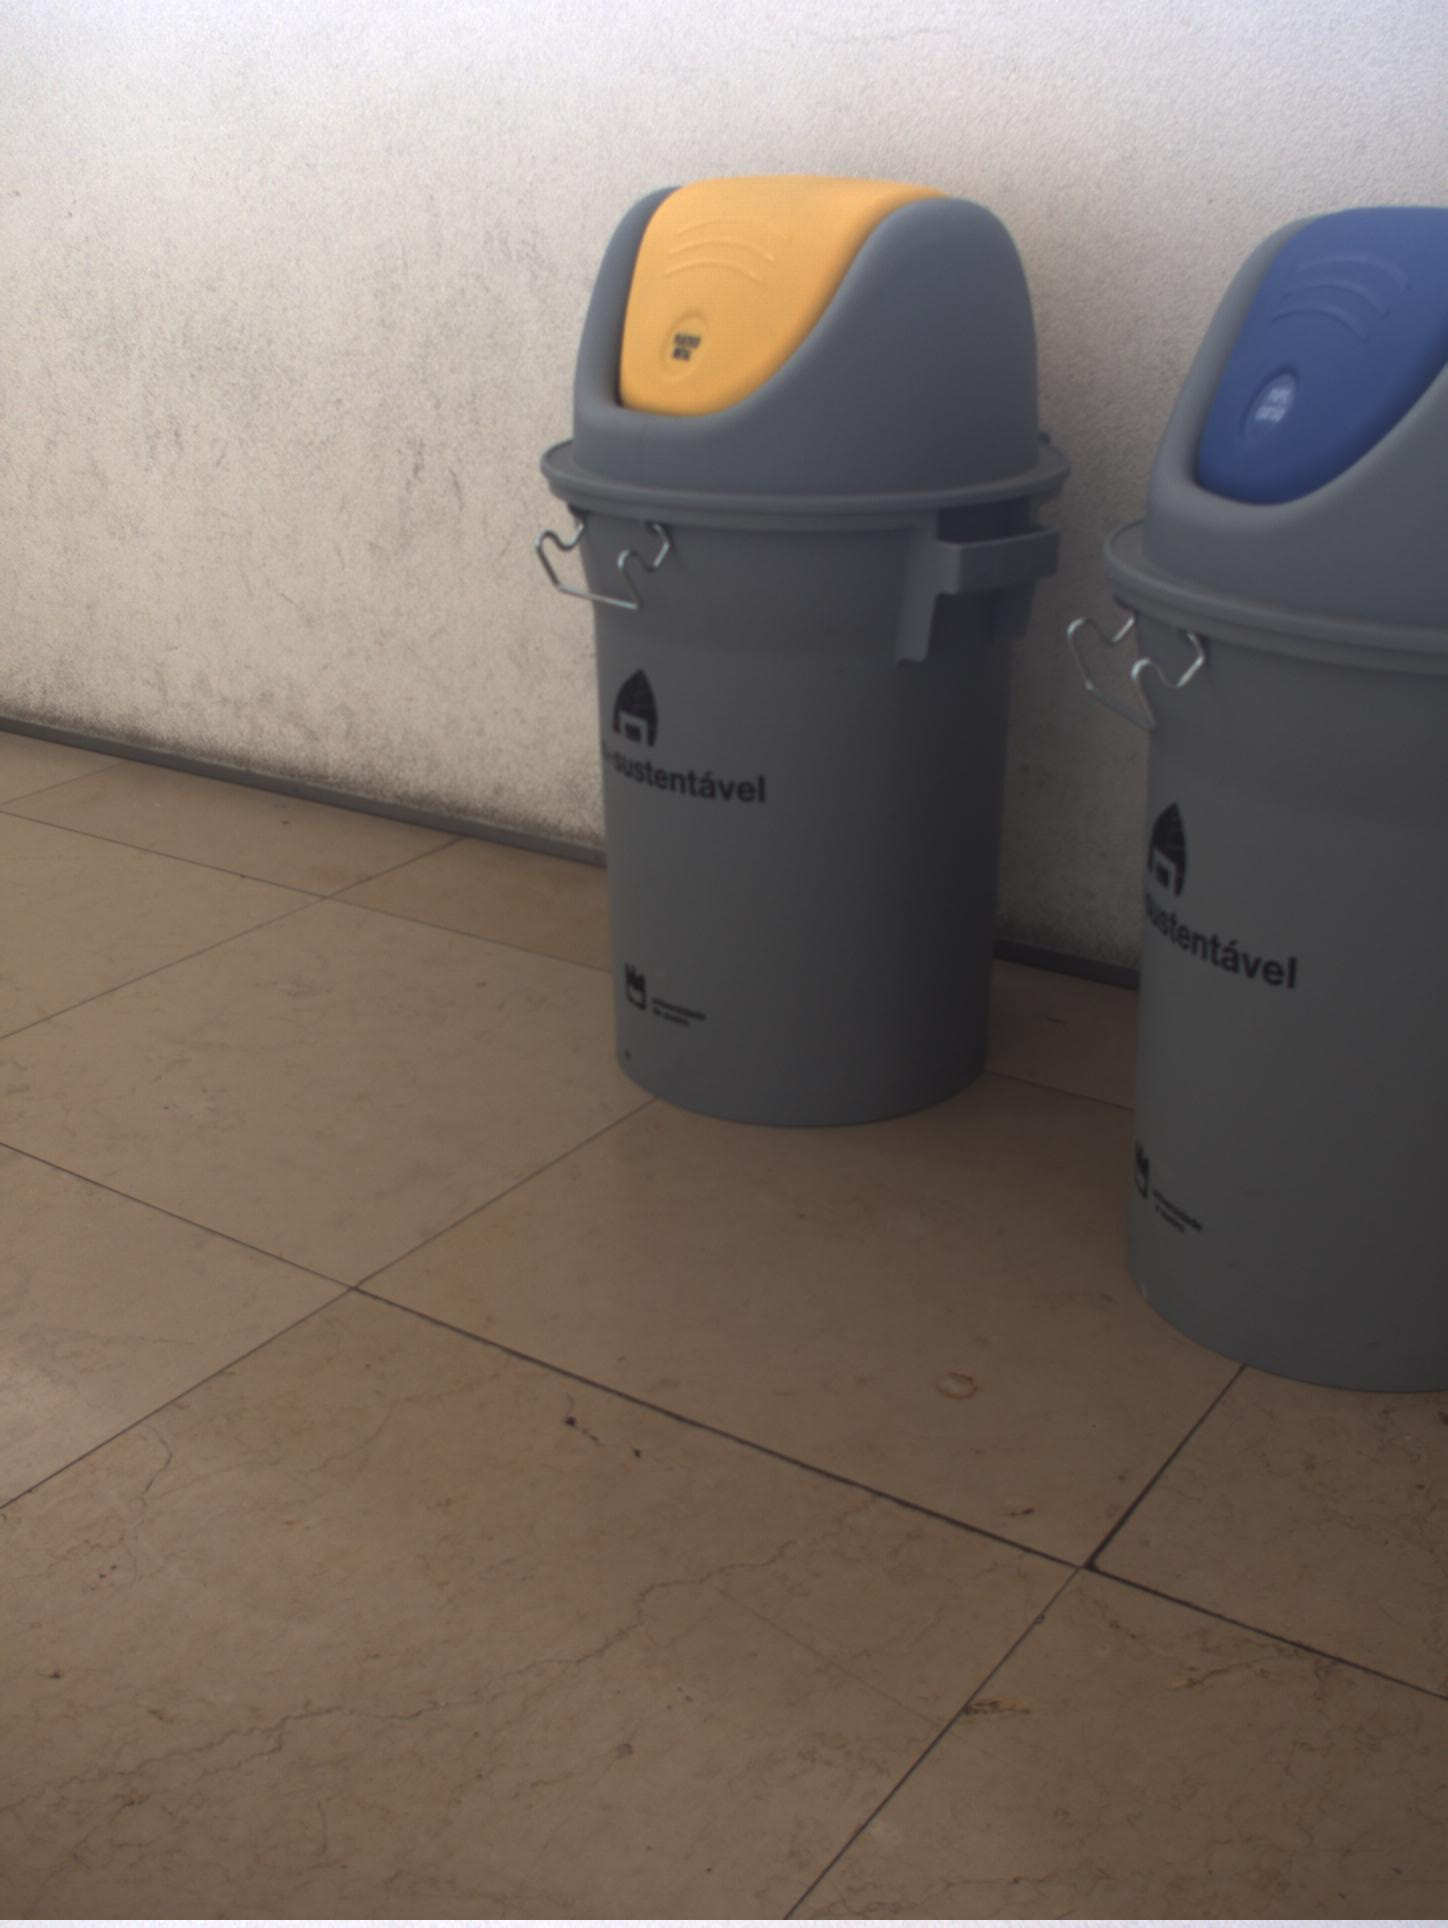
\includegraphics[width=0.6\textwidth]{illumination-issues-0}
    \end{subfigure}%
    \begin{subfigure}{0.5\textwidth}
        \centering
        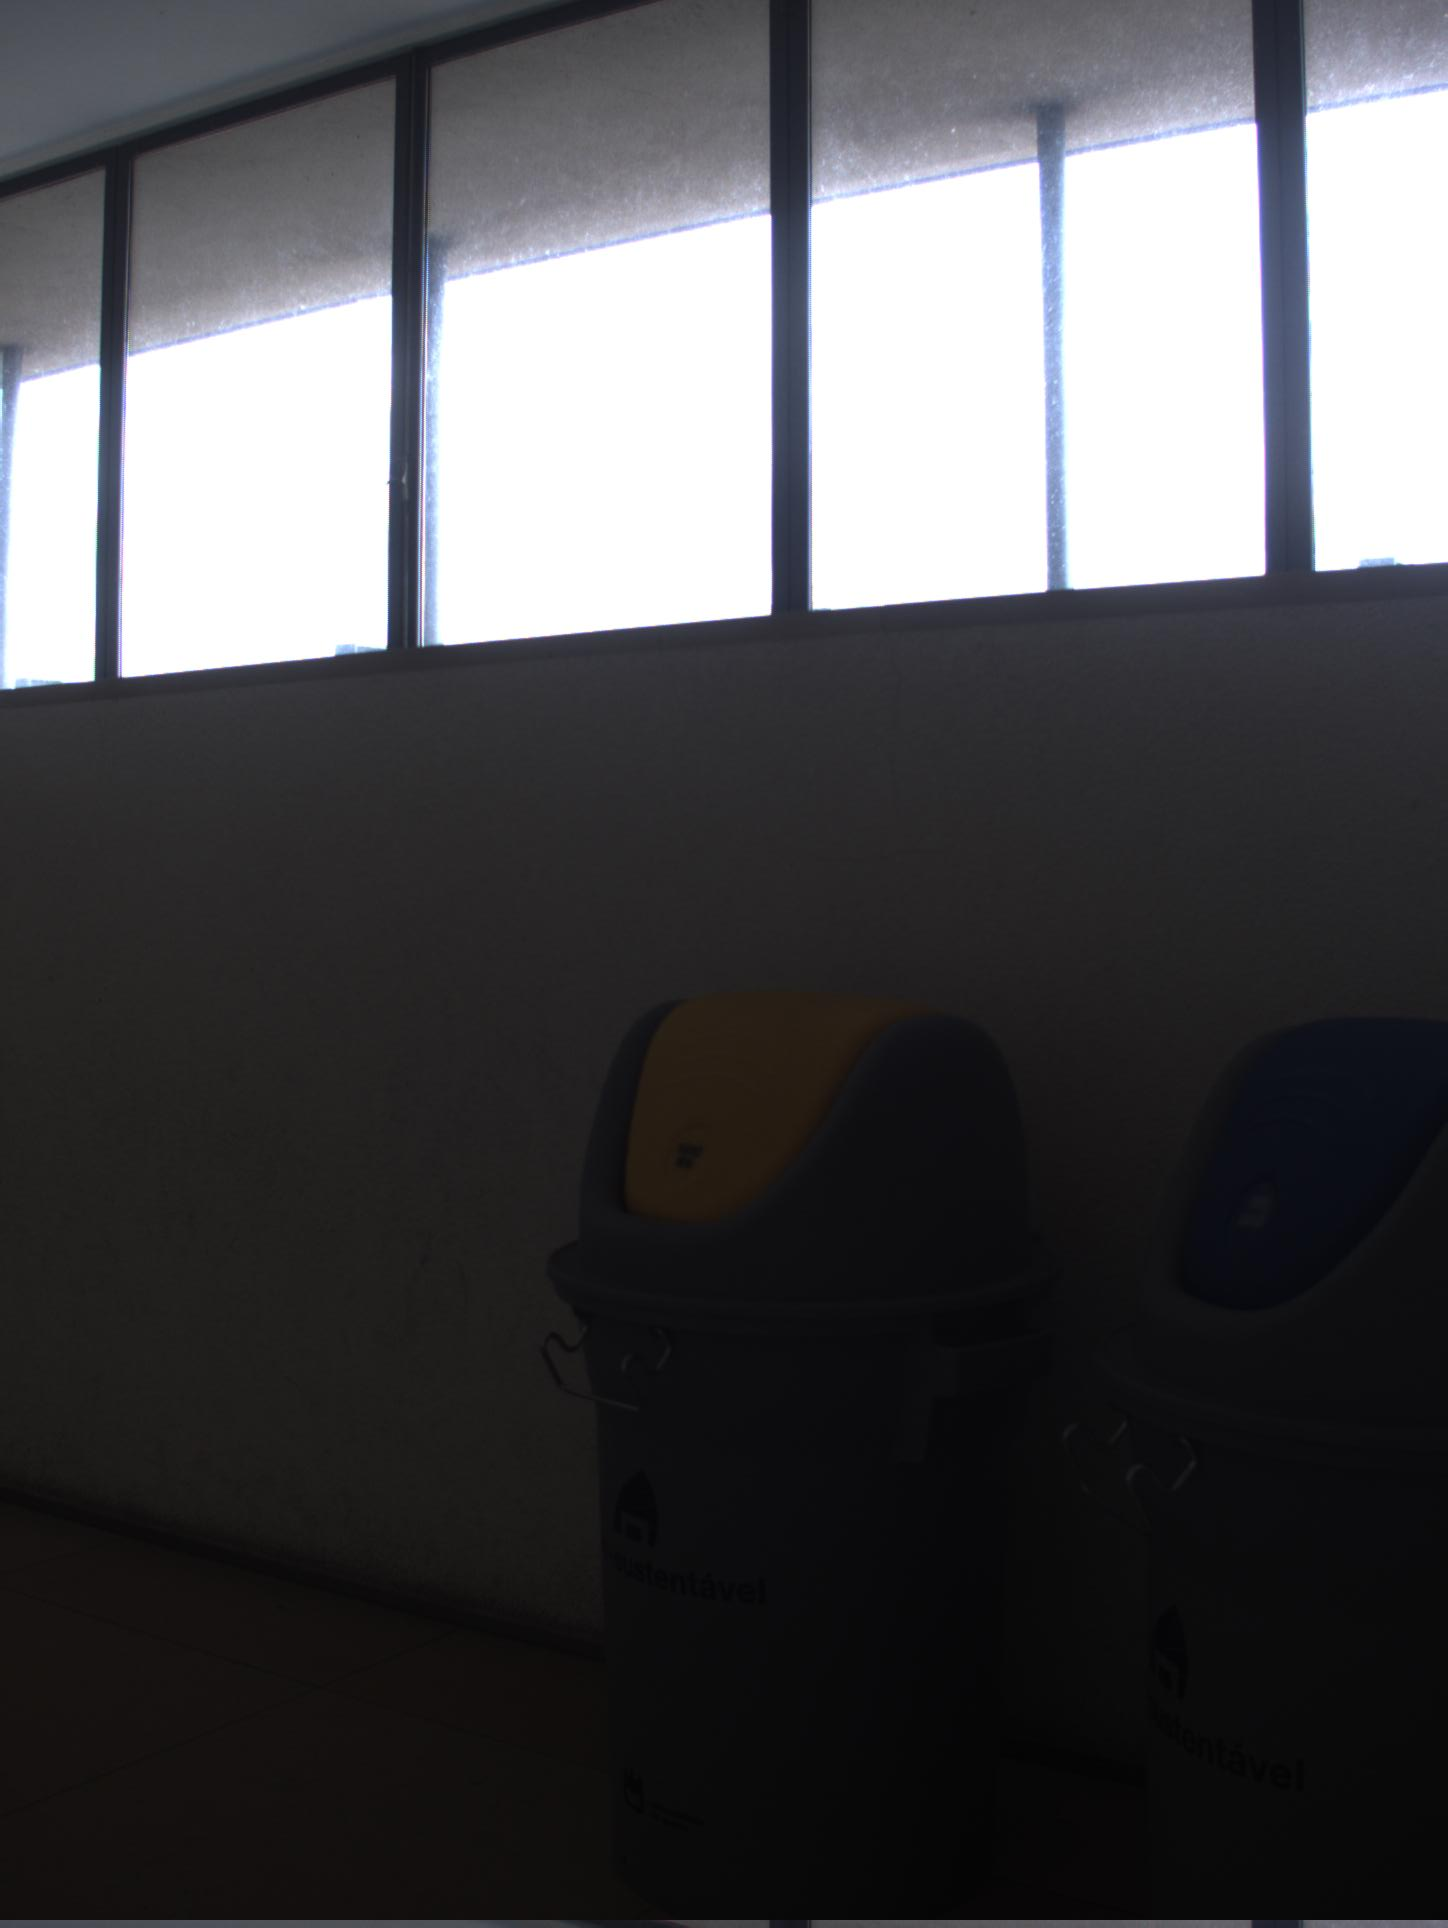
\includegraphics[width=0.6\textwidth]{illumination-issues-1}
    \end{subfigure}%

    \caption{Two images taken on the same acquisition with different colors.}
    \label{figure:illumination-issues-images}

\end{figure}

\begin{figure}[h]
    
    \centering
    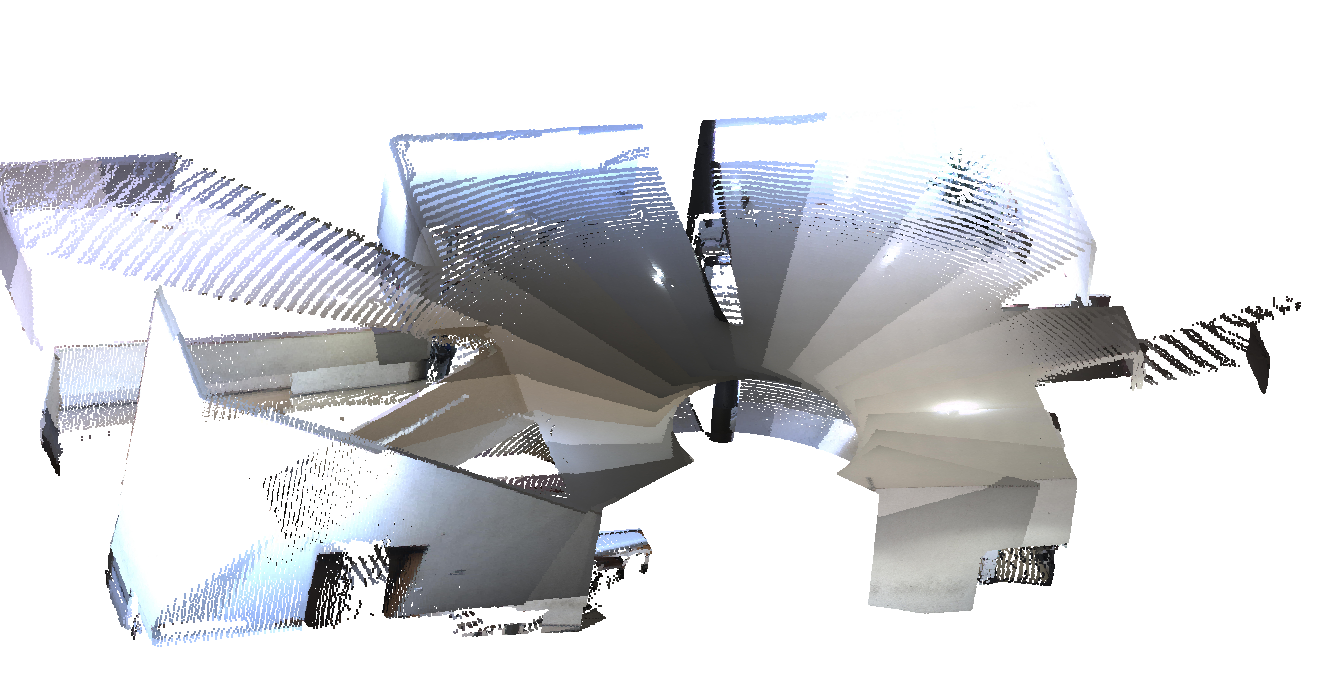
\includegraphics[width=0.8\textwidth]{color-registration-mean-4}

    \caption{Illumination issues in the point cloud.}
    \label{figure:illumination-issues-pointcloud}

\end{figure}

The color fusion techniques also have a great effect on the final result. The colors look sharper if the chosen method is the first, last or the closest method, but discontinuities caused by the imperfect registration are more noticeable. On the other hand, mean methods results in a blurring effect on the colors, but the discontinuities are less noticeable. In general, the mean fusion produces the best result overall, but the small details are smudged. The closest color fusion produces the sharpest result, so the small details are visible, however, it yields the worst quality overall. The two results can be seen in \cref{figure:fusion-methods-closest,figure:fusion-methods-mean}.

\begin{figure}[h]
    
    \centering
    \begin{subfigure}[t]{0.7\textwidth}
        \centering
        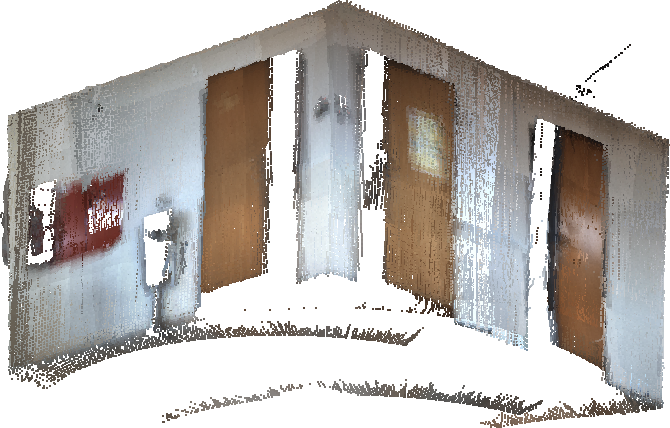
\includegraphics[width=0.9\textwidth]{color-registration-2}

        \caption{Mean color fusion method.}
        \label{figure:fusion-methods-mean}
    \end{subfigure}

    \begin{subfigure}[t]{0.7\textwidth}
        \centering
        \includegraphics[width=0.9\textwidth]{color-registration-5}

        \caption{Closest color fusion method.}
        \label{figure:fusion-methods-closest}
    \end{subfigure}%

    \caption{Comparison of two color fusion methods.}
    \label{figure:fusion-methods-1}

\end{figure}

Moreover, the mean method still shows some discontinuities and edges. To improve the blending of the colors, this work proposes a weighted mean, based on two factors: $f_1$ and $f_2$. This factors prioritize colors that are taken closer to the point or taken closer to the center point of the camera. In \cref{figure:fusion-methods-f1,figure:fusion-methods-f2}, this two color fusion methods are compared against the closest color method, present in \cref{figure:fusion-methods-mean}. As seen, both methods have overall better results, specially in the blending of the different colors, and reducing the transitions between images.

\begin{figure}[h]
    
    \centering
    \begin{subfigure}[t]{\textwidth}
        \centering
        \includegraphics[width=0.6\textwidth]{color-registration-comparizon-last}

        \caption{Last color fusion method.}
        \label{figure:fusion-methods-mean}
    \end{subfigure}

    \begin{subfigure}[t]{\textwidth}
        \centering
        \includegraphics[width=0.6\textwidth]{color-registration-comparizon-f1}

        \caption{Weighted mean with factor $f_1$ color fusion method.}
        \label{figure:fusion-methods-f1}
    \end{subfigure}%

    \begin{subfigure}[t]{\textwidth}
        \centering
        \includegraphics[width=0.6\textwidth]{color-registration-comparizon-f2}

        \caption{Weighted mean with factor $f_2$ color fusion method.}
        \label{figure:fusion-methods-f2}
    \end{subfigure}

    \caption{Comparison of two weighted mean color fusion methods.}
    \label{figure:fusion-methods-2}

\end{figure}

Finally, the color reconstruction method successfully colorized the point clouds, as seen in \cref{figure:full-color-registration}. However, the results are far from perfect, due to the inconsistent color in different images and the sub-optimal calibration of the camera.

\begin{figure}[h]
    
    \centering
    \includegraphics[width=\textwidth]{color-registration-last-3}

    \caption{Full color registration of one point cloud.}
    \label{figure:full-color-registration}
\end{figure}
\chapter{Conclusions and Future Work}
\label{section:conclusions-and-future-work}

\label{Conclusions}
\label{section:conclusions}

3D reconstruction of real world scenes has been and still is an important field today with many applications. The most promising technology relies on LiDAR laser scanners and cameras to capture both the geometry and color information of the scene. However, the fusion of the data of both sensors still has some issues. This work presents a methodology for both the capture process, as well as the algorithms to reconstruct the geometry and the color information from the laser scanner and camera data. 

First, a 3D scanner was developed, in order to obtain the data required. This 3D scanner is composed, at its core, by a pan and tilt unit, a 3D laser scanner and a camera. In particular, three laser scanners were used, to test the validity of the reconstruction algorithms and also to study the influence of the laser scanner in the final result.

The scene capturing methodology describes a method to minimize the technical limitations of the sensors, so that the scene capture is not influenced by them. Hence, each capture is composed by several acquisitions, that are taken from different poses in the scene. In each acquisition, the PTU joints moves though multiple waypoints and multiple images and laser scans are recorded during this movement. The pose and number of acquisitions should be adequate such that every part of the scene is recorded. However, this planning is done a priori, so it is not always certain that the scene is totally captured, as seen in the results.

The first reconstruction is the geometric reconstruction, which uses the laser scanner data and the PTU transformations to reconstruct the geometry, resulting in a point cloud. This reconstruction relies on an accurate calibration of the laser scanner to the PTU frame, which is called the extrinsic laser calibration. The first attempt of this calibration was with the RADLOCC calibration. This was, however, unsuccessful, because the calibrations yield by it still produced point clouds with visible deformation. Therefore, a new method was developed which has superior results and the point cloud produced by it does not have noticeable deformations. Furthermore, a normal estimation method was developed that exploits the bi-dimensional structure of the point cloud obtained to estimate the normals. This method is faster than the more standard method using the $k$-neighbors without sacrificing the overall result. However, this method is sensible to inconsistencies in the movement of the PTU, specially at the interruptions using to capture the images. Finally, the registration of multiple acquisitions was done using the ICP method. However, this method was sub-optimal, because the registration failed if the initial estimate of the transformations were not close to the correct transformation. To bypass this problem, the initial estimate was done manually first. Also, the ICP method is limited to a pairwise registration, so three methods were tried to apply the ICP to multiple point clouds. Overall, the geometric registration was successful and the resulting point cloud is dense and accurate. 

The next stage in the reconstruction was the color reconstruction, which uses the image taken from the camera to attribute colors to the point cloud previously obtained. This reconstruction was separated into two steps. First, each image is registered in the point cloud, by re-projection of the points in the image surface. Then, the points that are outside the visual frustum of the camera and the points that are occluded are removed. Finally, the color correspondent to each projected point is obtained using a bilinear interpolation. After this step, each image has a correspondent partial colorization of the point cloud. This step relies on the projection matrix and extrinsic transformation of the camera to register the points in the image, which are obtained via the intrinsic calibration and extrinsic camera calibration. Then, each point has multiple colors associated, but an unique color has to be chosen for each point, which is done in the color fusion step. Multiple fusion techniques were tried, as choosing the first, last or closest color from all the registered colors, or by calculating the average color of the registered colors. Overall, the color reconstruction is not optimal due to several factors. First, the images vary in hue or intensity, due to factors during the capture, like the lightning of the scene. This creates inconsistencies in the colorization point cloud that are really noticeable in the final results. Secondly, the extrinsic of the camera is not accurate, so the color registration is imperfect. 

Overall, the results are satisfactory, specially the geometric registration. There are, however, numerous limitation on both registrations that require to be solved, for example, a better extrinsic camera calibration, or an automatic acquisition registration method.

\subsection{Future Work}
\label{section:future-work}

The methodologies explored in this work still leave much room for exploration and development. Some algorithms and methods have shortcomings in their performance and usability. Hereby, some possible solutions and thoughts that could be explored and developed in the future work are described. In particular, possible solutions for the acquisition registration, color normalization and camera extrinsic calibration are discussed.

The acquisition registration can be improved in two approaches. The first approach could be the integration of some localization device in the robot, as for example a inertial measurement unit, which can be used to obtain an approximate transformation between the acquisitions. This approximate solution could replace the initial estimate done manually in this work. The second approach world be to improve or modify the ICP algorithm, because of its disadvantages. Firstly, the new algorithm should be able to register multiple point clouds at once, instead of just two. This algorithm world probably have a better accuracy than the methods used in this work. Also, the distance between point clouds, which is the heuristic of the ICP algorithms should be modified, because most times it is incorrect and is only successfully if the two point clouds are very close. Instead, features could be extracted from the point clouds, for example, edges and corners, and their distance should be used instead. Because this features are sparse, it is possible that this correspondence is more accurate.

Moreover, the images obtained should have a similar color for the same object, which is not the case, due to the different illumination. So, a normalization of the images should be done prior to any color registration phase. Also, the use of high dynamic range photography should be used to improve this normalization. As a result, the colors of the same objects should be the same across all the images, and this color should be independent of the lightning of the scene.

Furthermore, a new calibration method to obtain the extrinsic calibration of the camera should be developed. The principal limitations of the hand-in-eye algorithms, is the fact that only a small portion of the angle interval of the joint angles are used for the calibration, and the ArUCO pose estimation has an high error. Recently, in the master thesis of Filipe Costa \cite{costa18}, a bundle calibration method of ArUCO markers and camera was developed. With small adjustments, this algorithm can be modified to calibrate a camera mounted on a PTU. More specifically, this calibration obtains a precise pose of the camera and all the ArUCO markers, which could be considered to fed the original hand-in-eye algorithms, with the change that now there are multiple markers instead of just one. It is possible that this method could achieve better results that the original hand-in-eye method used in this work.

Finally, some abnormalities were found in the laser scans produced by the 2D laser scanner SICK LMS100, which undermined its use. The source of the problem was not identified in this work, but it should be found. 

\printbibliography

\end{document}